\documentclass[11pt]{article}
\usepackage{amsmath,amsfonts, bbm,amssymb, amsthm, tikz-cd}
\usepackage{stmaryrd} %para \ogreaterthan
\usepackage{geometry}
\usepackage{enumitem}
\usepackage[colorlinks=true, linkcolor=blue]{hyperref}
\usepackage{mathrsfs}
\usepackage{tocloft}
\usepackage[capitalize]{cleveref} 

\geometry{margin=1in}

\renewcommand{\cftsecleader}{\cftdotfill{\cftdotsep}}
\setlength{\cftbeforesecskip}{5pt}



\newcommand{\cat}[1]{\mathcal{#1}}
\newcommand{\field}{\Bbbk}
\newcommand{\N}{\mathbb{N}}
\newcommand{\Hom}{\mathrm{Hom}}
\newcommand{\End}{\mathrm{End}}
\newcommand{\Tr}{\mathrm{Tr}}
\newcommand{\C}{\mathcal{C}}
\newcommand{\Rexf}{\mathsf{Rex}^{\mathsf{f}}}
\newcommand{\Surf}{\mathsf{Surf}}
\newcommand{\OSurf}{\mathsf{OSurf}}
\newcommand{\Hbdy}{\mathsf{Hdby}}
\newcommand{\Alg}{\mathsf{Alg}}
\newcommand{\CycAlg}{\mathsf{CycAlg}}
\newcommand{\ModAlg}{\mathsf{ModAlg}}
\newcommand{\As}{\mathsf{As}}
\newcommand{\cA}{\mathcal{A}}






\newtheorem{theorem}{Theorem}[section]
\newtheorem{proposition}[theorem]{Proposition}
\newtheorem{lemma}[theorem]{Lemma}
\newtheorem{corollary}[theorem]{Corollary}
\newtheorem{conjecture}[theorem]{Conjecture}
\newtheorem{problem}[theorem]{Problem}
\newtheorem{question}[theorem]{Question}


\theoremstyle{definition}
\newtheorem{definition}[theorem]{Definition}
\newtheorem{example}[theorem]{Example}
\newtheorem{examples}[theorem]{Examples}
\newtheorem{construction}[theorem]{Construction}





\title{The Category Zoo \\{\small Rough, unfinished notes! Use at your own risk.}}
%\date{}
\author{Jorge Becerra}
\begin{document}
\maketitle

\tableofcontents

\vspace{1cm}

These notes have been partially written copying snippets from the ChatGPT/Gemini AIs. Use at your own risk!

The author would like to thank Lukas Woike for explaining and clarifying to him many of the ideas appearing here.



\section{Linear Categories}

\subsection{Semiadditive category}
A category with a zero object (i.e., both initial and terminal object; and therefore zero morphisms) and with
finite products and coproducts in which the canonical map
\[
\coprod_i X_i \to \prod_i X_i
\]
is an isomorphism---hence finite biproducts exist, and these are typically called direct sums $\oplus$.

\subsection{Additive category}
Any preadditive category is naturally enriched over commutative monoids: given maps $f, g: X \to Y$, define
$f+g$ as the composite:
\[
X \to X \times X \cong X \amalg X \to Y \times Y \cong Y \amalg Y \to Y
\]
where the first map is the diagonal map $(\mathrm{id}, \mathrm{id})$, the second map is $(f,0) \amalg (0,g)$, and the third
one is $\mathrm{id} \amalg \mathrm{id}$.

If such an enrichment extends to abelian groups, that is, if every map $f$ has an inverse $-f$ for the
previously defined sum, then the category is said to be an additive category.

Alternatively, additive means $\mathsf{Ab}$-enriched plus finite products and coproducts exist (and because of the
enrichment they are automatically isomorphic). Typically, the biproduct is represented by the direct sum sign $\oplus$.

A functor between additive categories is additive if it preserves the finite biproducts, i.e., $F(0) = 0$ and $F(X \oplus Y) \cong F(X) \oplus F(Y)$.

\subsection{Preadditive category}
A category enriched over abelian groups.

\subsection{$\Bbbk$-linear category or $\Bbbk$-category}
A category enriched over $\Bbbk$-modules, where $\Bbbk$ is a commutative ring with unit. A linear category might \emph{not} be additive (finite biproducts might not exist).

A functor between $\Bbbk$-linear categories is linear if $F_{X,Y}$ between the hom's is a linear map. Linear functors are automatically additive, i.e., they preserve the biproducts.

\subsection{Additive envelope}
As mentioned before, a linear category might not have all finite biproducts. But it always embeds into a category that has them. The additive envelope $\mathsf{Add}(\mathcal{C})$ of a linear category $\mathcal{C}$ has objects formal direct sums $\bigoplus_i X_i$ of objects of $\mathcal{C}$ and arrows given by matrices of arrows in $\mathcal{C}$, with composition modelled by matrix
multiplication. There is a canonical functor $\mathcal{C} \hookrightarrow \mathsf{Add}(\mathcal{C})$, and it is determined by the universal property that if $\mathcal{D}$ has all finite biproducts, then there is a bijection
\[
\mathrm{LinFun}(\mathcal{C}, \mathcal{D}) \cong \mathrm{LinFun}(\mathsf{Add}(\mathcal{C}), \mathcal{D})
\]

\subsection{Karoubi envelope}
Remember that an idempotent in a category is an endomorphism $f: X \to X$ of a certain object such that $f \circ f = f$. A splitting for an idempotent $f$ is a pair of arrows $r: Y \to X$ and $s: Y \to X$ such that $s \circ r = f$ and $r \circ s = \mathrm{id}_Y$. Splittings for idempotents are unique up to unique isomorphism.

A category $\mathcal{C}$ is idempotent complete or Karoubian if all idempotents split. A linear category might have idempotents that do not split. But it always embeds into a category where they do. The Karoubian envelope or idempotent completion $\mathsf{Kar}(\mathcal{C})$ of a linear category $\mathcal{C}$ has objects idempotents $f: X \to X$ (more precisely pairs $(X,f)$).

An arrow between two idempotents $(X,f)$ and $(Y,g)$ is an arrow $h: X \to Y$ such that $h = g \circ h \circ f$, with composition taken from $\mathcal{C}$. There is a canonical functor $\mathcal{C} \hookrightarrow \mathsf{Kar}(\mathcal{C})$, taking $X$ to $(X, \mathrm{id})$, and it is determined by the universal property that if $\mathcal{D}$ is idempotent complete, then there is a bijection
\[
\mathrm{LinFun}(\mathcal{C}, \mathcal{D}) \cong \mathrm{LinFun}(\mathsf{Kar}(\mathcal{C}), \mathcal{D})
\]

\subsection{Cauchy completion}
A linear category is Cauchy complete if it has all finite biproducts and it is idempotent complete. The Cauchy completion of $\mathcal{C}$ is $\mathsf{Cauchy}(\mathcal{C}) := \mathsf{Kar}(\mathsf{Add}(\mathcal{C}))$ (warning: this is \emph{not} equivalent to $\mathsf{Add}(\mathsf{Kar}(\mathcal{C}))$).

Every linear abelian category is Cauchy complete; the converse is not true.

\subsection{Simple objects (non-abelian version)}
If $X$ is an object of a $\Bbbk$-linear category, then $\mathrm{End}(X)$ is naturally a $\Bbbk$-algebra with
unit the identity. It is not hard to see that the following items are equivalent:
\begin{enumerate}[label=(\roman*)]
    \item the map $\Bbbk \to \operatorname{End}_{\mathcal{C}}(X),\; k \mapsto k \cdot \mathrm{id}$ is an isomorphism of $\Bbbk$-modules;
    \item the map $\Bbbk \to \operatorname{End}_{\mathcal{C}}(X),\; k \mapsto k \cdot \mathrm{id}$ is an isomorphism of $\Bbbk$-algebras;
    \item the $\Bbbk$-algebra $\operatorname{End}_{\mathcal{C}}(X)$ is isomorphic to $\Bbbk$;
    \item the $\Bbbk$-module $\operatorname{End}_{\mathcal{C}}(X)$ is free of rank 1.
\end{enumerate}
If an object $X$ satisfies any of these equivalent descriptions, we say that $X$ is simple.

\subsection{Semisimple category (non-abelian version)}
Suppose $\mathcal{C}$ is a Cauchy complete linear category whose isomorphism classes of objects form a set. Then the following conditions are equivalent:
\begin{itemize}
    \item[(S)] There is a set $S$ and an equivalence of categories $\mathcal{C} \cong \mathrm{Vec}_{\mathrm{fd}}(S)$ (the category of $S$-graded vector spaces and grading-preserving maps).
    \item[(End)] For every object $X \in \mathcal{C}$, the endomorphism space $\mathrm{End}(X)$ is a finite-dimensional complex semisimple algebra, i.e., a multimatrix algebra.
    \item[(Obj)] Every $X \in \mathcal{C}$ is isomorphic to a finite direct sum of simple objects $X = \bigoplus_{i=1}^n X_i$, where each pair $X_i, X_j$ are either isomorphic or distinct.
    \item[(M\"uger)] There is a set of pairwise distinct simple objects $\{X_s\}_{s \in S}$ such that for any $A,B \in \mathcal{C}$, the composition map
    \[
    \bigoplus_{s \in S} \mathcal{C}(A \to X_s) \otimes_{\Bbbk} \mathcal{C}(X_s \to B) \xrightarrow{\circ} \mathcal{C}(A \to B)
    \]
    is an isomorphism. (The direct sum is taken in the category of finite-dimensional vector spaces.)
\end{itemize}

Being \emph{finitely} semisimple means that $S$ is a finite set, i.e., there are finitely many isomorphism classes of simple objects.

\medskip

\noindent\textbf{Fact:} A Cauchy complete linear category is semisimple if and only if it is abelian and all short exact sequences split.

\medskip

\noindent\textbf{More important fact:} Linearity and object semisimplicity already imply abelianness! See Section \ref{lnear_and_ss_imply_abelian}.


\subsection{Generators}


Let $\C$ be an additive category. An object $G \in \C$ is called a generator if any object of $\C$ is a quotient of some direct sum of copies of $G$, that is, if there is an epimorphism $G^{\oplus n} \twoheadrightarrow X$.\medskip


\noindent \textbf{Lemma.} $G$ is a generator if and only if $Hom(G,-)$ is faithful.

\begin{proof}
Let $\mathcal C$ be an additive category and $G \in \mathcal C$.

\textbf{Step 1: If $G$ is a generator, then $\mathrm{Hom}(G,-)$ is faithful.}

Suppose $G$ is a generator. By definition, for every $X \in \mathcal C$, there exists an epimorphism
\[
f: G^{\oplus I} \twoheadrightarrow X
\]
for some index set $I$.

Let $g: X \to Y$ be a morphism such that $\mathrm{Hom}(G,g) = 0$. We want to show $g=0$.

Consider the composition $g \circ f: G^{\oplus I} \to Y$. Since $\mathrm{Hom}(G,g)=0$, it follows that $g \circ f = 0$. But $f$ is an epimorphism, so $g=0$. Therefore, $\mathrm{Hom}(G,-)$ is faithful.

\textbf{Step 2: If $\mathrm{Hom}(G,-)$ is faithful, then $G$ is a generator.}

Suppose $\mathrm{Hom}(G,-)$ is faithful. Let $X \in \mathcal C$ be arbitrary. Consider the morphism
\[
c: \bigoplus_{f \in \mathrm{Hom}(G,X)} G \longrightarrow X
\]
which sends the $f$-th copy of $G$ via $f$ to $X$. We claim that $c$ is an epimorphism.

Indeed, suppose $h: X \to Y$ satisfies $h \circ c = 0$. Then for every $f \in \mathrm{Hom}(G,X)$, we have $h \circ f = 0$. By the faithfulness of $\mathrm{Hom}(G,-)$, this implies $h=0$. Hence $c$ is an epimorphism, and $X$ is a quotient of a sum of copies of $G$.
\end{proof}
 


\section{Miscellaneous}

\subsection{Action groupoid}

If $G$ is a group and $X$ is a $G$-set, the \textit{action groupoid} $X /\!\!/ G$ is the groupoid (=cat with all arrows isos) with objects the elements and $X$, and an arrow $x \to y$ is a $g \in G$ such that $gx=y$. Composition = multiplication on $G$.

This specialises to the usual way of viewing a group $G$ as a groupoid with one object and arrows $G$. This is then $* /\!\!/ G$.




\subsection{Action of a group on  a category}


Recall that if $X$ is a set or a topological space, a $G$-set or a $G$-space is the same as a functor $X: * /\!\!/ G  \to \mathsf{Set} \ / \ \mathsf{Top}$.

Now let us view $* /\!\!/ G$ as a 2-category with only identity 2-cells, and let $\mathsf{Cat}$ be the 2-category of categories, functors and natural transformations. Then a (non-strict/homotopy) action of $G$ on a category $\C$ is a pseudofunctor $\C : * /\!\!/ G \to \mathsf{Cat}$.


Explicitly, this is the data of: for every $g \in G$, an equivalence $\varphi_g: \C \overset{\simeq}{\to} \C$ , together with the data of natural isos $\varphi_g \varphi_h \cong \varphi_{gh}$, subject to the associativity condition that the isomorphism $\varphi_g \varphi_h \varphi_k \cong \varphi_g \varphi_{hk} \cong \varphi_{ghk}$ equals the iso $\varphi_g \varphi_h \varphi_k \cong \varphi_{gh} \varphi_{k} \cong \varphi_{ghk}$.


Alternative point of view: regard $G$ as a discrete strict monoidal category with monoidal product equals the product of $G$. Recall that $\mathsf{End}(\C)$ is a monoidal category with monoidal product composition. Then an action of $G$ on $\C$ amounts to the data of a strong monoidal functor $G \to \mathsf{End}(\C)$.

For an object $X \in \C$ we write $g.X := \varphi_g(X)$.

\subsection{Homotopy fixed point for an action on a category}


Let $\C$ be a $G$-category. A \textit{homotopy fixed point} is the data of an object $X \in \C$ together with isomorphisms $\alpha_g : g.X \overset{\cong}{\to} X$ satisfying
$$
\begin{tikzcd}
    h.g.X \rar{h \alpha_g} \dar{\cong} & h.X \rar{\alpha_h} & X\\
    (hg).X \arrow{urr}[swap]{\alpha_{hg}}
\end{tikzcd}
$$


The category $\C^{hG}$ of homotopy fixed points has objects htpy fixed points and  arrows maps $f:X \to Y$ in $\C$ such that
$$
\begin{tikzcd}
    g.X \rar{\alpha_g} \dar{g.f} & X \dar{f} \\
    g.Y \rar{\alpha'_g} & Y
\end{tikzcd}
$$

\section{Limits and Colimits}

\subsection{Kernel (via equalizer/pullback)}
Let $\mathcal{C}$ be a category with a zero object $0$ (an object that is both initial and terminal) and suppose equalizers exist in $\mathcal{C}$. For a morphism $f: X \to Y$, the zero morphism $0_{XY}: X \to Y$ is the unique factorization of $X \to 0 \to Y$.

The \textbf{kernel} of $f$ can be defined as the equalizer of the pair of parallel morphisms $f$ and $0_{XY}$:
\[
\ker(f) \xrightarrow{k} X \rightrightarrows^{f}_{0_{XY}} Y.
\]
That is, $k: \ker(f) \to X$ is an object and morphism such that $f \circ k = 0_{XY} \circ k (= 0_{\ker(f), Y})$ and it is universal with this property (any other $g: Z \to X$ with $f \circ g = 0_{XY} \circ g$ factors uniquely through $k$).

Since $0$ is initial, the morphism $0 \to X$ exists uniquely. Since $0$ is terminal, the morphism $X \to 0$ exists uniquely. Their composite $X \to 0 \to Y$ is the zero morphism $0_{XY}$.

Alternatively, in a category $\mathcal{C}$ with a zero object $0$ (which is both initial and terminal) and pullbacks, the \textbf{kernel} of a morphism $f: X \to Y$ can be defined using a pullback.

Specifically, the kernel $k: \ker(f) \to X$ is the pullback of $f$ along the unique zero morphism $0_Y: 0 \to Y$. The pullback diagram is:
\[
\begin{tikzcd}
\ker(f) \arrow[r] \arrow[d, "k"'] & 0 \arrow[d, "0_Y"] \\
X \arrow[r, "f"'] & Y
\end{tikzcd}
\]

The map $k$ automatically satisfies $f \circ k = 0$, and the universal property of the pullback ensures that $k$ is universal among all maps into $X$ whose composition with $f$ is zero.



\subsection{Cokernel (via Coequalizer)}
Dually, let $\mathcal{C}$ be a category with a zero object $0$ and suppose coequalizers exist. For a morphism $f: X \to Y$, consider the zero morphism $0_{XY}: X \to Y$.

The \textbf{cokernel} of $f$ can be defined as the coequalizer of the pair $f$ and $0_{XY}$:
\[
X \rightrightarrows^{f}_{0_{XY}} Y \xrightarrow{q} \operatorname{coker}(f).
\]
That is, $q: Y \to \operatorname{coker}(f)$ is an object and morphism such that $q \circ f = q \circ 0_{XY} (= 0_{X, \operatorname{coker}(f)})$ and it is universal with this property (any other $g: Y \to Z$ with $g \circ f = g \circ 0_{XY}$ factors uniquely through $q$).

\subsection{Left/Right Exact Functors}
Let $F: \mathcal{C} \to \mathcal{D}$ be a functor between categories where certain limits or colimits exist.

The functor $F$ is \textbf{left exact} if it preserves all finite limits that exist in $\mathcal{C}$. This means that if $L$ is the limit of a finite diagram $D: J \to \mathcal{C}$ (where $J$ is a finite category), then $F(L)$ is the limit of the diagram $F \circ D: J \to \mathcal{D}$. Common examples include preserving terminal objects, products, and equalizers (and thus pullbacks and kernels if they exist).

The functor $F$ is \textbf{right exact} if it preserves all finite colimits that exist in $\mathcal{C}$. This means that if $C$ is the colimit of a finite diagram $D: J \to \mathcal{C}$, then $F(C)$ is the colimit of the diagram $F \circ D: J \to \mathcal{D}$. Common examples include preserving initial objects, coproducts, and coequalizers (and thus pushouts and cokernels if they exist).

A functor is \textbf{exact} if it is both left exact and right exact (preserves all finite limits and finite colimits).

In the context of abelian categories, these definitions are equivalent to the definitions involving preservation of kernels/cokernels or exact sequences, assuming the functor is also additive.


\subsection{RAPL / LAPC}

Right Adjoints Preserve Limits, in particular right adjoints are left exact.

Left Adjoints Preserve Colimits, in particular left adjoints are right exact.

For finite abelian categories (see later), it is actually an iff.


Perhaps a better way to remember this: 

\begin{center}
\textbf{L}eft adjoints preserve\textbf{ L}imits IS WRONG.
\end{center} 


\subsection{Linear functor + source semisimple imply exact}


If $F: \mathcal{C} \to \cat{D}$ is a linear (additive) functor between linear abelian categories and $\cat{C}$ is semisimple, then $F$ is exact.

This follows as in $\cat{C}$ short exact sequences split and then by additivity so do the images under $F$.


In particular any linear functor $\mathsf{vect} \to \cat{A}$ is exact.

\subsection{Pullbacks from Products and Equalizers}
The existence of pullbacks in a category $\mathcal{C}$ is closely related to the existence of binary products and equalizers.

Specifically, if a category $\mathcal{C}$ has all binary products and all equalizers, then it has all pullbacks. To construct the pullback of a diagram $X \xrightarrow{f} Z \xleftarrow{g} Y$:
\begin{enumerate}
    \item Form the binary product $X \times Y$ with its projection morphisms $p_X: X \times Y \to X$ and $p_Y: X \times Y \to Y$.
    \item Consider the two morphisms from the product to $Z$: $f \circ p_X : X \times Y \to Z$ and $g \circ p_Y : X \times Y \to Z$.
    \item Take the equalizer $e: P \to X \times Y$ of this pair:
    \[
    P \xrightarrow{e} X \times Y \rightrightarrows^{f \circ p_X}_{g \circ p_Y} Z.
    \]
\end{enumerate}
The resulting object $P$ together with the morphisms $p_1 = p_X \circ e : P \to X$ and $p_2 = p_Y \circ e : P \to Y$ forms the pullback square:
\[
\begin{tikzcd}
P \arrow[r, "p_2"] \arrow[d, "p_1"'] & Y \arrow[d, "g"] \\
X \arrow[r, "f"'] & Z
\end{tikzcd}
\]

Conversely, if a category has all pullbacks and a terminal object (which acts as the empty product), it has all finite products. If it has pullbacks and products, it also has equalizers (an equalizer of $h, k: A \to B$ is the pullback of $(h, k): A \to B \times B$ along the diagonal $\Delta_B: B \to B \times B$).

Therefore, for a category $\mathcal{C}$ the following are equivalent:
\begin{itemize}
    \item $\mathcal{C}$ has all finite limits,
    \item $\mathcal{C}$ has finite products and equalizers,
    \item $\mathcal{C}$ has pullbacks and a terminal object
\end{itemize}
In any of these equivalent cases we say that $\mathcal{C}$ is \textit{finitely complete}.

Of course, as it is well known, $\mathcal{C}$ is complete (ie it has all small limits) iff $\mathcal{C}$  has all products and equalizers.


%a category has all finite limits (equivalently, all pullbacks and a terminal object) if and only if it has all binary products and all equalizers (and a terminal object).

\subsection{Pushouts from Coproducts and Coequalizers}
Dually, the existence of pushouts is related to the existence of binary coproducts and coequalizers.

If a category $\mathcal{C}$ has all binary coproducts and all coequalizers, then it has all pushouts. To construct the pushout of a diagram $X \xleftarrow{f} Z \xrightarrow{g} Y$:
\begin{enumerate}
    \item Form the binary coproduct $X + Y$ (often written $X \amalg Y$) with its injection morphisms $i_X: X \to X + Y$ and $i_Y: Y \to X + Y$.
    \item Consider the two morphisms from $Z$ to the coproduct: $i_X \circ f : Z \to X + Y$ and $i_Y \circ g : Z \to X + Y$.
    \item Take the coequalizer $q: X + Y \to P$ of this pair:
    \[
    Z \rightrightarrows^{i_X \circ f}_{i_Y \circ g} X + Y \xrightarrow{q} P.
    \]
\end{enumerate}
The resulting object $P$ together with the morphisms $q_1 = q \circ i_X : X \to P$ and $q_2 = q \circ i_Y : Y \to P$ forms the pushout square:
\[
\begin{tikzcd}
Z \arrow[r, "f"] \arrow[d, "g"'] & X \arrow[d, "q_1"] \\
Y \arrow[r, "q_2"'] & P
\end{tikzcd}
\]

Conversely, if a category has all pushouts and an initial object (empty coproduct), it has all finite coproducts. If it has pushouts and coproducts, it also has coequalizers (constructed dually to equalizers using pushouts and codiagonals).


Therefore, for a category $\mathcal{C}$ the following are equivalent:
\begin{itemize}
    \item $\mathcal{C}$ has all finite colimits,
    \item $\mathcal{C}$ has finite coproducts and coequalizers,
    \item $\mathcal{C}$ has pushouts and an initial object.
\end{itemize}
In any of these equivalent cases we say that $\mathcal{C}$ is \textit{finitely cocomplete}.

Of course, as it is well known, $\mathcal{C}$ is cocomplete (ie it has all small colimits) iff $\mathcal{C}$  has all coproducts and coequalizers.



\subsection{Ends and coends}

These concepts are fundamental tools for working with functors 
\( T: \mathcal{C}^{op} \times \mathcal{C} \to \mathcal{D} \). 
Ends and coends provide universal objects capturing information 
``along the diagonal'' \( T(c,c) \), defined via dinatural transformations.

\subsection*{Dinatural Transformations (cf.\ T-V B.1.1)}

Let \(\mathcal{C}\) be a category and \( T: \mathcal{C}^{op} \times \mathcal{C} \to \mathcal{D} \) be a functor.

\begin{itemize}
\item A \textbf{dinatural transformation from an object \(D\) of \(\mathcal{D}\) to \(T\)} is a family of morphisms 
\[
\alpha = \{\alpha_c : D \to T(c, c)\}_{c \in \mathrm{Ob}(\mathcal{C})}
\]
such that for every morphism \( f: c \to d \) in \(\mathcal{C}\), the following diagram commutes:
\[
\begin{tikzcd}
D \arrow[r, "{\alpha_c}"] \arrow[d, "{\alpha_d}"'] & T(c,c) \arrow[d, "{T(1_c,f)}"] \\
T(d,d) & T(d,c) \arrow[l, "{T(f,1_d)}"']
\end{tikzcd}
\]
The commutativity condition is \( T(1_c,f) \circ \alpha_c = T(f,1_d) \circ \alpha_d \). This family is denoted \(\alpha: D \Doteq T\) (or \(\alpha: \Delta_D \Doteq T\)).

\item A \textbf{dinatural transformation from \(T\) to an object \(D\) of \(\mathcal{D}\)} is a family of morphisms 
\[
\beta = \{\beta_c : T(c, c) \to D\}_{c \in \mathrm{Ob}(\mathcal{C})}
\]
such that for every morphism \( f: c \to d \) in \(\mathcal{C}\), the following diagram commutes:
\[
\begin{tikzcd}
T(d,c) \arrow[r, "{T(1_d,f)}"] \arrow[d, "{T(f,1_c)}"'] & T(d,d) \arrow[d, "{\beta_d}"] \\
T(c,c) \arrow[r, "{\beta_c}"'] & D
\end{tikzcd}
\]
The commutativity condition is \( \beta_d \circ T(1_d,f) = \beta_c \circ T(f,1_c) \). This family is denoted \(\beta: T \Doteq D\) (or \(\beta: T \Doteq \Delta_D\)).
\end{itemize}

\emph{(Note: The general definition of a dinatural transformation between two functors \( S, T: \mathcal{C}^{op} \times \mathcal{C} \to \mathcal{D} \) requires a hexagonal diagram, as shown in T-V B.1.1. The square diagrams above are special cases for constant source/target functors.)}

\subsection*{Coends (T-V B.1.3)}

Let \( T: \mathcal{C}^{op} \times \mathcal{C} \to \mathcal{D} \) be a functor. The \textbf{coend} of \(T\), denoted \(\int^{c} T(c, c)\), is an object of \(\mathcal{D}\) equipped with a dinatural transformation 
\[
\omega' : T \Doteq \int^c T(c, c)
\]
satisfying the universal property:

For any object \( x \in \mathcal{D} \) and any dinatural transformation \(\beta : T \Doteq x\), there exists a \textbf{unique} morphism 
\[
h : \int^c T(c, c) \to x
\]
such that \(\beta_c = h \circ \omega'_c\) for all \(c\):
\[
\begin{tikzcd}
T(c,c) \arrow[r, "{\omega'_c}"] \arrow[d, "{\beta_c}"'] & \int^c T(c,c) \arrow[d, "h"] \\
x \arrow[r, equal] & x
\end{tikzcd}
\]

The coend is the universal recipient for dinatural maps \emph{from} \(T\). If \(\mathcal{D}\) has the necessary colimits, it can be constructed as a coequalizer:
\[
\int^c T(c, c) = \mathrm{coeq} \left( \coprod_{f: c \to d} T(c, d) \rightrightarrows \coprod_c T(c,c) \right)
\]
where the parallel arrows are induced by the morphisms \(T(1_c,f)\) and \(T(f,1_d)\) into the respective summands.

\begin{itemize}
    \item \textbf{Example (T-V B.1.3, Ex 1):} Tensor product
    \[
    F \otimes_{\mathcal{C}} G = \int^c (F(c) \times G(c))
    \]
    for \(F: \mathcal{C}^{op} \to \mathbf{Set}\) and \(G: \mathcal{C} \to \mathbf{Set}\).
\end{itemize}

\subsection*{Ends (T-V B.1.2)}

Let \( T: \mathcal{C}^{op} \times \mathcal{C} \to \mathcal{D} \) be a functor. The \textbf{end} of \(T\), denoted \(\int_c T(c, c)\), is an object of \(\mathcal{D}\) equipped with a dinatural transformation
\[
\omega : \int_c T(c, c) \Doteq T
\]
satisfying the universal property:

For any object \( x \in \mathcal{D} \) and any dinatural transformation \(\alpha : x \Doteq T\), there exists a \textbf{unique} morphism 
\[
h : x \to \int_c T(c, c)
\]
such that \(\alpha_c = \omega_c \circ h\) for all \(c\):
\[
\begin{tikzcd}
x \arrow[r, "h"] \arrow[d, equal] & \int_c T(c,c) \arrow[d, "\omega_c"] \\
x \arrow[r, "{\alpha_c}"'] & T(c,c)
\end{tikzcd}
\]

The end is the universal source for dinatural maps \emph{to} \(T\). If \(\mathcal{D}\) has the necessary limits, it can be constructed as an equalizer:
\[
\int_c T(c, c) = \mathrm{eq} \left( \prod_c T(c,c) \rightrightarrows \prod_{f: c \to d} T(d,c) \right)
\]
where the parallel arrows arise from the dinaturality condition applied to the projections \(\pi_c : \prod_b T(b,b) \to T(c,c)\). The first map's \(f\)-component is \( T(f,1_c) \circ \pi_c \), and the second map's \(f\)-component is \( T(1_d,f) \circ \pi_d \).

\begin{itemize}
    \item \textbf{Example (T-V B.1.2, Ex 1):} Natural transformations 
    \[
    \mathrm{Nat}(F,G) = \int_c \mathrm{Hom}_{\mathcal{D}}(F c, G c).
    \]
\end{itemize}

\subsection*{Properties (cf.\ Turaev--Virelizier Appendix B)}

\begin{itemize}
    \item \textbf{Hom-Set Isomorphisms (T-V B.1.4):} Mapping into an end or out of a coend corresponds to taking the end of the relevant Hom-functor in \(\mathbf{Set}\):
    \[
    \mathrm{Hom}_{\mathcal{D}} \bigl(x, \int_c T(c,c) \bigr) \cong \int_c \mathrm{Hom}_{\mathcal{D}}(x, T(c,c))
    \]
    \[
    \mathrm{Hom}_{\mathcal{D}} \bigl(\int^c T(c,c), x \bigr) \cong \int_c \mathrm{Hom}_{\mathcal{D}}(T(c,c), x).
    \]
    \item \textbf{Fubini Theorem (T-V B.1.5):} Under suitable conditions, the order of integration can be swapped:
    \[
    \int_{c \in \mathcal{C}} \int_{d \in \mathcal{D}} T(c,d,c,d) \cong \int_{d \in \mathcal{D}} \int_{c \in \mathcal{C}} T(c,d,c,d),
    \]
    \[
    \int^{c \in \mathcal{C}} \int^{d \in \mathcal{D}} T(c,d,c,d) \cong \int^{d \in \mathcal{D}} \int^{c \in \mathcal{C}} T(c,d,c,d).
    \]
    \item \textbf{Other properties} include preservation by certain functors and relations under adjunctions (T-V B.1.6).
\end{itemize}



\subsection{Homotopy fibre of  a functor}

Let $F: \cat{A} \to \cat{B}$ be a functor, and let $b \in \cat{B}$. The homotopy fibre $\mathrm{hofib}_b(F)$ of $F$ at $b$ is defined as follows: an \textbf{object} of the homotopy fiber $\mathrm{hofib}_b(F)$ is a pair $(a, \phi)$ where:
\begin{itemize}
    \item $a$ is an object in $\mathcal{A}$.
    \item $\phi$ is a morphism in $\mathcal{B}$ of the form $\phi : F(a) \to b$.
\end{itemize}
The morphism $\phi$ serves as a "bridge" or "path" demonstrating how the image of $a$ is related to the target object $b$.

A \textbf{morphism} in $\mathrm{hofib}_b(F)$ from an object $(a, \phi)$ to an object $(a', \phi')$ is a morphism $h : a \to a'$ in the category $\mathcal{A}$ such that the following diagram commutes in $\mathcal{B}$:
\[
\begin{tikzcd}[column sep=large]
    F(a) \arrow{rr}{F(h)} \arrow{dr}[swap]{\phi} & & F(a') \arrow{dl}{\phi'} \\
    & b &
\end{tikzcd}
\]
The commutativity condition is explicitly: $\phi' \circ F(h) = \phi$.

Forgetting $\phi$ we get a functor $\mathrm{hofib}_b(F) \to \cat{A}$.


\subsection{Homotopy pullback}



Consider a diagram of categories and functors:
\[
    \mathcal{A} \xrightarrow{F} \mathcal{B} \xleftarrow{G} \mathcal{C}
\]
The \textbf{homotopy pullback}, denoted $\mathcal{A} \times^h_{\mathcal{B}} \mathcal{C}$, is a new category constructed as follows.


An \textbf{object} of the homotopy pullback category $\mathcal{A} \times^h_{\mathcal{B}} \mathcal{C}$ is a triplet $(a, c, \phi)$ where:
\begin{itemize}
    \item $a$ is an object in $\mathcal{A}$.
    \item $c$ is an object in $\mathcal{C}$.
    \item $\phi$ is an isomorphism   in $\mathcal{B}$ of the form $\phi : F(a) \to G(c)$.
\end{itemize}




A \textbf{morphism} in $\mathcal{A} \times^h_{\mathcal{B}} \mathcal{C}$ from an object $(a, c, \phi)$ to an object $(a', c', \phi')$ is a pair of morphisms $(h_A, h_C)$ where:
\begin{itemize}
    \item $h_A : a \to a'$ is a morphism in $\mathcal{A}$.
    \item $h_C : c \to c'$ is a morphism in $\mathcal{C}$.
\end{itemize}
This pair must satisfy the condition that the following diagram commutes in the category $\mathcal{B}$:
\[
\begin{tikzcd}
    F(a) \arrow{r}{F(h_A)} \arrow{d}[swap]{\phi} & F(a') \arrow{d}{\phi'} \\
    G(c) \arrow{r}{G(h_C)} & G(c')
\end{tikzcd}
\]
The commutativity condition is explicitly: $\phi' \circ F(h_A) = G(h_C) \circ \phi$.

Note we get a square
$$
\begin{tikzcd}
    \mathcal{A} \times^h_{\mathcal{B}} \mathcal{C} \rar \dar & \cat{C} \dar \\
    \cat{A} \rar & \cat{B}
\end{tikzcd}
$$
which is commutative up to natural isomorphism, ie the two resulting functors $ \mathcal{A} \times^h_{\mathcal{B}} \mathcal{C} \to \cat{B}$ are naturally isomorphic.


The homotopy fibre $\mathrm{hofib}_b(F)$  of a functor $F: \cat{A}\to \cat{B}$ is nothing but the homotopy pullback of the cospan $\begin{tikzcd}
    \cat{A} \rar{F} & \cat{B} & * \lar[swap]{b}.
\end{tikzcd}$

\section{Monoidal Categories and Related Structures}

\subsection{Monoidal category}
A tuple \( (\mathcal{C}, \otimes, \mathbf{1}, a, l,r) \) of a category \( \mathcal{C} \) with a bifunctor \( \otimes: \mathcal{C} \times \mathcal{C} \to \mathcal{C} \), an object \(\mathbf{1} \) and natural isomorphisms
\[ a_{X,Y,Z}: (X \otimes Y) \otimes Z \to X \otimes(Y \otimes Z), \quad l_X: \mathbf{1} \otimes X \to X, \quad r_X: X \otimes \mathbf{1} \to X 
\]
satisfying the so-called pentagon equation and the triangle equation.

\subsection{Left rigid category}
A monoidal category in which every object admits a left dual, that is, for every object \( X \) there exists a pair \( (^\vee X, \mathrm{ev}_X)\) where \( {}^\vee X\) is another object and a left evaluation
\[ \mathrm{ev}_X :{}^\vee X \otimes X \to  \mathbf{1} \]
is a non-degenerate pairing. This means that there exists another map
\[ \mathrm{coev}_X : \mathbf{1}  \to X \otimes {}^\vee X \]
called the left coevaluation satisfying
\[
(\mathrm{Id} \otimes  \mathrm{ev}_X)(\mathrm{coev}_X \otimes \mathrm{Id} ) = \mathrm{Id}, \quad (\mathrm{ev}_X \otimes \mathrm{Id}  )(\mathrm{Id} \otimes \mathrm{coev}_X  ) = \mathrm{Id}.
\]

Left duals are unique up to unique isomorphism.

\subsection{Right rigid category}
A monoidal category in which every object admits a right dual, that is, for every object \( X \) there exists a pair \( (X^\vee, \widetilde{\mathrm{ev}}_X) \) where \( X^\vee\) is another object and a right evaluation
\[ \widetilde{\mathrm{ev}}_X :X \otimes X^\vee  \to  \mathbf{1} \]
is a non-degenerate pairing. This means that there exists another map
\[ \widetilde{\mathrm{coev}}_X : \mathbf{1}  \to X^\vee \otimes  X \]
called the right coevaluation satisfying
\[
(\mathrm{Id} \otimes  \widetilde{\mathrm{ev}}_X)(\widetilde{\mathrm{coev}}_X \otimes \mathrm{Id} ) = \mathrm{Id}, \quad (\widetilde{\mathrm{ev}}_X \otimes \mathrm{Id}  )(\mathrm{Id} \otimes \widetilde{\mathrm{coev}}_X  ) = \mathrm{Id}.
\]

Right duals are unique up to unique isomorphism.

\subsection{Rigid or autonomous category}
A monoidal category which is both left and right rigid.

Note that there are natural isomorphisms $$ ( {}^\vee(-))^\vee \overset{\cong}{\Longrightarrow}  \mathrm{Id} \overset{\cong}{\Longleftarrow}  {}^\vee((-)^\vee ) $$


\subsection{Pivotal or sovereign category}
A pivotal structure on a rigid category is the data of  a monoidal natural isomorphism $\mathrm{Id} \overset{\cong}{\Longrightarrow} (-)^{\vee \vee}$. Alternatively, this is the same as a monoidal natural isomorphism ${}^\vee (-) \overset{\cong}{\Longrightarrow} (-)^\vee$.



If we start with a right rigid category, then a pivotal structure is also  a monoidal natural isomorphism $\mathrm{Id} \overset{\cong}{\Longrightarrow} (-)^{\vee \vee}$, and it defines a left rigid structure with  ${}^\vee X:= X^\vee$  (in that case we put $X^*$).

By the uniqueness of duals, both approaches are equivalent. The key thing is that "rigid category" means a category that admits right and left rigidity; this is different from a category with distinguished duality, where the exact duality is fixed. 

\subsection{Spherical category (classical definition)}\label{subsec:spherical_classical}
If \( \mathcal{C} \) is a pivotal category, we have the notions of left and right traces of an endomorphism  \(f: X \to X \), defined as follows:
\[ \mathrm{tr}_l (f) := \mathrm{ev}_X(\mathrm{Id}_{X^*}\otimes f)\widetilde{\mathrm{coev}}_X : \mathbf{1} \to \mathbf{1}, \quad
\mathrm{tr}_r (f) :=  \widetilde{\mathrm{ev}}_X (f \otimes \mathrm{Id}_{X^*})\mathrm{coev}_X: \mathbf{1} \to \mathbf{1}. \]
We also have the notions of left and right dimensions of an object \( X\):
\[ \dim_l(X):= \mathrm{ev}_X \widetilde{\mathrm{coev}}_X, \quad \dim_r(X):= \widetilde{\mathrm{ev}}_X\mathrm{coev}_X. \]

A spherical category is a pivotal category whose left and right traces coincide (and therefore also the left and right dimensions).

\subsection{Braided category}
A monoidal category endowed with a natural isomorphism
\[ \tau_{X,Y}: X \otimes Y \to Y  \otimes X \]
which is \(\otimes \)-multiplicative in the sense that
\[
\tau_{X, Y \otimes Z} = (\mathrm{id}_Y \otimes \tau_{X, Z})(\tau_{X, Y} \otimes \mathrm{id}_Z), \quad
\tau_{X \otimes Y, Z} = (\tau_{X, Z} \otimes \mathrm{id}_Y)(\mathrm{id}_X \otimes \tau_{Y, Z})
\]


\paragraph{The case of a braided rigid category}

If $\C$ is  a braided rigid category, then for every object $X \in \C$ there is a natural isomorphism $X \overset{\cong}{\to} X^{\vee \vee}$, which is the ``twist'' in the graphical language -- it is an isomorphism by the Whitney trick in the graphical language. This is the composite
\begin{equation}\label{eq:braided_rigid_iso}
\begin{tikzcd}
    X \arrow{rr}{ \mathrm{coev}_{X^{\vee }} \otimes id} && X \otimes X^{\vee \vee} \otimes X^{\vee} \arrow{rr}{id \otimes \tau_{X^{\vee \vee},X^{\vee }}} && X \otimes X^{\vee} \otimes X^{\vee  \vee} \arrow{rr}{ \widetilde{\mathrm{ev}}_X  \otimes id} && X^{\vee  \vee}
\end{tikzcd}
\end{equation}

This is called the \textbf{Drinfeld isomorphism}. See also Shibata-Shimizu \S 6.4.

This isomorphism is NOT canonical; in general there are infinitely many isomorphisms $X \cong X^{\vee \vee}$. Furthermore, this natural isomorphism is NOT  a monoidal natural transformation and therefore does NOT define a pivotal structure.



\subsection{Ribbon or tortile category (take 1)}
Let \( \mathcal{C} \) be a braided pivotal category. The left twist is defined as the following family of morphisms (in fact natural isomorphisms):
\[ \theta^l_X := (\mathrm{ev}_X \otimes \operatorname{id}_X)(\operatorname{id}_{X^*} \otimes \tau_{X, X})(\widetilde{\operatorname{coev}_X} \otimes \operatorname{id}_X): X \to X \]
whereas the right twist is
\[ \theta_X^r := (\operatorname{id}_X \otimes \widetilde{\mathrm{ev}}_X)(\tau_{X, X} \otimes \operatorname{id}_{X^*})(\operatorname{id}_X \otimes \operatorname{coev}_X): X \to X. \]
A ribbon category is a braided pivotal category in which the left and right twists coincide, \( \theta = \theta^l = \theta^r \). It automatically satisfies that the twist is self-dual in the sense that \( (\theta_X)^* = \theta_{X^*} \).

\subsection{Balanced category}
A braided category together with a \textit{twist}, that is, a natural isomorphism \( \theta: X \to X \), called the twist, satisfying
\[ \theta_{X\otimes Y}=\tau_{Y,X}\tau_{X,Y}(\theta_{X}\otimes \theta_{Y}). \]

From this condition it automatically follows that $\theta_{1} = id_1$, see Kassel Lemma XIV.3.3.

\subsection{Braided pivotal = balanced rigid}\label{sec:br_piv=bal_rig}

(Deligne, see [43, Prop. 2.11]), also (Selinger, Lemma 4.20)

Let $\cat{C}$ be a braided rigid category. Then giving a twist $\theta$ on $\cat{C}$ (making $\cat{C}$ into a balanced rigid category) is equivalent to giving a pivotal structure $\mathrm{Id} \overset{\cong}{\Longrightarrow} (-)^{\vee \vee}$ (making $\cat{C}$ into a braided pivotal category).



The correspondence goes as follows: given a twist $\theta$, a pivotal structure is given by the composite
$$ \begin{tikzcd}
    X \rar{\theta_X} & X \rar &X^{\vee \vee}
\end{tikzcd}  $$
where the second arrow is \eqref{eq:braided_rigid_iso}. Conversely, given a pivotal structure $\omega: \mathrm{Id} \overset{\cong}{\Longrightarrow} (-)^{\vee \vee}$, a twist is obtained as the composite
$$\begin{tikzcd}
    X \rar{\omega_X} & X^{\vee \vee} \rar& X
\end{tikzcd}$$
where the second arrow is the inverse of \eqref{eq:braided_rigid_iso}.

\subsection{Ribbon or tortile category (take 2)}
A balanced left rigid category in which the twist and the rigid structure are compatible in the sense that
\[ {}^\vee(\theta_X) = \theta_{{}^\vee X}. \]


\subsection{Monoidal \(\Bbbk\)-linear category}
A monoidal category which is also \( \Bbbk\)-linear and whose monoidal product is \( \Bbbk\)-bilinear.

\subsection{Pre-fusion category (non-abelian version)} 
A pre-fusion \( \Bbbk\)-category is a monoidal \( \Bbbk\)-linear category \( \mathcal{C} \) with the property that
there exists a collection of simple objects \( (V_i)_{i \in I} \) indexed by some set \( I \) satisfying that:
\begin{itemize}
    \item[(a)] the monoidal unit \( \mathbf{1} \) belongs to the family (and it is typically indexed as \( V_0 = \mathbf{1} \));
    \item[(b)] \( \operatorname{Hom}_{\mathcal{C}}(V_i, V_j) = 0 \) if \( i \neq j \);
    \item[(c)] every object of \( \mathcal{C} \) is a direct sum of finitely many objects from the indexed collection
    \( (V_i)_{i \in I} \).
\end{itemize}
It readily follows that every simple object in \( \mathcal{C} \) is isomorphic to exactly one object from
\( (V_i)_{i \in I} \). Also, (b) and (c) imply that the hom-sets are finite-free \( \Bbbk\)-modules and that
for any pair of objects \( X, Y \):
\[
\operatorname{Hom}_{\mathcal{C}}(X,Y) \cong \bigoplus_{i \in I} \operatorname{Hom}_{\mathcal{C}}(X,V_i)
\otimes_{\Bbbk} \operatorname{Hom}_{\mathcal{C}}(V_i,Y).
\]

\subsection{Fusion category (non-abelian version)}
A pre-fusion rigid linear category in which the index set \( I \) is finite.

The dimension of a pivotal fusion linear category is given by:
\[
\dim (\mathcal{C}) := \sum_{i \in I} \dim_l (V_i) \dim_r (V_i),
\]
and if the category happens to be spherical then this formula becomes:
\[
\dim (\mathcal{C}) = \sum_{i \in I} (\dim_l (V_i))^2.
\]



\subsection{Modular category (non-abelian, fusion version)}
A ribbon fusion \( \Bbbk \)-linear category with the property that, if:
\[
s_{i,j} := \mathrm{tr}(\tau_{V_j,V_i} \tau_{V_i,V_j}) \in \operatorname{End}_{\mathcal{C}}(\mathbf{1}) = \Bbbk
\]
(where \( \tau \) denotes the braiding), then the S-matrix \( S = (s_{ij})_{i,j \in I} \) is invertible over \( \Bbbk \).

\subsection{Drinfeld center}
Let \( (\mathcal{C}, \otimes, 1) \) be a monoidal category. The \textbf{Drinfeld center} \( \mathcal{Z}(\mathcal{C}) \) is defined as follows:

\paragraph{Objects:} Pairs \( (Z, \beta_Z) \), where \( Z \in \mathcal{C} \) and \( \beta_Z = \{ \beta_{Z,X} : Z \otimes X \xrightarrow{\cong} X \otimes Z \}_{X \in \text{Ob}(\mathcal{C})} \) is a family of natural isomorphisms (called the \emph{half-braiding}) satisfying:
\begin{itemize}
  \item Naturality: for any \( f: X \to Y \), the diagram
  \[
  \begin{tikzcd}
  Z \otimes X \arrow[r, "\beta_{Z,X}"] \arrow[d, "\text{id}_Z \otimes f"'] & X \otimes Z \arrow[d, "f \otimes \text{id}_Z"] \\
  Z \otimes Y \arrow[r, "\beta_{Z,Y}"] & Y \otimes Z
  \end{tikzcd}
  \]
  commutes.
  \item Coherence: \( \beta_{Z, X \otimes Y} = (\text{id}_X \otimes \beta_{Z,Y}) \circ (\beta_{Z,X} \otimes \text{id}_Y) \);
  \item Unit compatibility: \( \beta_{Z,1} = \text{id}_Z \).
\end{itemize}

\paragraph{Morphisms:} A morphism \( f: (Z, \beta_Z) \to (W, \beta_W) \) is a morphism \( f: Z \to W \) in \( \mathcal{C} \) such that:
\[
(\text{id}_X \otimes f) \circ \beta_{Z,X} = \beta_{W,X} \circ (f \otimes \text{id}_X)
\]
for all \( X \in \mathcal{C} \), i.e.,
\[
\begin{tikzcd}
Z \otimes X \arrow[r, "\beta_{Z,X}"] \arrow[d, "f \otimes \text{id}_X"'] & X \otimes Z \arrow[d, "\text{id}_X \otimes f"] \\
W \otimes X \arrow[r, "\beta_{W,X}"] & X \otimes W
\end{tikzcd}
\]

\paragraph{Monoidal structure:} \( \mathcal{Z}(\mathcal{C}) \) is a braided monoidal category with:
\begin{itemize}
  \item Tensor product: \( (Z, \beta_Z) \otimes (W, \beta_W) := (Z \otimes W, \beta_{Z \otimes W}) \), where:
  \[
  \beta_{Z \otimes W, X} = (\beta_{Z,X} \otimes \text{id}_W) \circ (\text{id}_Z \otimes \beta_{W,X})
  \]
  \item Unit: \( (1, \beta_1) \), where \( \beta_{1,X} = \text{id}_X \);
  \item Braiding: \( c_{(Z,\beta_Z), (W,\beta_W)} = \beta_{Z,W} \).
\end{itemize}

\subsection{M\"uger center}
Let \( (\mathcal{C}, \otimes, 1, c) \) be a braided monoidal category. The \textbf{M\"uger center} \( \mathcal{Z}_2(\mathcal{C}) \) is the full subcategory of \( \mathcal{C} \) whose objects \( Z \) satisfy:
\[
c_{X,Z} \circ c_{Z,X} = \text{id}_{Z \otimes X} \quad \text{for all } X \in \mathcal{C}.
\]
\( \mathcal{Z}_2(\mathcal{C}) \) inherits the monoidal structure and is a symmetric monoidal category.

\subsection{Equivalent Characterizations of Modular Categories}
\textbf{Theorem: } Let \( \mathcal{C} \) be a braided fusion category over an algebraically closed field \( \Bbbk \). Let \( \{X_i\}_{i \in I} \) be a complete set of representatives of isomorphism classes of simple objects with \( X_0 = \mathbf{1} \). Let \( c_{X,Y} \) denote the braiding and \( \overline{\mathcal{C}} \) the same category with inverse braiding.

The following are equivalent:
\begin{itemize}
  \item[(i)] \textbf{Trivial M\"uger center:} \( \mathcal{Z}_2(\mathcal{C}) \cong \mathrm{Vec}_{\Bbbk} \);
  \item[(ii)] \textbf{Invertible S-matrix:} The matrix \( S = (S_{ij}) \), with entries
  \[
  S_{ij} = \mathrm{Tr}(c_{X_j, X_i} \circ c_{X_i, X_j})
  \]
  is invertible over \( \Bbbk \);
  \item[(iii)] \textbf{Drinfeld center equivalence:} \( \mathcal{Z}(\mathcal{C}) \cong \mathcal{C} \boxtimes \overline{\mathcal{C}} \).
\end{itemize}


\paragraph{Remarks:}
\begin{itemize}
  \item The pair \( (S, T) \), with \( T_{ii} = \theta_i \), is called the \emph{modular data}.
  \item These equivalences are due to M\"uger.
  \item Condition (i) expresses maximal non-degeneracy.
  \item Condition (iii) shows that the center is determined by the braiding and its inverse.
\end{itemize}



\subsection{Grothendieck-Verdier category}


(Following Müller-Woike)

A \emph{Grothendieck-Verdier category} is a monoidal category $\C$ together with an object $K \in \C$ such that $\C(-\otimes Y, K)$ is representable for every $Y \in \C$ and such that the functor $D : \C^{op} \to \C$ sending $Y$ to a representing object $DY$ for $\C(-\otimes Y, K)$ is an equivalence. The object $K$ is referred to as \emph{dualizing object}. The functor $D$ is referred to as \emph{duality functor}.



In more detail, the functor $D$ is defined by \emph{choosing} an object $DY \in \C$ and a natural isomorphism $\C(-\otimes Y, K) \simeq \C(-,DY)$ for every $Y \in \C$. The assignment $Y \mapsto DY$ extends to a functor by the Yoneda Lemma. Note that representability of $\C(-\otimes Y, K)$ is a property; the pair of the choice of $DY$ as representing object and the isomorphism $\C(-\otimes Y, K) \simeq \C(-,DY)$, however, is only unique up to canonical isomorphism. While $D$ is only essentially unique in the sense just explained, the requirement that $D$ is an equivalence does not depend on the choice involved in the definition of $D$.

Since $D$ is an equivalence we have

$$\C(X\otimes Y, K) \cong \C(X,DY) \cong \C (Y, D^{-1}X)$$
so $\C^{rev}$ is also a GV-category with $D^{-1}$. Note: $D(\mathbf{1}) \cong K$ as $- \otimes \mathbf{1} \cong (-)= id$, and similarly $D^{-1}(\mathbf{1})\cong K$. Hence we have canonical isomorphisms 
$$D^2(\mathbf{1}) \cong DK \cong DD^{-1}\mathbf{1} \cong \mathbf{1} $$
and 
$$K \cong D \mathbf{1} \cong D^2 D^{-1} \mathbf{1} \cong D^2 K.$$


\medskip
\noindent {\bf Example: }
Every (right) rigid monoidal category is an example of a Grothendieck-Verdier category with $D=(-)^\vee$ and $K=\mathbf{1}$.


\subsection{Pivotal Grothendieck-Verdier category}


A pivotal structure on a GV-category is a monoidal natural isomorphism $\omega: id \overset{\cong}{\Longrightarrow} D^2$ such that $\omega_K : K \to D^2$  agrees with the canonical isomorphism from above.


\subsection{Braided Grothendieck-Verdier category}

A braided category equipped with a GV duality is called a braided Grothendieck-Verdier category.


Analogous to  Section \ref{sec:br_piv=bal_rig}, we have (BD, Prop 7.1):

If $\C $ is a braided GV-category, then there is a bijection between 
\begin{itemize}
    \item pivotal structures on $\C$
    \item twists satisfying $\theta_K = id_K.$
\end{itemize}

Hence pivotal braided GV = balanced GV with $\theta_K = id_K.$.


\subsection{Ribbon Grothendieck-Verdier category}


This is a pivotal braided GV-category (= balanced GV-category with $\theta_K = id_K$) with the additional compatibility condition that $D\theta_X = \theta_{DX}$.



\section{Abelian Categories and Related Structures}

\subsection{Kernels and cokernels}
Let \( \mathcal{C} \) be a category with a zero object, and let \( f: X \to Y \) be a morphism.
A \emph{kernel} of \(f\) is a pair \( (\ker(f), i: \ker(f) \to X) \) such that \( f \circ i = 0 \), and it is universal with respect to this property: if \( g: Z \to X \) satisfies \( f \circ g = 0 \), then there exists a unique \( g': Z \to \ker(f) \) such that \( i \circ g' = g \):
\[
\begin{tikzcd}
& Z \arrow[dashed]{dl}[swap]{\exists!\ g'} \arrow{d}{g} \\
\ker(f) \arrow{r}{i} & X \arrow{r}{f} & Y
\end{tikzcd}
\]

A \emph{cokernel} of \(f\) is a pair \( (\operatorname{coker}(f), \pi: Y \to \operatorname{coker}(f)) \) such that \( \pi \circ f = 0 \), and it is universal with respect to this property: if \( g: Y \to Z \) satisfies \( g \circ f = 0 \), then there exists a unique \( g': \operatorname{coker}(f) \to Z \) such that \( g' \circ \pi = g \):
\[
\begin{tikzcd}
X \arrow{r}{f} & Y \arrow{r}{\pi} \arrow{d}[swap]{g} & \operatorname{coker}(f) \arrow[dashed]{dl}{\exists!\ g'} \\
& Z
\end{tikzcd}
\]

A kernel of a cokernel is called the \emph{image} of \(f\), denoted \( \operatorname{im}(f) \to Y \). A cokernel of a kernel is called the \emph{coimage}, denoted \( X \to \operatorname{coim}(f) \). The universal properties guarantee uniqueness up to unique isomorphism.

\subsection{Monos and epis}
If \( \mathcal{C} \) is an arbitrary category, a morphism \( i: X \to Y \) is a \emph{monomorphism} (or \emph{monic}) if \( i \circ f = i \circ g \) for morphisms \( f, g: Z \to X \) implies \( f = g \). Dually, a morphism \( \pi: X \to Y \) is an \emph{epimorphism} (or \emph{epi}) if \( f \circ \pi = g \circ \pi \) for morphisms \( f, g: Y \to Z \) implies \( f = g \).

If \( \mathcal{C} \) is additive, then:
\begin{itemize}
  \item \( i: X \to Y \) is monic if and only if \( i \circ f = 0 \) implies \( f = 0 \);
  \item \( \pi: X \to Y \) is epi if and only if \( f \circ \pi = 0 \) implies \( f = 0 \).
\end{itemize}

Another characterisation (still assuming additivity):
\begin{itemize}
  \item \( i: X \to Y \) is monic if and only if the unique morphism \( 0 \to X \) is a kernel of \( i \);
  \item \( \pi: X \to Y \) is epi if and only if the unique morphism \( Y \to 0 \) is a cokernel of \( \pi \).
\end{itemize}

\subsection{Abelian category}

If \( \mathcal{C} \) is an additive category, one can easily see that all kernels are monic and all cokernels are epi. The
converse might not hold. When it does, then we talk of an abelian category.

More precisely, an additive category \( \mathcal{C} \) is \emph{abelian} if:
\begin{itemize}
  \item[(a)] every morphism has a kernel and a cokernel,
  \item[(b)] every monomorphism is the kernel of its cokernel,
  \item[(c)] every epimorphism is the cokernel of its kernel.
\end{itemize}

If \( F: \mathcal{A} \to \mathcal{B} \) is a functor between abelian categories, then:
\begin{itemize}
  \item \( F \) is \emph{left exact} if it is additive and preserves kernels: \( F(\ker(f)) \cong \ker(Ff) \);
  \item \( F \) is \emph{right exact} if it is additive and preserves cokernels: \( F(\operatorname{coker}(f)) \cong \operatorname{coker}(Ff) \);
  \item \( F \) is \emph{exact} if it is both left and right exact.
\end{itemize}

Exactness can also be expressed in terms of short exact sequences, where these are defined in abelian categories using kernels and images.



\subsection{Linear + object semisimple imply abelian}\label{lnear_and_ss_imply_abelian}

This proof uses the key consequence that in a \(\Bbbk\)-linear semisimple category, every monomorphism and every epimorphism splits.

\subsubsection*{Assumptions}
\begin{itemize}
  \item \(\mathcal{C}\) is \(\Bbbk\)-linear with finite biproducts (\(\oplus\)).
  \item \(\mathcal{C}\) is semisimple (every object is finite \(\oplus\) of simples \(S_i\), Schur's Lemma holds).
  \item \textbf{Key Consequence:} Every mono splits; every epi splits.
\end{itemize}

\subsubsection*{Goal: Show \(\mathcal{C}\) is Abelian}

\paragraph{(A) Zero Object:} Exists (empty \(\oplus\)).

\paragraph{(B) Finite Biproducts:} Exists (by assumption).

\paragraph{(C) Existence of Kernels and Cokernels:}
\begin{itemize}
  \item \textbf{Kernel of \(f: X \to Y\):}
    \begin{enumerate}
      \item Decompose \(X \cong \bigoplus_{i \in I} S_i\). Let \(J = \{ i \in I \mid f \circ \mathrm{incl}_{S_i} = 0 \}\).
      \item Define \(K = \bigoplus_{j \in J} S_j\) and let \(k: K \to X\) be the canonical inclusion.
      \item \underline{Check \(f \circ k = 0\):} True by definition of \(J\).
      \item \underline{Check Universality:} Let \(g: Z \to X\) satisfy \(f \circ g = 0\). Since \(k: K \to X\) is a monomorphism (inclusion of summands), it splits by the Key Consequence. Let \(p_K: X \to K\) be a projection such that \(p_K \circ k = \mathrm{id}_K\). Define \(h = p_K \circ g : Z \to K\). We must show \(k \circ h = g\).

        Let \(X \cong K \oplus K'\) where \(k': K' \to X\). Any map \(g: Z \to X\) corresponds to a pair \((g_K, g_{K'}) = (p_K \circ g, p_{K'} \circ g)\).

        We have 
        \[
          f \circ g = f \circ (k \circ g_K + k' \circ g_{K'}) = (f \circ k) \circ g_K + (f \circ k') \circ g_{K'} = 0 + (f \circ k') \circ g_{K'} = 0.
        \]

        By construction of \(K\), \(f\) restricted to \(K'\) (via \(f \circ k'\)) is non-zero on the simple components of \(K'\). This forces \(g_{K'} = 0\).

        So \(g\) corresponds to \((g_K, 0)\), which means \(g = k \circ g_K\). Taking \(h = g_K = p_K \circ g\) gives \(k \circ h = g\). Uniqueness of \(h\) follows because \(k\) is mono.
      \item Kernels exist.
    \end{enumerate}
  \item \textbf{Cokernel of \(f: X \to Y\):}
    \begin{enumerate}
      \item Let \(I \subseteq Y\) be the subobject generated by the images of all simple summands of \(X\) under \(f\). (Technically, \(I = \sum \mathrm{Im}(f \circ \mathrm{incl}_{S_i})\).) Since \(\mathcal{C}\) is semisimple, the subobject \(I\) is a direct summand: \(Y \cong I \oplus C\).
      \item Let \(p: Y \to C\) be the projection onto \(C\).
      \item \underline{Check \(p \circ f = 0\):} The image of \(f\) lies entirely within \(I\). The projection \(p\) annihilates \(I\). So \(p \circ f = 0\).
      \item \underline{Check Universality:} Let \(h: Y \to Z\) satisfy \(h \circ f = 0\). This implies \(h\) restricted to \(I\) is zero (\(h \circ \mathrm{incl}_I = 0\)). Since \(p: Y \to C\) is an epimorphism (projection from a direct sum), it splits by the Key Consequence. Let \(s: C \to Y\) be a section (\(p \circ s = \mathrm{id}_C\)). Define \(q = h \circ s : C \to Z\). We must show \(q \circ p = h\).

        Any map \(h: Y \to Z\) corresponds to a pair \((h_I, h_C)\) where \(h_I = h \circ \mathrm{incl}_I\) and \(h_C = h \circ s\).

        The condition \(h \circ f = 0\) implies \(h_I = 0\). So \(h\) corresponds to \((0, h_C)\).

        \(q = h \circ s = h_C\).

        \(q \circ p\) takes \(y = (y_I, y_C)\), maps via \(p\) to \(y_C\), maps via \(q\) to \(h_C(y_C)\). This corresponds to the map \((0, h_C)\), which is \(h\). Yes. Uniqueness of \(q\) follows because \(p\) is epi.
      \item Cokernels exist.
          \end{enumerate}
          \end{itemize}
\paragraph{(D) Monos are Kernels, Epis are Cokernels:}
\begin{itemize}
  \item Let \(m: A \to X\) be mono. It splits, so \(X \cong A \oplus C\). Let \(p: X \to C\) be the projection. By the kernel construction in (C), \(K = \ker(p)\) is the sum of simple summands of \(X\) annihilated by \(p\), which is exactly \(A\). So 
  \[
    m = \ker(p) = \ker(\operatorname{coker}(m)).
  \]
  \item Let \(e: X \to C\) be epi. It splits, so \(X \cong K \oplus C\). Let \(k: K \to X\) be inclusion. By the cokernel construction in (C), \(P = \operatorname{coker}(k)\) is the projection onto the summand complementary to \(K\), which is \(C\). So 
  \[
    e = \operatorname{coker}(k) = \operatorname{coker}(\ker(e)).
  \]
\end{itemize}

\paragraph{Conclusion:} Since axioms (A)--(D) hold, \(\mathcal{C}\) is an abelian category.


\subsection{The Hom bifunctor is left exact in both variables}

For any object $X$ in an abelian category $\mathcal{A}$, the  functor    $F=\operatorname{Hom}(X, -): \mathcal{A} \to \mathbf{Ab}$ and the functor $G = \operatorname{Hom}( -, X): \mathcal{A}^{op} \to \mathbf{Ab}$ are left exact.

To prove that $\operatorname{Hom}(X, -)$ is left exact, we must show that for any short exact sequence $0 \to A \xrightarrow{f} B \xrightarrow{g} C \to 0$ in $\mathcal{A}$, the following induced sequence of abelian groups is exact:
\[
0 \to \operatorname{Hom}(X, A) \xrightarrow{f_*} \operatorname{Hom}(X, B) \xrightarrow{g_*} \operatorname{Hom}(X, C)
\]
Here, the maps are induced by post-composition: $f_*(\alpha) = f \circ \alpha$ and $g_*(\beta) = g \circ \beta$. We must prove exactness at $\operatorname{Hom}(X, A)$ and at $\operatorname{Hom}(X, B)$.

\paragraph{1. Exactness at $\operatorname{Hom}(X, A)$:} We must show that $f_*$ is a monomorphism (injective).
Let $\alpha \in \operatorname{Hom}(X, A)$ be a morphism such that $f_*(\alpha) = 0$. By definition, $f_*(\alpha) = f \circ \alpha = 0$. Since $f$ is a monomorphism (from the original exact sequence), it is left-cancellable. From the equation $f \circ \alpha = f \circ 0$, we can cancel $f$ to obtain $\alpha = 0$. Thus, $\ker(f_*) = \{0\}$, and $f_*$ is injective.

\paragraph{2. Exactness at $\operatorname{Hom}(X, B)$:} We must show that $\operatorname{im}(f_*) = \ker(g_*)$.

\subparagraph{Inclusion $\operatorname{im}(f_*) \subseteq \ker(g_*)$:}
Let $\beta \in \operatorname{im}(f_*)$. By definition, there exists an $\alpha \in \operatorname{Hom}(X, A)$ such that $\beta = f_*(\alpha) = f \circ \alpha$. We apply $g_*$ to $\beta$:
\[
g_*(\beta) = g_*(f \circ \alpha) = g \circ (f \circ \alpha) = (g \circ f) \circ \alpha.
\]
From the original short exact sequence, we know that $\operatorname{im}(f) = \ker(g)$, which implies that the composition $g \circ f = 0$. Therefore, $g_*(\beta) = 0 \circ \alpha = 0$. This shows that $\beta \in \ker(g_*)$, so $\operatorname{im}(f_*) \subseteq \ker(g_*)$.

\subparagraph{Inclusion $\ker(g_*) \subseteq \operatorname{im}(f_*)$:}
Let $\beta \in \ker(g_*)$. This means that $g_*(\beta) = g \circ \beta = 0$. In the original sequence, $(A, f)$ is the kernel of $g$. The universal property of kernels states that any morphism into $B$ that becomes zero when composed with $g$ must factor uniquely through the kernel of $g$.
Since $g \circ \beta = 0$, there exists a unique morphism $\alpha: X \to A$ such that $\beta = f \circ \alpha$. By the definition of $f_*$, this is equivalent to $\beta = f_*(\alpha)$, which proves that $\beta \in \operatorname{im}(f_*)$. Thus, $\ker(g_*) \subseteq \operatorname{im}(f_*)$.

Since we have shown both inclusions, we conclude that $\operatorname{im}(f_*) = \ker(g_*)$. This completes the proof of left exactness for the covariant Hom functor.


Now we show that
 $G = \operatorname{Hom}(-, Y): \mathcal{A}^{op} \to \mathbf{Ab}$ is left exact.



To prove that $\operatorname{Hom}(-, Y)$ is left exact, we must show that for any short exact sequence $0 \to A \xrightarrow{f} B \xrightarrow{g} C \to 0$ in $\mathcal{A}$, the following induced sequence of abelian groups is exact:
\[
0 \to \operatorname{Hom}(C, Y) \xrightarrow{g^*} \operatorname{Hom}(B, Y) \xrightarrow{f^*} \operatorname{Hom}(A, Y)
\]
Here, the maps are induced by pre-composition: $g^*(\gamma) = \gamma \circ g$ and $f^*(\delta) = \delta \circ f$. We must prove exactness at $\operatorname{Hom}(C, Y)$ and at $\operatorname{Hom}(B, Y)$.

\paragraph{1. Exactness at $\operatorname{Hom}(C, Y)$:} We must show that $g^*$ is a monomorphism (injective).
Let $\gamma \in \operatorname{Hom}(C, Y)$ be a morphism such that $g^*(\gamma) = 0$. By definition, $g^*(\gamma) = \gamma \circ g = 0$. Since $g$ is an epimorphism (from the original exact sequence), it is right-cancellable. From the equation $\gamma \circ g = 0 \circ g$, we can cancel $g$ to obtain $\gamma = 0$. Thus, $\ker(g^*) = \{0\}$, and $g^*$ is injective.

\paragraph{2. Exactness at $\operatorname{Hom}(B, Y)$:} We must show that $\operatorname{im}(g^*) = \ker(f^*)$.

\subparagraph{Inclusion $\operatorname{im}(g^*) \subseteq \ker(f^*)$:}
Let $\delta \in \operatorname{im}(g^*)$. By definition, there exists a $\gamma \in \operatorname{Hom}(C, Y)$ such that $\delta = g^*(\gamma) = \gamma \circ g$. We apply $f^*$ to $\delta$:
\[
f^*(\delta) = f^*(\gamma \circ g) = (\gamma \circ g) \circ f = \gamma \circ (g \circ f).
\]
Since $g \circ f = 0$ in the original sequence, we have $f^*(\delta) = \gamma \circ 0 = 0$. This shows that $\delta \in \ker(f^*)$, so $\operatorname{im}(g^*) \subseteq \ker(f^*)$.

\subparagraph{Inclusion $\ker(f^*) \subseteq \operatorname{im}(g^*)$:}
Let $\delta \in \ker(f^*)$. This means that $f^*(\delta) = \delta \circ f = 0$. In the original sequence, $(C, g)$ is the cokernel of $f$. The universal property of cokernels states that any morphism from $B$ that is zero when pre-composed with $f$ must factor uniquely through the cokernel of $f$.
Since $\delta \circ f = 0$, there exists a unique morphism $\gamma: C \to Y$ such that $\delta = \gamma \circ g$. By the definition of $g^*$, this is equivalent to $\delta = g^*(\gamma)$, which proves that $\delta \in \operatorname{im}(g^*)$. Thus, $\ker(f^*) \subseteq \operatorname{im}(g^*)$.

Since we have shown both inclusions, we conclude that $\operatorname{im}(g^*) = \ker(f^*)$. This completes the proof of left exactness for the contravariant Hom functor.


\subsection{The functor $-\otimes_R M$ is right exact}

Suppose for a moment that we are in the category of $R$-modules. Then the functor $- \otimes M : R-mod \to R-mod$ is right exact. It is NOT left exact in general. When it is, $M$ is called a flat module.

\subsection{Flat module}

That $M$ for which  $- \otimes M : R-mod \to R-mod$ is exact.

Examples of flat modules: free modules and projective modules.



\subsection{Right exact functors that coincide on projective objects coincide everywhere}


\textbf{Theorem:} Let $\mathcal{A}$ and $\mathcal{B}$ be abelian categories, and assume that $\mathcal{A}$ has enough projectives. Let $F, G: \mathcal{A} \to \mathcal{B}$ be two right-exact functors. If there exists a natural isomorphism $\phi: F|_{\text{Proj}(\mathcal{A})} \to G|_{\text{Proj}(\mathcal{A})}$ on the full subcategory of projective objects $\text{Proj}(\mathcal{A})$, then $F$ and $G$ are naturally isomorphic.


That is, if they ``coincide'' on projective objects they ``coincide'' everywhere.



\paragraph{Proof}

Our goal is to construct a natural isomorphism $\eta: F \to G$. This requires us to define, for each object $X \in \mathcal{A}$, an isomorphism $\eta_X: F(X) \to G(X)$ such that for any morphism $f: X \to Y$ in $\mathcal{A}$, the following diagram commutes:
\[
\begin{tikzcd}
F(X) \arrow{r}{\eta_X} \arrow{d}{F(f)} & G(X) \arrow{d}{G(f)} \\
F(Y) \arrow{r}{\eta_Y} & G(Y)
\end{tikzcd}
\]

\textbf{Step 1: Construction of the isomorphism $\eta_X$.}

Since $\mathcal{A}$ has enough projectives, for any object $X \in \mathcal{A}$, we can choose a projective presentation, which is an exact sequence:
\[
P_1 \xrightarrow{d_1} P_0 \xrightarrow{d_0} X \to 0
\]
where $P_0$ and $P_1$ are projective objects.

Applying the right-exact functors $F$ and $G$ to this sequence yields two exact sequences in $\mathcal{B}$:
\begin{align*}
F(P_1) \xrightarrow{F(d_1)} F(P_0) \xrightarrow{F(d_0)} F(X) \to 0 \\
G(P_1) \xrightarrow{G(d_1)} G(P_0) \xrightarrow{G(d_0)} G(X) \to 0
\end{align*}
From the exactness of these sequences, we can identify $F(X)$ and $G(X)$ as the cokernels of $F(d_1)$ and $G(d_1)$ respectively:
\begin{align*}
F(X) \cong \text{coker}(F(d_1)) \\
G(X) \cong \text{coker}(G(d_1))
\end{align*}

By hypothesis, we have a natural isomorphism $\phi: F|_{\text{Proj}(\mathcal{A})} \to G|_{\text{Proj}(\mathcal{A})}$. Since $P_0$ and $P_1$ are projective, we have isomorphisms $\phi_{P_0}: F(P_0) \to G(P_0)$ and $\phi_{P_1}: F(P_1) \to G(P_1)$. The naturality of $\phi$ with respect to the morphism $d_1: P_1 \to P_0$ means that the following diagram commutes:
\[
\begin{tikzcd}
F(P_1) \arrow{r}{\phi_{P_1}} \arrow{d}{F(d_1)} & G(P_1) \arrow{d}{G(d_1)} \\
F(P_0) \arrow{r}{\phi_{P_0}} & G(P_0)
\end{tikzcd}
\]
Since $\phi_{P_0}$ and $\phi_{P_1}$ are isomorphisms, this commutative diagram induces a unique isomorphism between the cokernels. We define $\eta_X: F(X) \to G(X)$ to be this unique isomorphism.

\textbf{Step 2: Independence of the choice of projective presentation.}

We must show that $\eta_X$ is independent of the chosen projective presentation. Suppose we have another projective presentation $P'_1 \to P'_0 \to X \to 0$. By the fundamental lemma of homological algebra (or properties of projective objects), there exists a chain map between these two presentations, which is unique up to chain homotopy. This chain map induces a commutative diagram:
\[
\begin{tikzcd}
P_1 \arrow{r}{d_1} \arrow{d}{h_1} & P_0 \arrow{r}{d_0} \arrow{d}{h_0} & X \arrow{r} \arrow{d}{\text{id}_X} & 0 \\
P'_1 \arrow{r}{d'_1} & P'_0 \arrow{r}{d'_0} & X \arrow{r} & 0
\end{tikzcd}
\]
Applying the functors $F$ and $G$ and the natural isomorphism $\phi$ results in a larger commutative prism. The universal property of the cokernel then guarantees that the induced isomorphism $\eta_X$ is the same, making our definition well-defined.

\textbf{Step 3: Naturality of $\eta$.}

Now, let $f: X \to Y$ be an arbitrary morphism in $\mathcal{A}$. We need to show that $G(f) \circ \eta_X = \eta_Y \circ F(f)$.

Choose projective presentations for both $X$ and $Y$:
\begin{align*}
P_1 \xrightarrow{d_1} P_0 \xrightarrow{d_0} X \to 0 \\
Q_1 \xrightarrow{e_1} Q_0 \xrightarrow{e_0} Y \to 0
\end{align*}
Since $P_0$ is projective and $e_0: Q_0 \to Y$ is an epimorphism, we can lift the morphism $f: X \to Y$ to a morphism $f_0: P_0 \to Q_0$ such that $e_0 \circ f_0 = f \circ d_0$. Similarly, we can find a morphism $f_1: P_1 \to Q_1$ that makes the following diagram commute:
\[
\begin{tikzcd}
P_1 \arrow{r}{d_1} \arrow{d}{f_1} & P_0 \arrow{r}{d_0} \arrow{d}{f_0} & X \arrow{d}{f} \arrow{r} & 0 \\
Q_1 \arrow{r}{e_1} & Q_0 \arrow{r}{e_0} & Y \arrow{r} & 0
\end{tikzcd}
\]

Now, we apply the functors $F$ and $G$. By functoriality, we get two commutative diagrams in $\mathcal{B}$. We then combine these with the natural isomorphisms given by $\phi$ to form the faces of a three-dimensional diagram (a cube). The commutativity of the diagram involving $f_0$ and $f_1$ for $F$ and $G$ respectively, combined with the naturality of $\phi$ for $f_0$ and $f_1$, leads to the following commutative diagram:
\[
\begin{tikzcd}[column sep=large, row sep=large]
F(P_1) \arrow{r}{F(d_1)} \arrow{d}{F(f_1)} & F(P_0) \arrow{r}{\pi_F} \arrow{d}{F(f_0)} & F(X) \arrow{d}{F(f)} \arrow[dashed]{ddr}{\eta_Y \circ F(f)} & \\
F(Q_1) \arrow{r}{F(e_1)} & F(Q_0) \arrow{r}{\pi'_F} & F(Y) \arrow{dr}{\eta_Y} & \\
G(P_1) \arrow{r}{G(d_1)} \arrow{u}{\phi_{P_1}^{-1}} \arrow{d}{G(f_1)} & G(P_0) \arrow{r}{\pi_G} \arrow{u}{\phi_{P_0}^{-1}} \arrow{d}{G(f_0)} & G(X) \arrow{u}{\eta_X^{-1}} \arrow{d}{G(f)} & G(Y) \\
G(Q_1) \arrow{r}{G(e_1)} \arrow{u}{\phi_{Q_1}^{-1}} & G(Q_0) \arrow{r}{\pi'_G} \arrow{u}{\phi_{Q_0}^{-1}} & G(Y) \arrow[equal]{ur} &
\end{tikzcd}
\]
where $\pi_F, \pi_G, \pi'_F, \pi'_G$ are the cokernel maps.

From the universal property of the cokernel, $F(X) = \text{coker}(F(d_1))$, there is a unique map $F(f): F(X) \to F(Y)$ satisfying $F(f) \circ \pi_F = \pi'_F \circ F(f_0)$. Similarly, a unique map $G(f): G(X) \to G(Y)$ exists.

Our definition of $\eta_X$ and $\eta_Y$ is via the isomorphisms induced by $\phi$ on the cokernels. The commutativity of all the constituent squares (due to functoriality and the naturality of $\phi$) forces the outer diagram involving $F(f), G(f), \eta_X,$ and $\eta_Y$ to commute.

Specifically, consider the composition $\eta_Y \circ F(f) \circ \pi_F$. By the diagram, this is equal to $\eta_Y \circ \pi'_F \circ F(f_0)$. By the definition of $\eta_Y$, this is $\pi'_G \circ \phi_{Q_0} \circ F(f_0)$. By the naturality of $\phi$, this is $\pi'_G \circ G(f_0) \circ \phi_{P_0}$. By the definition of $G(f)$, this is $G(f) \circ \pi_G \circ \phi_{P_0}$. Finally, by the definition of $\eta_X$, this is $G(f) \circ \eta_X \circ \pi_F$.
So we have $(\eta_Y \circ F(f)) \circ \pi_F = (G(f) \circ \eta_X) \circ \pi_F$. Since $\pi_F$ is an epimorphism, we can cancel it from the right, which gives us:
\[
\eta_Y \circ F(f) = G(f) \circ \eta_X
\]
This establishes the naturality of $\eta$. Thus, $\eta: F \to G$ is a natural isomorphism.




      
\subsection{Monoidal abelian category}
A category which is monoidal and abelian with the following compatibility conditions: the tensor product \(\otimes\) is a biadditive functor (i.e., additive in each variable).

\subsection{Monoidal abelian \(\Bbbk\)-linear category}
A category which is monoidal, abelian and \(\Bbbk\)-linear with the following compatibility conditions: the \(\Bbbk\)-module enrichment extends the abelian group enrichment, the tensor product \(\otimes\) is a \(\Bbbk\)-bilinear functor, and the unit \(\mathbf{1}\) is a simple object with \(\operatorname{End}(\mathbf{1}) = \Bbbk\).

\subsection{Projective and injective objects}
An object \(A\) in an abelian category \(\mathcal{A}\) is \emph{projective} if for every epimorphism \(p: X \to Y\) and every morphism \(f: A \to Y\), there is a morphism \(f': A \to X\) that lifts \(p\), i.e., \(f = p \circ f'\):
\[
\begin{tikzcd}
& X \arrow[d, "p"'] \\
A \arrow[r, "f"] \arrow[ur, dashed, "\exists f'"] & Y
\end{tikzcd}
\]

An object \(A\) in an abelian category \(\mathcal{A}\) is \emph{injective} if for every monomorphism \(i: Y \to X\) and every morphism \(f: Y \to A\), there is a morphism \(f': X \to A\) that extends \(i\), i.e., \(f = f' \circ i\):
\[
\begin{tikzcd}
Y \arrow[r, "f"] \arrow[d, "i"'] & A \\
X \arrow[ur, dashed, swap,"\exists f'"]
\end{tikzcd}
\]

One can show, as for the category of modules, that an object \(A\) is projective if and only if the functor
\[
\operatorname{Hom}_{\mathcal{A}}(A,-) : \mathcal{A} \to \mathsf{Ab}
\]
is exact. Similarly, an object \(A\) is injective if and only if the functor
\[
\operatorname{Hom}_{\mathcal{A}}(-,A) : \mathcal{A}^{\mathrm{op}} \to \mathsf{Ab}
\]
is exact.

In the abelian category of \(R\)-modules, free \(\Rightarrow\) projective.

In the abelian category of \(\mathbb{Z}\)-modules (i.e., abelian groups), divisible \(\Rightarrow\) injective (recall that an abelian group \(A\) is divisible if for every non-zero integer \(n\), the canonical map \(A \to A\), \(a \mapsto na\) is surjective. If \(A\) is torsion-free, then this is the same as \(A\) being uniquely divisible, i.e., that map being an isomorphism, because being torsion-free means precisely that such a map is always injective.) So examples are \(\mathbb{Q}\), \(\mathbb{Q} / \mathbb{Z}\), etc.

\subsection{Semisimple category}
This is the analogue of pre-fusion categories for abelian categories (instead of for linear categories).

Let \( \mathcal{A} \) be an abelian category and let \(Y\) be an object. A \emph{subobject} of \(Y\) is a monomorphism \(i: X \to Y\). A \emph{quotient object} of \(Y\) is an epimorphism \(\pi: Y \to Z\).

A non-zero object \(X\) is said to be
\begin{itemize}
  \item[(i)] \emph{simple} if the source objects of its subobjects are all isomorphic to \(X\) or \(0\),
  \item[(ii)] \emph{semisimple} if it is a coproduct of simple objects,
  \item[(iii)] \emph{indecomposable} if it is not a coproduct of at least two non-zero subobjects.
\end{itemize}

An abelian category is \emph{semisimple} if all its objects are semisimple.

\medskip
\noindent\textbf{Note:} there are many other versions of what a semisimple category should be in other contexts different than abelian categories, see \href{https://jameshbailie.github.io/Papers/papers/Semisimple.pdf}{here} for an overview and comparison.



\subsection{Semisimplicity vs.\ Projectivity in Abelian Categories}

\textbf{Theorem:}
Let \(\mathcal{C}\) be an abelian category. The following conditions are equivalent:
\begin{enumerate}
    \item \(\mathcal{C}\) is \textbf{semisimple} (every object is a direct sum of simple objects).
    \item Every short exact sequence in \(\mathcal{C}\) \textbf{splits}.
    \item Every object in \(\mathcal{C}\) is \textbf{projective}.
    \item Every object in \(\mathcal{C}\) is \textbf{injective}.
    \item Every subobject of any object in \(\mathcal{C}\) is a \textbf{direct summand}.
\end{enumerate}


\subsubsection*{Proof Sketch for (1) \(\iff\) (3)}

\paragraph{\((3) \implies (1)\):} Assume every object is projective. Show \(\mathcal{C}\) is semisimple.
\begin{itemize}
    \item It suffices to show that every short exact sequence (SES) 
    \[
    0 \to A \xrightarrow{i} B \xrightarrow{p} C \to 0
    \]
    splits.
    \item By assumption, the object \(C\) is projective.
    \item The definition of projective means that for the epimorphism \(p: B \to C\) and the identity morphism \(\mathrm{id}_C: C \to C\), there exists a lifting (a section) \(s: C \to B\) such that \(p \circ s = \mathrm{id}_C\).
    \item The existence of such a section \(s\) means the SES splits.
    \item Since every SES splits, \(\mathcal{C}\) is semisimple.
\end{itemize}

\paragraph{\((1) \implies (3)\):} Assume \(\mathcal{C}\) is semisimple. Show every object \(P\) is projective.
\begin{itemize}
    \item We need to show that for any epimorphism \(p: B \to C\) and any morphism \(f: P \to C\), there exists \(\tilde{f}: P \to B\) such that \(p \circ \tilde{f} = f\).
    \item Since \(\mathcal{C}\) is semisimple, every SES splits. Consider the SES
    \[
    0 \to K \xrightarrow{i} B \xrightarrow{p} C \to 0,
    \]
    where \(K = \ker(p)\). This sequence splits.
    \item Splitting implies \(B \cong K \oplus C\). Under this isomorphism, let \(p\) correspond to the projection
    \[
    p_C: K \oplus C \to C.
    \]
    \item Given \(f: P \to C\), define \(\tilde{f}': P \to K \oplus C\) by \(\tilde{f}' = (0, f)\), where \(0: P \to K\) is the zero morphism.
    \item Let \(\tilde{f}: P \to B\) correspond to \(\tilde{f}'\) via the isomorphism \(B \cong K \oplus C\).
    \item Then
    \[
    p \circ \tilde{f} = p_C \circ \tilde{f}' = p_C \circ (0, f) = f.
    \]
    \item We have found the required lifting \(\tilde{f}\), so \(P\) is projective.
\end{itemize}

Thus, an abelian category is semisimple if and only if all of its objects are projective.




\subsection{Locally finite abelian \(\Bbbk\)-linear category}

An object \(A\) of an abelian category has \emph{finite length} if there is a Jordan-Hölder series of finite length
\[
0 = A_0 \to A_1 \to \cdots \to A_{n-1} \to A_n = A
\]
of monomorphisms such that each object
\[
A_{i+1}/A_i := \operatorname{coker}(A_i \to A_{i+1})
\]
is simple.

If \(S\) is a simple object, we say that a given Jordan-Hölder series contains \(S\) with multiplicity \(m\) if the number of values of \(i\) for which \(A_{i+1}/A_i\) is isomorphic to \(S\) is \(m\). The Jordan-Hölder theorem states that all Jordan-Hölder series of a given object have the same length, and more particularly, that any two Jordan-Hölder series contain any simple object with the same multiplicity. We denote \([A:S] := m\).

Let \(\Bbbk\) be a field. An abelian \(\Bbbk\)-linear category \(\mathcal{A}\) is \emph{locally finite} if:
\begin{enumerate}
    \item all \(\operatorname{Hom}_{\mathcal{A}}(X, Y)\) are finite-dimensional \(\Bbbk\)-vector spaces,
    \item every object has finite length.
\end{enumerate}

\subsection{Finite abelian \(\Bbbk\)-linear category}

Let \(\Bbbk\) be a field. A locally finite abelian \(\Bbbk\)-linear category \(\mathcal{A}\) is \emph{finite} if:
\begin{enumerate}
    \item there are finitely many isomorphism classes of simple objects,
    \item every simple object has a projective cover, that is, for every simple object \(A\) there exists a projective object \(P_A\) and an epimorphism \(\pi: P_A \to A\) which is universal: any other epimorphism \(p: P \to A\) from a projective object \(P\) factors through \(\pi\), i.e., there exists an epimorphism \(p': P \to P_A\) such that \(p = \pi \circ p'\).
\end{enumerate}

2. can be replaced for the simpler condition that for every object $X$ there exists an epimorphism $P \twoheadrightarrow X$ from a projective object. This is usually  called "having enough projectives". This also means that every object has a projective presentation.\medskip

It is a theorem by Deligne that any finite abelian \(\Bbbk\)-linear category is equivalent to the category \(\mathsf{Mod}_A^{fd}\) of finite-dimensional \(A\)-modules for some finite-dimensional algebra \(A\). More precisely, the given finite abelian \(\Bbbk\)-linear category determines the Morita equivalence class of \(A\) (recall that two algebras are Morita equivalent if their categories of modules are equivalent).


\subsection{A finite abelian category has a projective generator}

\begin{proof}
Let $\mathcal A$ be a finite abelian category over a field $k$. By definition, $\mathcal A$ is
\begin{itemize}
    \item $k$-linear and additive,
    \item of finite length (every object has a finite composition series),
    \item Hom-finite: $\dim_k \mathrm{Hom}(X,Y) < \infty$ for all $X,Y \in \mathcal A$,
    \item and every simple object has a projective cover.
\end{itemize}

\textbf{Step 1: Finitely many simples and indecomposable projectives.}

Let $\{S_1, \dots, S_n\}$ be a complete set of representatives of the simple objects of $\mathcal A$ (up to isomorphism). Each simple $S_i$ has a projective cover $P_i \twoheadrightarrow S_i$, which is indecomposable. 

\textbf{Step 2: Every indecomposable projective is one of the $P_i$.}

Let $Q$ be an indecomposable projective in $\mathcal A$. Since $\mathcal A$ is finite length, $Q$ has a simple quotient $S$. Let $P_S \twoheadrightarrow S$ be the projective cover of $S$. By projectivity of $Q$, the surjection $P_S \twoheadrightarrow S$ lifts to a morphism $P_S \to Q$. Since both $P_S$ and $Q$ are indecomposable and the map is nonzero, it must be an isomorphism. Hence $Q \cong P_S$. 

Thus the set $\{P_1, \dots, P_n\}$ gives all indecomposable projectives up to isomorphism.

IN OTHER WORDS: THERE IS A BIJECTION BETWEEN SIMPLE OBJECTS AND INDECOMPOSABLE PROJECTIVE OBJECTS (and there are finitely many of them)

\textbf{Step 3: Constructing a projective generator.}

Consider the direct sum
\[
P := \bigoplus_{i=1}^n P_i.
\]

\begin{itemize}
    \item $P$ is projective because finite direct sums of projectives are projective.
    \item $P$ is a generator: for any object $X \in \mathcal A$, take a composition series
    \[
    0 = X_0 \subset X_1 \subset \dots \subset X_m = X, \quad X_j/X_{j-1} \cong S_{i_j}.
    \]
    For each simple subquotient $S_{i_j}$, the projective $P_{i_j}$ surjects onto it. By induction on the length of $X$, one can construct an epimorphism
    \[
    \bigoplus_{j=1}^m P_{i_j} \twoheadrightarrow X.
    \]
    Since each $P_{i_j}$ is a summand of $P$, $X$ is a quotient of a direct sum of copies of $P$.
\end{itemize}

\textbf{Conclusion:} The object $P$ is a projective generator of $\mathcal A$.
\end{proof}


\subsection{Left/right exactness, adjointness and (dual) representability}

Let \( F, G : \mathcal{C} \to \mathcal{D} \) be linear functors between finite linear categories. The following statements are equivalent:
\begin{itemize}
    \item[(L1)] \( F \) is left-exact.
    \item[(L2)] \( F \) admits a left adjoint.
\end{itemize}
Likewise, the following are equivalent:
\begin{itemize}
    \item[(R1)] \( G \) is right-exact.
    \item[(R2)] \( G \) admits a right adjoint.
\end{itemize}
Moreover, for \(\mathcal{D} = \mathbf{vect}\), in addition the following statements are equivalent to (L1) and (L2) and to (R1) and (R2), respectively:
\begin{itemize}
    \item[(L3)] \( F \) is representable, i.e. \( F \cong \operatorname{Hom}_{\mathcal{C}}(c, -) \) for some \( c \in \mathcal{C} \).
    \item[(R3)] \( G \) is `dually representable', i.e. \( G \cong \operatorname{Hom}_{\mathcal{C}}(-, d)^* \) for some \( d \in \mathcal{C} \).
\end{itemize}

\subsection{Deligne product}

Given \(\Bbbk\)-linear abelian categories \(\mathcal{C}, \mathcal{D}\), their Deligne product (if it exists) is another \(\Bbbk\)-linear abelian category \(\mathcal{C} \bullet \mathcal{D}\) together with a bilinear right exact functor
\[
\mathcal{C} \times \mathcal{D} \to \mathcal{C} \bullet \mathcal{D}
\]
that induces equivalences
\[
\mathrm{Rex}[\mathcal{C} \bullet \mathcal{D}, \mathcal{E}] \simeq \mathrm{Rex}[\mathcal{C}, \mathcal{D}; \mathcal{E}]
\]
for all abelian \(\mathcal{E}\). The Deligne product might not always exist.



\subsection{Kelly product}
Given \( \Bbbk \)-linear finitely cocomplete categories \( \mathcal{C}, \mathcal{D} \), their Kelly product (if it exists) is another \( \Bbbk \)-linear finitely cocomplete category \( \mathcal{C} \boxtimes \mathcal{D} \) together with a bilinear right exact functor (i.e., finite colimit preserving)
\[ \mathcal{C} \times \mathcal{D} \to \mathcal{C} \boxtimes \mathcal{D} \]
that induces equivalences
\[ \mathrm{Rex}[\mathcal{C} \boxtimes \mathcal{D}, \mathcal{E}] \simeq \mathrm{Rex}[\mathcal{C} , \mathcal{D}; \mathcal{E}] \]
for all \( \mathcal{E} \) finitely cocomplete. It always exists. One can realise
\[ \mathcal{C} \boxtimes \mathcal{D} \subset \mathrm{Lex}[\mathcal{C}^{\mathrm{op}}, \mathcal{D}^{\mathrm{op}}; \Bbbk\text{-}\mathsf{Mod}]. \]

\paragraph{Example:} If \( R, S \) are \( \Bbbk \)-algebras, the functor
\[ \otimes_\Bbbk : R\text{-}\mathsf{Mod}_f \times S\text{-}\mathsf{Mod}_f \to (R \otimes_\Bbbk S)\text{-}\mathsf{Mod}_f \]
induces an equivalence
\[ (R \otimes_\Bbbk S)\text{-}\mathsf{Mod}_f \simeq R\text{-}\mathsf{Mod}_f \boxtimes S\text{-}\mathsf{Mod}_f. \]

\paragraph{Facts:} (Franco, EGNO)
\begin{itemize}
  \item[(1)] If \( \mathcal{C}, \mathcal{D} \) are abelian, then \( \mathcal{C} \boxtimes \mathcal{D} \) is abelian if and only if \( \mathcal{C} \bullet \mathcal{D} \) exists, and in that case:
  \[ \mathcal{C} \boxtimes \mathcal{D} \simeq \mathcal{C} \bullet \mathcal{D}. \]
  \item[(2)] If \( \mathcal{C}, \mathcal{D} \) are locally finite abelian \( \Bbbk \)-linear categories, then so is \( \mathcal{C} \boxtimes \mathcal{D} \).
\end{itemize}

\paragraph{Moral:} Among locally finite abelian \( \Bbbk \)-linear categories, the Kelly and Deligne products exist, and they coincide. This is called the \emph{Deligne-Kelly tensor product}.

\paragraph{Further properties:}
\begin{itemize}
  \item[(1)] \( \mathrm{Hom}_{\mathcal{C} \boxtimes \mathcal{D}}(X \boxtimes X', Y \boxtimes Y') \cong \mathrm{Hom}_{\mathcal{C}}(X, Y) \otimes_{\Bbbk} \mathrm{Hom}_{\mathcal{D}}(X', Y') \);
  \item[(2)] A bilinear biexact functor \( \mathcal{C} \times \mathcal{D} \to \mathcal{E} \) induces an exact functor \( \mathcal{C} \boxtimes \mathcal{D} \to \mathcal{E} \);
  \item[(3)] Right exact functors \( F_i: \mathcal{C}_i \to \mathcal{D}_i \) between locally finite abelian linear categories give rise to a right exact functor:
  \[ F_1 \boxtimes F_2: \mathcal{C}_1 \boxtimes \mathcal{C}_2 \to \mathcal{D}_1 \boxtimes \mathcal{D}_2. \]
\end{itemize}

\subsection{(Multi)tensor, fusion and ring categories}
Let \( \mathcal{C} \) be a locally finite abelian \( \Bbbk \)-linear monoidal category.

\begin{itemize}
  \item \( \mathcal{C} \) is a \textbf{multiring} category if \( \otimes: \mathcal{C} \times \mathcal{C} \to \mathcal{C} \) is bilinear and biexact.
  \item If \( \mathrm{End}(1) \cong \Bbbk \), it is a \textbf{ring} category.
\end{itemize}

If \( \mathcal{C} \) is in addition rigid:
\begin{itemize}
  \item \textbf{multitensor} if \( \otimes \) is bilinear on morphisms,
  \item \textbf{multifusion} if it is finite semisimple multitensor,
  \item \textbf{tensor} if multitensor and \( \mathrm{End}(1) \cong \Bbbk \),
  \item \textbf{fusion} if multifusion and \( \mathrm{End}(1) \cong \Bbbk \).
\end{itemize}

\paragraph{Properties:}
\begin{enumerate}
  \item In a multiring category with left (resp. right) duals, the corresponding dualisation functor is exact.
  \item A finite ring category with left duals is a tensor category.
  \item If \( P \) is projective in a multiring category and \( X \) has a left (resp. right) dual, then \( P \otimes X \) (resp. \( X \otimes P \)) is projective.
  \item In a multiring category with left duals (e.g., multitensor), 
  \begin{center}

      \( 1 \in \mathcal{C} \) is projective iff \( \mathcal{C} \) is semisimple.

  \end{center}
  \item In a ring category with left duals (e.g., tensor), \( 1 \in \mathcal{C} \) is simple; in general in multiring with left duals it is semisimple.
  \item The Deligne-Kelly product of (multi)tensor, (multi)fusion, or (multi)ring categories is of such type.
\end{enumerate}




\subsection{The distinguished invertible object (take 1)}

{\color{red} TO BE FINISHED }


Let \( \mathcal{C} \) be a rigid monoidal category. An object \( X \in \mathcal{C} \) is \textbf{invertible} if the evaluation and coevaluation maps give isomorphisms
\[
X^* \otimes X \cong 1 \quad \text{and} \quad 1 \cong X \otimes X^*.
\]
\textbf{Example:} In the category \( \mathrm{Rep}(G) \), the 1-dimensional representations are invertible.

\subsection{Unimodular finite tensor category}
A finite tensor category is \textbf{unimodular} if its distinguished invertible object \( \alpha \) is the unit \( 1 \).

\textbf{Example:} In the category \( \mathrm{Rep}(G) \), the 1-dimensional representations are invertible.






\subsection{Indecomposable projective objects in a finite tensor category}
Let \( \mathcal{C} \) be a finite multitensor category over a field \( k \). Let \( \{X_i\}_{i \in I} \) be the set of isomorphism classes of simple objects in \( \mathcal{C} \), and let \( P_i \) be the projective cover of \( X_i \).

Then for any object \( Z \in \mathcal{C} \), we have the following isomorphisms \textbf{in} \( \mathcal{C} \):
\begin{enumerate}
    \item \( P_i \otimes Z \cong \bigoplus_{j,k \in I} N_{k,j^*}^i [Z:X_j] P_k \)
    \item \( Z \otimes P_i \cong \bigoplus_{j,k \in I} N_{{}^*j,k}^i [Z:X_j] P_k \)
\end{enumerate}

where:
\begin{itemize}
    \item \( [Z:X_j] \) is the multiplicity of the simple object \( X_j \) in the Jordan-H\"older series of \( Z \).
    \item \( j^* \) and \( {}^*j \) denote the indices for the right dual \( X_j^* \) and the left dual \( {}^*X_j \), respectively.
    \item \( N_{ab}^c := [X_a \otimes X_b : X_c] \) is the fusion coefficient, i.e., the multiplicity of \( X_c \) in the Jordan-H\"older series of \( X_a \otimes X_b \).
\end{itemize}

\subparagraph*{Detailed Proof of Formula 1}
We want to prove that:
\[
P_i \otimes Z \cong \bigoplus_{j,k \in I} N_{k,j^*}^i [Z:X_j] P_k.
\]

\textbf{Step 1: The object \( P_i \otimes Z \) is projective.}

In a tensor category, the tensor product of a projective object with any other object is projective. Since \( P_i \) is projective by definition, the object \( P_i \otimes Z \) is also a projective object in \( \mathcal{C} \).

\textbf{Step 2: Decomposition of projective objects.}

Every projective object in a finite abelian category (like \( \mathcal{C} \)) can be uniquely decomposed (up to isomorphism and permutation) into a direct sum of indecomposable projective objects. The indecomposable projectives in \( \mathcal{C} \) are precisely \( \{P_k\}_{k \in I} \).

More precisely, there is a bijection between simple objects of \( \mathcal{C} \) and indecomposable projective objects of \( \mathcal{C} \), the bijection being \( X_i \mapsto P_i \) and \( P \mapsto P/\mathrm{rad}(P) \).

Therefore, we can write an isomorphism in \( \mathcal{C} \):
\[
P_i \otimes Z \cong \bigoplus_{k \in I} m_k P_k,
\]
where \( m_k \) are non-negative integers representing the multiplicity of \( P_k \) in the decomposition. Our goal is to find an explicit formula for \( m_k \).

\textbf{Step 3: Calculating the multiplicities \( m_k \).}

The multiplicity \( m_k \) can be determined by computing the dimension of the space of morphisms from the object to the corresponding simple object \( X_k \). This relies on the property of projective covers that \( \operatorname{Hom}_{\mathcal{C}}(P_l, X_k) \cong k \) if \( l=k \) and is 0 otherwise. More generally:
\[
\operatorname{dim} \operatorname{Hom}_{\mathcal{C}}\left(\bigoplus_{l \in I} m_l P_l, X_k\right) = \sum_{l \in I} m_l \operatorname{dim} \operatorname{Hom}_{\mathcal{C}}(P_l, X_k) = \sum_{l \in I} m_l \delta_{lk} = m_k
\]
Therefore, we can calculate \( m_k \) as:
\[
m_k = \operatorname{dim} \operatorname{Hom}_{\mathcal{C}}(P_i \otimes Z, X_k)
\]

\textbf{Step 4: Using Tensor-Hom Adjunction.}

The tensor functor \( -\otimes Z \) has a right adjoint, which is \( -\otimes Z^* \), where \( Z^* \) is the right dual of \( Z \). This gives the following natural isomorphism of vector spaces (the "adjunction of rigidity"):
\[
\operatorname{Hom}_{\mathcal{C}}(P_i \otimes Z, X_k) \cong \operatorname{Hom}_{\mathcal{C}}(P_i, X_k \otimes Z^*)
\]
Combining this with the previous step, we get:
\[
m_k = \operatorname{dim} \operatorname{Hom}_{\mathcal{C}}(P_i, X_k \otimes Z^*)
\]

\textbf{Step 5: Using the Defining Property of Projective Covers.}

The projective cover \( P_i \) of the simple object \( X_i \) has the fundamental property that for any object \( M \in \mathcal{C} \):
\[
\operatorname{dim} \operatorname{Hom}_{\mathcal{C}}(P_i, M) = [M:X_i]
\]
This means the dimension of the Hom space from \( P_i \) to \( M \) counts the number of times the simple object \( X_i \) appears in the composition series of \( M \).

Let's apply this property with \( M = X_k \otimes Z^* \):
\[
m_k = [X_k \otimes Z^* : X_i]
\]

as desired.


\subsection{The distinguished invertible object (take 2)}

{\color{red} TO BE FINISHED }



\subsection{Nakayama functors}

{\color{red} TO BE FINISHED }






\subsection{The canonical coend $\Delta$}
{\color{red} TO BE FINISHED }



$$ \Delta \cong \int^{X \in \C} X^\vee \boxtimes X \cong \int^{X \in \C} X \boxtimes {}^\vee X$$


\subsection{Self-duality of $\Delta$}
{\color{red} TO BE FINISHED }

Three different ways to see that $\Delta $ is self-dual:

1- the def of the distinguished invertible object

2- the lemma something in Shimizu's papepr

3- when the category is unimodular and pivotal, then the right Nakayama functor is nat isomorphic to the identity, and by FSS 3.52 we have $$ \int^{X \in \C} X \boxtimes X \cong  \int_{X \in \C} X \boxtimes X.$$ Since the duality functor is an equivalence it preserves all limits and colimits and then applying $(-)^\vee \boxtimes id$ we get
$$ \int^{X \in \C} X^\vee \boxtimes X \cong  \int_{X \in \C} X^\vee \boxtimes X.$$
We conclude as 
$$  \Delta^\vee \cong \left( \int^{X \in \C} X^\vee \boxtimes X  \right)^\vee \cong   \int_{X \in \C} X^{\vee \vee} \boxtimes X^\vee \cong    \int_{X \in \C} X^\vee \boxtimes X \cong   \int^{X \in \C} X^\vee \boxtimes X \cong \Delta $$



\subsection{Modified traces}

{\color{red} TO BE FINISHED }




\subsection{Spherical finite tensor category à la Douglas-Schommer-Pries-Snyder}

A pivotal finite tensor category is \textit{spherical} (according to Douglas-Schommer-Pries-Snyder) if it is unimodular, ie $\alpha \cong \mathbf{1}$, and the trivialisation $(-)^{\vee \vee \vee \vee} \cong \mathrm{Id}$ coming from the Radford isomorphism coincides with the   trivialisation $(-)^{\vee \vee \vee \vee} \cong (-)^{ \vee \vee} \cong  \mathrm{Id}$ induced by the pivotal structure.


This notion of sphericality is related to the sphericality in terms of quantum traces from Section \ref{subsec:spherical_classical} only in the semisimple case. Beyond semisimplicity, it is an entirely different notion. Most remarkably, sphericality, even in the non-semisimple situation, can be perfectly characterized through traces if one uses modified traces instead of quantum traces [SS21, Theorem 1.3].



\subsection{Eilenberg-Watts theorem}


If $\mathcal{A}, \cat{B}$ are finite abelian categories, then there is a zig-zag of equivalences
$$  \mathsf{Lex}(\mathcal{A}, \cat{B}) \simeq \mathcal{A}^{op} \boxtimes \cat{B}   \simeq  \mathsf{Rex}(\mathcal{A}, \cat{B}) $$

{\color{red} TO BE FINISHED}


\section{ Module categories}

\subsection{ Definition}
Let \( \mathcal{C} = (\mathcal{C}, \otimes, \mathbf{1}, a, l, r) \) be a monoidal category.

A \textbf{left module category} over \( \mathcal{C} \) is a category \( \mathcal{M} \) equipped with:
\begin{itemize}
  \item a bifunctor \( \otimes : \mathcal{C} \times \mathcal{M} \to \mathcal{M} \),
  \item a natural isomorphism (module associativity constraint)
  \[
  m_{X,Y,M} : (X \otimes Y) \otimes M \xrightarrow{\sim} X \otimes (Y \otimes M),
  \]
  \item a natural isomorphism (unit constraint)
  \[
  l_M : \mathbf{1} \otimes M \xrightarrow{\sim} M,
  \]
\end{itemize}

satisfying two coherence conditions:
\begin{itemize}
  \item \textbf{Pentagon axiom:} the diagram for all \( X,Y,Z \in \mathcal{C} \), \( M \in \mathcal{M} \),
  \[
  \begin{aligned}
  ((X \otimes Y) \otimes Z) \otimes M &\xrightarrow{a_{X,Y,Z} \otimes \mathrm{id}_M} (X \otimes (Y \otimes Z)) \otimes M \\
  &\xrightarrow{m_{X,Y \otimes Z,M}} X \otimes ((Y \otimes Z) \otimes M) \\
  &\xrightarrow{\mathrm{id}_X \otimes m_{Y,Z,M}} X \otimes (Y \otimes (Z \otimes M)) \\
  &= (X \otimes Y) \otimes (Z \otimes M) \\
  &\xleftarrow{m_{X,Y,Z \otimes M}} ((X \otimes Y) \otimes Z) \otimes M
  \end{aligned}
  \]

  \item \textbf{Triangle axiom:} for all \( X \in \mathcal{C}, M \in \mathcal{M} \),
  \[
  (X \otimes \mathbf{1}) \otimes M \xrightarrow{m_{X, \mathbf{1}, M}} X \otimes (\mathbf{1} \otimes M) \xrightarrow{\mathrm{id}_X \otimes l_M} X \otimes M
  \]
  equals the map
  \[
  (X \otimes \mathbf{1}) \otimes M \xrightarrow{r_X \otimes \mathrm{id}_M} X \otimes M
  \]
\end{itemize}

This categorifies the notion of a module over a monoid.

There is a bijective correspondence between:
\begin{itemize}
  \item left \( \mathcal{C} \)-module category structures on \( \mathcal{M} \), and
  \item monoidal functors \( F : \mathcal{C} \to \mathrm{End}(\mathcal{M}) \),
\end{itemize}
where \( \mathrm{End}(\mathcal{M}) \) is the monoidal category of endofunctors of \( \mathcal{M} \) with composition.

If \( \mathcal{C} \) is rigid, then for all \( X \in \mathcal{C}, M,N \in \mathcal{M} \) there is a canonical isomorphism:
\[
\operatorname{Hom}_{\mathcal{M}}(X^* \otimes M, N) \cong \operatorname{Hom}_{\mathcal{M}}(M, X \otimes N)
\]
natural in all variables.

\subsection{ \( \mathcal{C} \)-module functor}
Let \( \mathcal{M}, \mathcal{N} \) be two left \( \mathcal{C} \)-module categories. A \textbf{\( \mathcal{C} \)-module functor} is:
\begin{itemize}
  \item a functor \( F : \mathcal{M} \to \mathcal{N} \),
  \item a natural isomorphism
  \[
  s_{X,M} : F(X \otimes M) \xrightarrow{\sim} X \otimes F(M),
  \]
  natural in \( X \in \mathcal{C}, M \in \mathcal{M} \), such that for all \( X,Y \in \mathcal{C}, M \in \mathcal{M} \) the diagram
  \[
  \begin{aligned}
  F((X \otimes Y) \otimes M) &\xrightarrow{F(m_{X,Y,M})} F(X \otimes (Y \otimes M)) \\
  &\xrightarrow{s_{X,Y \otimes M}} X \otimes F(Y \otimes M) \\
  &\xrightarrow{\mathrm{id}_X \otimes s_{Y,M}} X \otimes (Y \otimes F(M)) \\
  &= (X \otimes Y) \otimes F(M) \\
  &\xleftarrow{s_{X \otimes Y, M}} F((X \otimes Y) \otimes M)
  \end{aligned}
  \]
  commutes.
\end{itemize}

\subsection{ Module category over a multitensor category}
\begin{itemize}
  \item A \textbf{module category} over a multitensor category \( \mathcal{C} \) is a locally finite abelian category \( \mathcal{M} \) over a field \( k \), with a \( \mathcal{C} \)-module category structure where the action functor
  \[ \otimes : \mathcal{C} \times \mathcal{M} \to \mathcal{M} \]
  is bilinear and exact in the first variable.

  \item Let \( \mathrm{Lex}(\mathcal{M},\mathcal{M}) \) denote the category of left exact endofunctors of \( \mathcal{M} \). Then there is a bijection between \( \mathcal{C} \)-module structures on \( \mathcal{M} \) and tensor functors
  \[ F : \mathcal{C} \to \mathrm{Lex}(\mathcal{M}, \mathcal{M}) \]

  \item The direct sum \( \mathcal{M}_1 \oplus \mathcal{M}_2 \) of two \( \mathcal{C} \)-module categories is again a \( \mathcal{C} \)-module category.

  \item A \( \mathcal{C} \)-module category \( \mathcal{M} \) is \emph{indecomposable} if it is not equivalent to a nontrivial direct sum of module categories.
\end{itemize}

\textbf{Example:} If \( \mathcal{C} \) is a multitensor category, then \( \mathcal{C} \) is a \( \mathcal{C}^{env}:= \mathcal{C} \boxtimes \mathcal{C}^{\mathrm{op}} \)-module category with
\[ (X \boxtimes Y) \otimes Z := X \otimes Z \otimes Y. \]






\subsection{Finite module categories}

{\color{red} TO BE FINISHED }

\subsection{Balanced Deligne product}

{\color{red} TO BE FINISHED }




\subsection{Relative Serre functors}

{\color{red} TO BE FINISHED }


\subsection{Pivotal module categories}


{\color{red} TO BE FINISHED }





%%%%%%%%%%%%%%%%%%%%%%
%%%%%%%%%%%%%%

\section{Cyclic and modular operads}





\subsection{Classical operads and their algebras}

A symmetric operad formalizes operations with multiple inputs and a single, distinguished output. The underlying combinatorics are those of rooted trees.

Let $\mathcal{V}$ be a symmetric monoidal category. A (uncolored) \textbf{symmetric} (or classical or ordinary) \textbf{operad} $\cat{P}$ in $\mathcal{V}$, or a $\cat{V}$-valued operad, is a collection of $\{\cat{P}(n)\}_{n \ge 0}$ of objects in $\mathcal{V}$  endowed with the following structures:
\begin{enumerate}
    \item \textbf{A Right Symmetric Group Action:} For each $n \ge 0$, there is a right action of the symmetric group $\mathfrak{S}_n$ on $\cat{P}(n)$.
    
    \item \textbf{An Identity Element:} There exists a distinguished map $1: \mathbf{1} \to \cat{P}(1)$.
    
    \item \textbf{Composition Maps:} There are arrows in $\cat{V}$
    $$ \cat{P}(n) \otimes  \bigotimes_{i=1}^n \cat{P}(k_i) \to \cat{P}(k_1 + \cdots + k_n) ,$$
    (equivalently , for all integers $n, m \ge 0$ and each $i \in \{1, \dots, n\}$, there are linear maps, known as insertion maps:
    \[
        \circ_i : \cat{P}(n) \otimes \cat{P}(m) \to \cat{P}(n+m-1)
    \]
\end{enumerate}
These structures must satisfy axioms of associativity, unitality, and equivariance with respect to the symmetric group action. For instance, associativity requires that for $p \in \cat{P}(n), q \in \cat{P}(m), r \in \cat{P}(k)$:
\begin{align*}
    (p \circ_j r) \circ_i q &= (p \circ_i q) \circ_{j+m-1} r \quad \text{for } 1 \le i < j \le n \\
    p \circ_i (q \circ_j r) &= (p \circ_i q) \circ_{i+j-1} r \quad \text{for } 1 \le i \le n, 1 \le j \le m
\end{align*}





Let $\mathcal{P} = \{\mathcal{P}(n)\}_{n \ge 0}$ and $\mathcal{Q} = \{\mathcal{Q}(n)\}_{n \ge 0}$ be two symmetric operads in the same symmetric monoidal category $\cat{V}$ (for instance, the category of vector spaces, $\mathsf{Vect}_{\Bbbk}$).


A \textbf{morphism of operads} $\Phi: \mathcal{P} \to \mathcal{Q}$ is a collection of morphisms, one for each arity $n \ge 0$:
\[
    \Phi_n : \mathcal{P}(n) \to \mathcal{Q}(n)
\]
This collection of maps must satisfy the following three axioms:
\begin{enumerate}
    \item \textbf{Compatibility with Composition:} The morphism must respect the operadic composition maps $\circ_i$. For any $p \in \mathcal{P}(n)$ and $q \in \mathcal{P}(m)$, the following diagram must commute for all $i \in \{1, \dots, n\}$:
    \[
    \begin{tikzcd}
        \mathcal{P}(n) \otimes \mathcal{P}(m) \arrow{r}{\Phi_n \otimes \Phi_m} \arrow{d}[swap]{\circ_i} & \mathcal{Q}(n) \otimes \mathcal{Q}(m) \arrow{d}{\circ_i} \\
        \mathcal{P}(n+m-1) \arrow{r}{\Phi_{n+m-1}} & \mathcal{Q}(n+m-1)
    \end{tikzcd}
    \]
    This is equivalent to the equation:
    \[
        \Phi_{n+m-1}(p \circ_i q) = \Phi_n(p) \circ_i \Phi_m(q)
    \]

    \item \textbf{Compatibility with the Identity:} The morphism must map the identity element of $\mathcal{P}$ to the identity element of $\mathcal{Q}$.
    \[
        \Phi_1(1_{\mathcal{P}}) = 1_{\mathcal{Q}}
    \]

    \item \textbf{Equivariance:} The morphisms must respect the action of the symmetric group $S_n$. For any $p \in \mathcal{P}(n)$ and any permutation $\sigma \in S_n$:
    \[
        \Phi_n(p \cdot \sigma) = \Phi_n(p) \cdot \sigma
    \]
    This means the maps $\Phi_n$ are $S_n$-equivariant.
\end{enumerate}










Let $\cat{P}$ be a symmetric operad. A \textbf{$\cat{P}$-algebra} is an object $V$ together with a collection of arrows  (structure maps) for each $n \ge 0$:
\[
    \gamma_n : \cat{P}(n) \otimes V^{\otimes n} \to V
\]
These maps must be compatible with the composition, identity, and group action of $\cat{P}$. Compatibility with composition, for instance, means that for any $p \in \cat{P}(n)$ and $q \in \cat{P}(m)$, the action of the composite operation $p \circ_i q$ is the composition of the individual actions. This is equivalent to requiring that the maps $\{\gamma_n\}$ constitute a morphism of operads $\gamma: \cat{P} \to \End_V$, where $\End_V$ is the endomorphism operad of $V$ with $\End_V(n) = \Hom(V^{\otimes n}, V)$. More below:



\paragraph{The Endomorphism Operad.} Suppose that $\cat{V}$ is a \textbf{closed} symmetric monoidal category, aka enriched over itself. For any object $V$ in $\cat{V}$, one can construct the \textbf{endomorphism operad}, denoted $\mathrm{End}_V$.
\begin{itemize}
    \item Its space of $n$-ary operations is $\mathrm{End}_V(n) := \mathrm{Hom}(V^{\otimes n}, V)$, the space of all arrows from $n$ copies of $V$ to $V$.
    \item Its composition is the standard composition of functions.
\end{itemize}

\paragraph{Definition of a $\mathcal{P}$-Algebra.} An \textbf{algebra over an operad $\mathcal{P}$} (or a \textbf{$\mathcal{P}$-algebra}) on an object $V$ is, by definition, a morphism of operads:
\[
    \Phi: \mathcal{P} \to \mathrm{End}_V
\]
The data of this morphism is a collection of maps $\Phi_n : \mathcal{P}(n) \to \mathrm{Hom}(V^{\otimes n}, V)$. This is precisely the structure of a $\mathcal{P}$-algebra: for each abstract $n$-ary operation $p \in \mathcal{P}(n)$, the morphism assigns a concrete multilinear map $\Phi_n(p)$ on $V$. The axioms for an operad morphism then guarantee that this assignment is compatible with composition, the identity, and permutation of inputs, as required for an algebra.

Operads in $\cat{V}$ and operad morphisms form a category $\mathsf{Op}(\cat{V})$.


\paragraph{A more general definition of a $\mathcal{P}$-Algebra.}

In the previous definition, what we have really used for it to make sense is that $\cat{V}$ is enriched over itself and then that the homs are objects in $\cat{V}$. But one could go a step further and consider an arbitrary symmetric monoidal category  $\mathcal{C}$ enriched over $\cat{V}$. That is, if $X$ is an object in $\C$, define the endomorphism  operad (in $\cat{V}$) as  $\text{End}_X(n):= \text{Hom}(X^{\otimes n},X)$ (these are objects in $\cat{V}$ by the enrichment).


Then for an operad $\cat{P}$ in $\cat{V}$, a \textbf{$\cat{C}$-valued $\cat{P}$-algebra} is an operad morphism $$\cat{P} \to \text{End}_X.$$


\paragraph{Main example.} If $\cat{V}= \mathsf{Cat}$ or $\mathsf{Grp}$ the category of categories or groupoids, and $\C$ is a (2,1)-category (eg $\Rexf$ or $LFP_c$), then for some object (category) $\cA $ in $\C$ we can consider the operad $\text{End}_\cA$ and a $\C$-valued $\cat{P}$-algebra $\cat{P} \to \text{End}_\cA$.


\subsection{Classical cyclic operads and their algebras}


A cyclic operad removes the distinction between inputs and outputs, treating all connection points (punctures) symmetrically. The combinatorics are those of forests (graphs without cycles).


A \textbf{cyclic operad} $\cat{C}$ is a collection of vector spaces $\{\cat{C}(n)\}_{n \ge 0}$ where each $\cat{C}(n)$ is endowed with a right action of the symmetric group $S_{n+1}$. This extended group action allows the "output" (labeled $n+1$) to be permuted with the "inputs" (labeled $1, \dots, n$). The composition maps can be defined for any pair of punctures on two distinct operations:
\[
    \circ_{i,j} : \cat{C}(n) \otimes \cat{C}(m) \to \cat{C}(n+m)
\]
Alternatively, a cyclic operad can be defined as a symmetric operad equipped with a compatible family of non-degenerate symmetric bilinear forms on its spaces, satisfying a cyclicity condition.




An algebra over a cyclic operad $\cat{C}$ is a vector space $V$ that is an algebra over the underlying symmetric operad of $\cat{C}$ and is additionally equipped with a \textbf{non-degenerate symmetric bilinear form} $\langle-,-\rangle : V \otimes V \to \field$. This structure must satisfy a cyclicity condition relating the operad action to the bilinear form. For any $c \in \cat{C}(n)$ and $v_1, \dots, v_{n+1} \in V$:
\[
    \langle \gamma_n(c)(v_1, \dots, v_n), v_{n+1} \rangle = \langle \gamma_n(c \cdot \sigma)(v_2, \dots, v_{n+1}), v_1 \rangle
\]
where $\sigma$ is the cyclic permutation $(1, 2, \dots, n+1)$. A key example is a commutative Frobenius algebra.



\subsection{Classical modular operads}


A modular operad introduces the final layer of complexity by allowing self-composition, which creates loops. The underlying combinatorics are those of arbitrary graphs.


A \textbf{modular operad} $\cat{M}$, as defined by Getzler and Kapranov, is a collection of vector spaces indexed by a genus $g \ge 0$ and a number of punctures $n \ge 0$:
\[
    \{\cat{M}(g, n)\}_{(g, n) \in \N^2 \text{ such that } 2g-2+n>0}
\]
This collection is equipped with:
\begin{enumerate}
    \item \textbf{A Right $S_n$ Action} on each $\cat{M}(g, n)$.
    
    \item \textbf{Composition Maps} of two types:
    \begin{itemize}
        \item \textbf{Gluing of distinct components:}
        \[
            \circ : \cat{M}(g_1, n_1) \otimes \cat{M}(g_2, n_2) \to \cat{M}(g_1+g_2, n_1+n_2-2)
        \]
        This map connects a puncture from an operation in $\cat{M}(g_1, n_1)$ with one from an operation in $\cat{M}(g_2, n_2)$.
        
        \item \textbf{Self-composition (contraction):}
        \[
            \circ : \cat{M}(g, n) \to \cat{M}(g+1, n-2)
        \]
        This map connects two distinct punctures on the \emph{same} operation, thereby increasing the genus by one.
    \end{itemize}
\end{enumerate}
These maps must satisfy a set of coherence axioms ensuring that the result of a complex composition is independent of the order of elementary steps.


An algebra over a modular operad $\cat{M}$ is a $\mathbb{Z}_{\ge 0}$-graded vector space $\mathbf{A} = \bigoplus_{g \ge 0} A_g$ equipped with structure maps that are compatible with the operad's composition rules. For an operation $m \in \cat{M}(g, n)$, the corresponding structure map is a multilinear map of the form:
\[
    \gamma(m) : A_{h_1} \otimes \dots \otimes A_{h_n} \to A_{g + h_1 + \dots + h_n}
\]
This structure must be compatible with both types of composition in $\cat{M}$. To realize the self-composition maps of the operad, the spaces $A_g$ are typically required to be finite-dimensional, which allows for the definition of trace maps. The entire structure provides an algebraic formulation for systems like Topological Quantum Field Theories (TQFTs), where the grade $g$ of the algebra corresponds to the genus of the underlying surfaces.



\subsection{Ordinary, cyclic and modular operads à la Costello-Müller-Woike}

(Following Müller-Woike)

In [Cos04] Costello gives a very efficient description of operads, cyclic operads and modular operads based on different categories of graphs. We will adopt this description and therefore briefly recall the most important definitions: A \emph{graph} consists of a set $H$ of \emph{half edges} and a set $V$ of \emph{vertices} together with a map $H \to V$ and an involution $\iota: H \to H$ specifying how half edges are glued together. The orbits of the involution $\iota$ are the \emph{edges} of the graph. Fixed points of $\iota$ are called \emph{external legs} (legs, for short). We denote by $\mathsf{Legs}(\Gamma)$ the set of external legs of a graph $\Gamma$. We may realize a graph $\Gamma$ as a topological space $|\Gamma|$ with the vertices of $\Gamma$ as the 0-cells and the edges of $\Gamma$ as the 1-cells. A \emph{corolla} is a graph with one vertex and only external legs. Often we will denote a graph as a pair $\Gamma = (V, H)$ of the set of vertices and the set of half edges suppressing all other parts of the structure in the notation.

Let $\Gamma = (V, H)$ and $\Gamma' = (V', H')$ be graphs. A \emph{morphism of graphs} consists of maps $V \to V'$ and $H \to H'$ which are compatible with the graph structure in the obvious way.

Given a graph $\Gamma$ we can form a new graph $\nu(\Gamma)$ by cutting open all internal edges. Formally, this replaces the involution on the half edges by the identity map. We can also form a graph $\pi_0(\Gamma)$ by contracting all internal edges. Below a pictorial presentation of these operations is given:

$$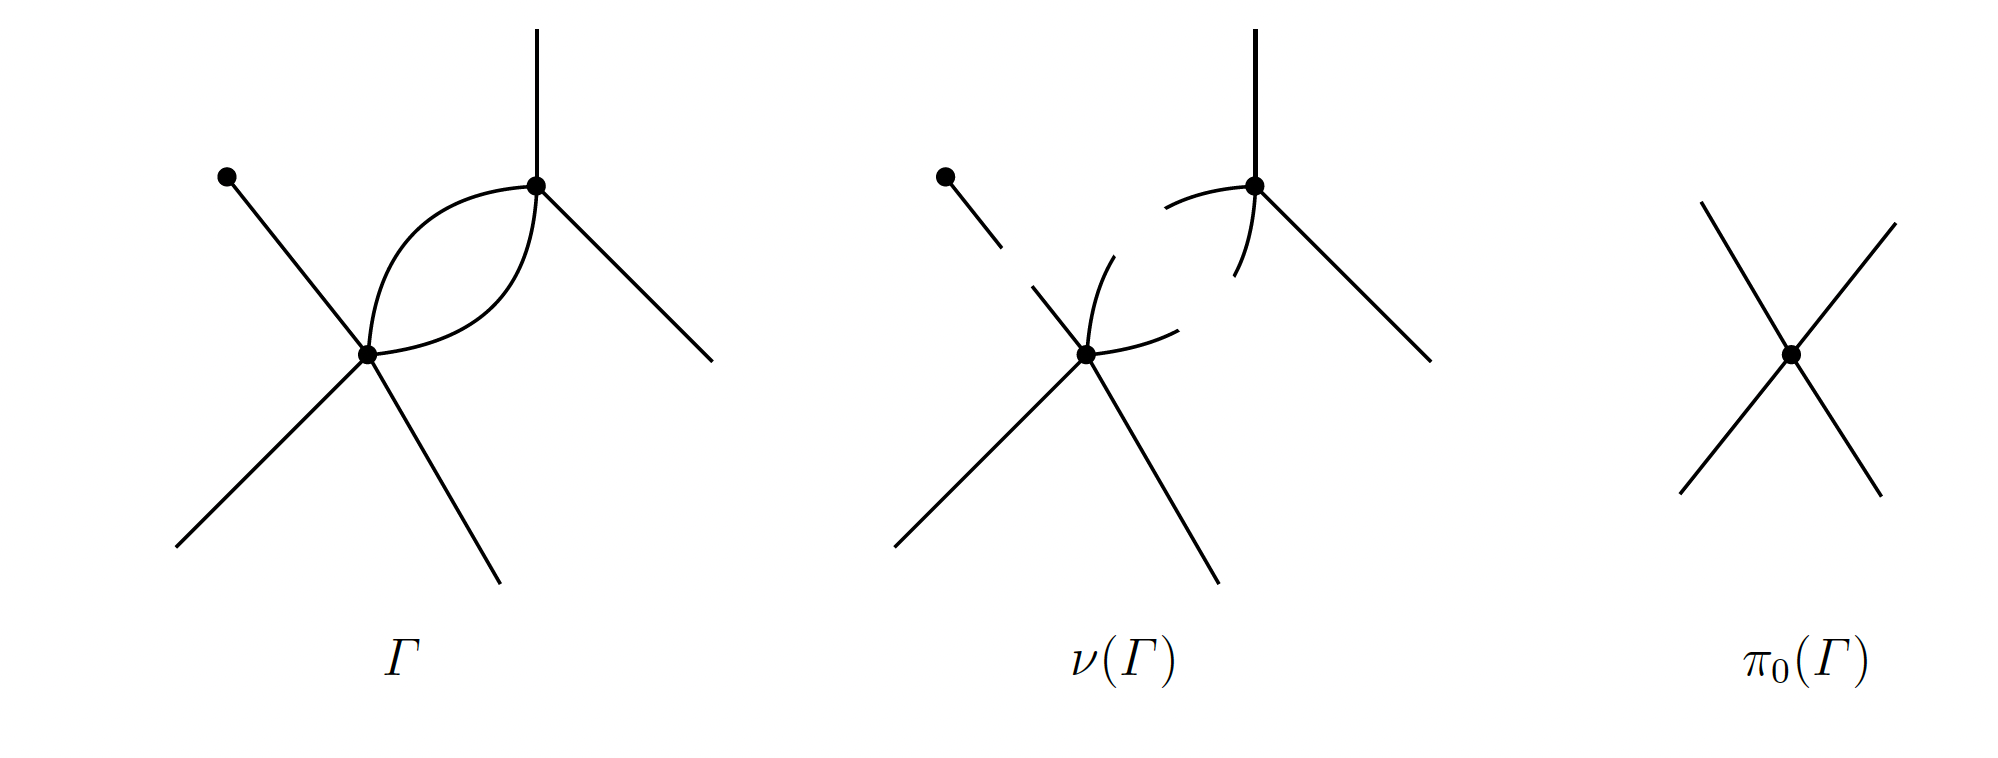
\includegraphics[width=0.8\textwidth]{graphs.png}$$

The category $\mathsf{Graphs}$ has as objects graphs which are finite disjoint unions of corollas. A morphism $\gamma_1 \to \gamma_2$ is given by an equivalence class of a graph $\Gamma$ together with isomorphisms $\phi_1 : \gamma_1 \to \nu(\Gamma)$ and $\phi_2 : \gamma_2 \to \pi_0(\Gamma)$; note that here $\phi_1$ and $\phi_2$ are morphisms of graphs in the above sense, but not morphisms in the category $\mathsf{Graphs}$ (which is named afters its morphisms). Two such triples $(\Gamma, \phi_1, \phi_2)$ and $(\Gamma', \phi'_1, \phi'_2)$ are equivalent if there exists an isomorphism $\psi : \Gamma \to \Gamma'$ satisfying $\phi'_1 = \nu(\psi) \circ \phi_1$ and $\phi_2 = \pi_0(\psi) \circ \phi'_2$. The composition $\Gamma_2 \circ \Gamma_1$ is defined by replacing the vertices of $\Gamma_2$ by the graph $\Gamma_1$, see below:
$$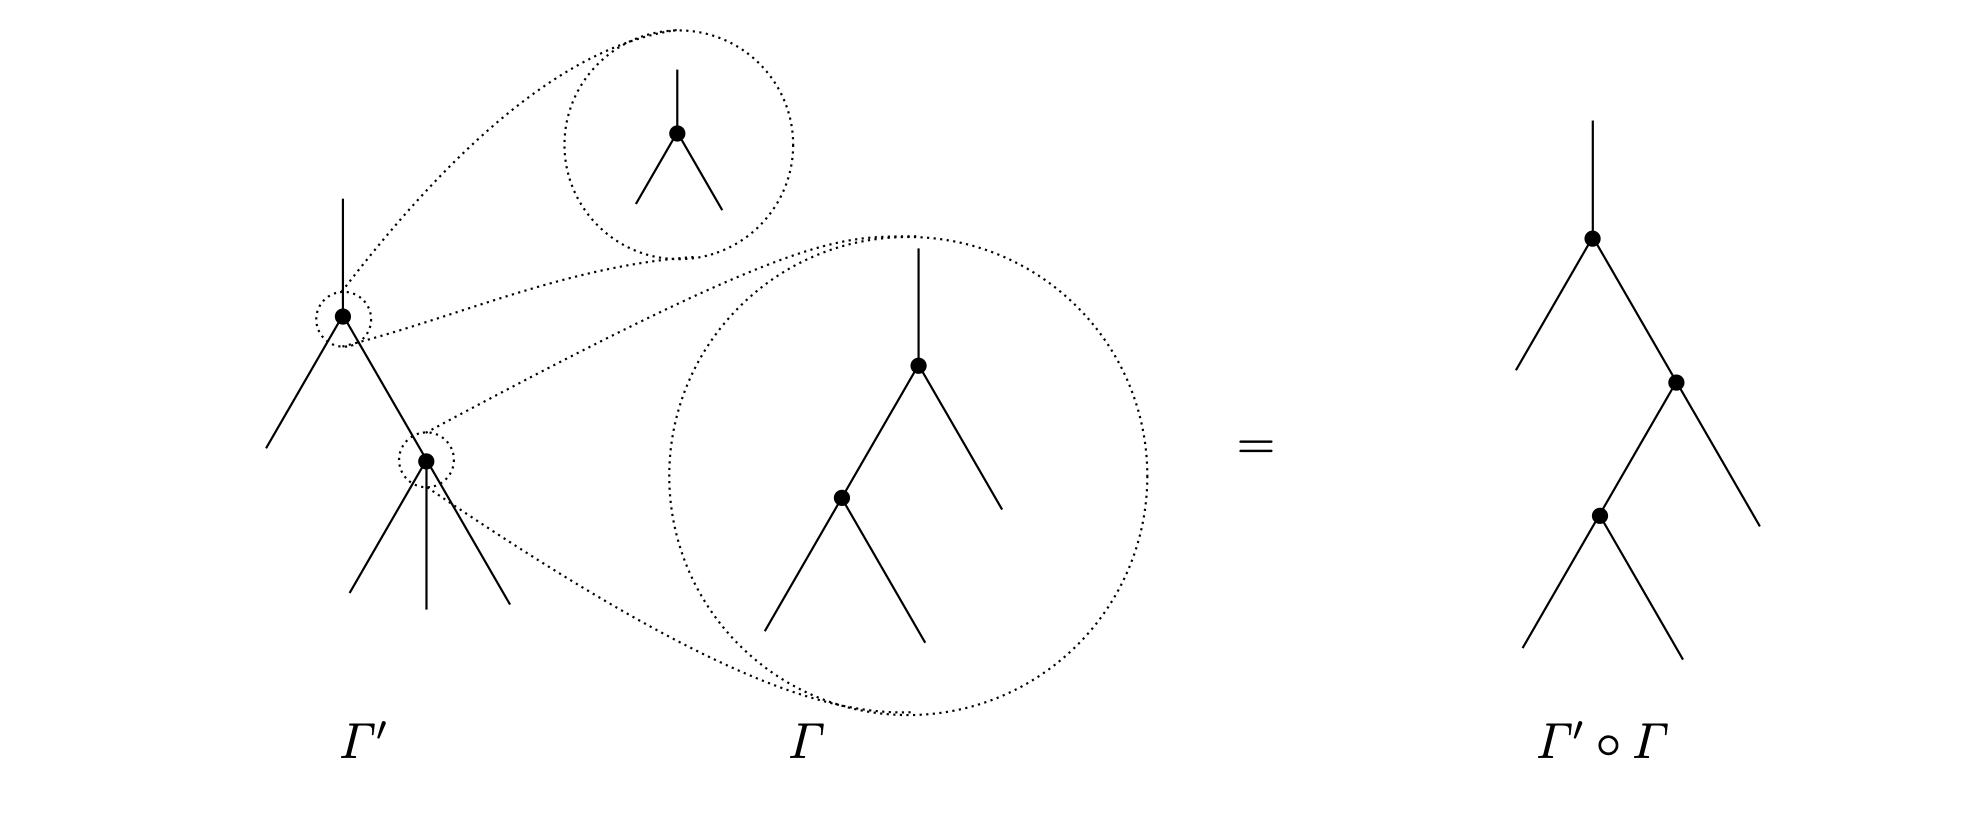
\includegraphics[width=0.9\textwidth]{composition.png}$$
We denote by $\mathsf{Forests}$ the subcategory of $\mathsf{Graphs}$ whose objects are those objects of $\mathsf{Graphs}$ which do not contain a corolla with zero legs and whose morphisms are forests, i.e.\ disjoint unions of contractible graphs.

Finally, we define the category $\mathsf{RForests}$ of \emph{rooted forests}: A \emph{rooted graph} is a graph $\Gamma$ equipped with a section $s : V(\pi_0(\Gamma)) \to \mathsf{Legs}(\Gamma)$ of the obvious map $\mathsf{Legs}(\Gamma) \to V(\pi_0(\Gamma))$, i.e.\ in each component of $\Gamma$ we distinguish an external leg that we refer to as the \emph{root}. Morphisms of rooted graphs are morphisms of the underlying graph which are compatible with the specified sections. Note that a rooted forest $\Gamma$ induces the structure of a rooted graph on $\nu(\Gamma)$ by declaring for every vertex the edge in the direction of the root of $\Gamma$ as the root of the vertex in $\nu(\Gamma)$. The category $\mathsf{RForests}$ is defined just like $\mathsf{Forests}$ with objects and morphisms replaced by their rooted version. There is a functor $\mathsf{RForests} \to \mathsf{Forests}$ which forgets the root.



We assume some familiarity with the theory of symmetric monoidal bicategories; we refer e.g. to [SP09, Chapter 2] for a detailed discussion and to [Lei98] for a short introduction (however without the treatment of monoidal structures). In particular, we rely on the following notions: By a \emph{bicategory} we mean a three-layered categorical structure with objects, 1-morphisms and 2-morphisms (sometimes also called 0-cells, 1-cells and 2-cells) in the weak sense. A \emph{morphism between bicategories} (sometimes also referred to as (weak) 2-functor) will just be called \emph{functor}. \emph{Symmetric monoidal functors} between symmetric monoidal bicategories are to be understood in a strong (not in any kind of lax) sense unless otherwise stated. In particular, a symmetric monoidal functor between symmetric monoidal bicategories comprises various sorts of coherence data subject to coherence conditions. We will briefly illustrate this after the next definition.


Let $\mathcal{M}$ be a symmetric monoidal bicategory. An \emph{operad} / \emph{cyclic operad} / \emph{modular operad}  in $\mathcal{M}$ is a symmetric monoidal functor $$\mathcal{O} : \mathsf{RForests} \ / \ \mathsf{Forests}  \ / \ \mathsf{Graph} \to \mathcal{M}$$ where we consider $\mathsf{RForests} \ / \ \mathsf{Forests}  \ / \ \mathsf{Graph}$ as a symmetric monoidal bicategory with only trivial 2-morphisms. See [MW, page 9] to see the equivalence with the classical definitions.

Let us emphasize that this defines operads \emph{without} an operadic identity. However, all operads appearing in this paper have operadic unit, and it will be important to correctly keep track of those. 




\subsection{The correspondence between groupoids and 1-homotopy types}

A 1-homotopy type is a topological space with $\pi_n(X,x_0)=0$ for all basepoints $x_0 \in X$. A connected 1-homotopy type is an asphereical space, aka an Eilenberg-MacLane space.


There is a diagram of categories and functors that we explain below:
$$\begin{tikzcd}
    \mathsf{Cat} \rar{N} \arrow[rr,bend left, "B"] & \mathsf{sSet} \rar{|-|} & \mathsf{Top}^{CW} \arrow[equals]{d} \\
  \mathsf{Gpd} \arrow[hook]{u}  \arrow[r,bend left, "N"]  & \mathsf{Kan}  \arrow[r,bend left, "|-|"]  \arrow[hook]{u} \arrow[l,bend left, "\Pi_1"] & \mathsf{Top}^{CW} \arrow[l,bend left, "Sing"] \arrow[ll,bend left, shift left=3, "\Pi"]
\end{tikzcd}$$
Here

\begin{itemize}
    \item $N$ is the nerve. It is a fully faithful functor.
    \item $|-|$ is the geometric realisation functor.
    \item $Sing$ is the singular functor; $Sing(X)$ is the simplicial sets with $Sing(X)_n$ the set of singular $n$-chains.
    \item $\Pi_1$ is the fundamental group of a Kan complex.
    \item  $B$ (defined as the composition) is the classifying space functor.
    \item $\Pi$ is the fundamental groupoid functor.
\end{itemize}


The main result is that up to homotopy we have that the the Sing - $|-|$ adjunction induces an equivalence $$ |-|:  \mathsf{Ho}(\mathsf{Kan}) \simeq \mathsf{Ho}(\mathsf{Top}^{CW}) : Sing$$
The key point is that restricting (composing) to groupoids induces an equivalence $$ B: \mathsf{Ho}(\mathsf{Gps}) \simeq \mathsf{Ho}(\mathsf{Top}^{CW}_{\leq 1}) : \Pi$$

In particular this means that a groupoid is the same thing as a 1-homotopy type; and a \textbf{connected groupoid }the same thing as an aspherical space.

A way to see this equivalence is the following: if $\C$ is a groupoid, $B \C = |N \C|$ is a disjoint union the $K(\pi,1)$'s. This is because every groupoid is a disjoint union of its connected components (a groupoid is connected is every object is connected through a morphism to every other object). Now $\C = \amalg_i \C_i$ with each $\C_i$ connected. Now for every $i$ take an object $X_i \in \C_i$, and let $\mathcal{G}_i$ be the full subcategory on that only object. That is, $\mathcal{G}_i$ is a 1-object groupoid aka a group, and the inclusion $\mathcal{G}_i \hookrightarrow \C_i$ is an equivalence for all $i$ as $\C_i$ is connected. So $\C \simeq \amalg_i \mathcal{G}_i$. It turns out that $B$ commutes with $\amalg$ so $$B \C \simeq \amalg B\mathcal{G}_i \simeq \amalg_i K(G_i,1 ).$$


\subsection{The (framed) little disc operad $E_n$ and $\mathsf{f}E_n$} 




First I need to recall a few things:
\begin{itemize}
    \item The (ordered) configuration space of a given space $X$ is $$\text{Conf}_n(X) := \{ (x_1, x_2, \ldots, x_n) \in X^n : x_i \neq x_j \text{ for all } i \neq j \}.$$
    \item The symmetric group $\mathfrak{S}_n$ naturally acts on $\text{Conf}_n(X)$. The unordered configuration space of $X $ is 
    $$ \text{UConf}_n(X) := \text{Conf}_n(X)/\mathfrak{S}_n ,$$ ie this is the space of sets of $n$ distint points.
    \item We have (more or less by def) isomorphisms
    $$ PB_n \cong \pi_1 (\text{Conf}_n(D^2))  \qquad , \qquad   B_n \cong \pi_1 (\text{UConf}_n(D^2)) ,$$
    where $B_n$ and $PB_n$ are the braid and pure braid group on $n$ strands, respectively.
    \item  These two spaces $\text{Conf}_n(D^2)$ and $\text{UConf}_n(D^2)$ are aspherical by a classic theorem by Fox-Neuwirth. Therefore (as they are connected) $$  B( PB_n) \simeq \text{Conf}_n(D^2)  \qquad , \qquad   B(B_n) \simeq \text{UConf}_n(D^2).  $$

\end{itemize}

There is a framed version of this story

\begin{itemize}
    \item The (ordered) framed configuration space of a given manifold $M$ is $$ \text{Conf}_n^{fr}(M):=  \{ ((x_1, f_1), (x_2, f_2), \ldots, (x_n, f_n)) \in (Fr(M))^n \mid x_i \neq x_j \text{ for all } i \neq j \}$$
    where $Fr(M)$ is the frame bundle of $M$.
    \item The symmetric group $\mathfrak{S}_n$ naturally acts on $\text{Conf}_n^{fr}(M)$. The unordered framed configuration space of $X $ is 
    $$ \text{UConf}_n^{fr}(M) := \text{Conf}_n^{fr}(M)/\mathfrak{S}_n .$$
    \item  We have (more or less by def) isomorphisms
    $$ PB_n^{fr} \cong \pi_1 (\text{Conf}_n^{fr}(D^2))  \qquad , \qquad   B_n^{fr} \cong \pi_1 (\text{UConf}^{fr}_n(D^2)) ,$$
    where $B_n^{fr}$ and $PB_n^{fr}$ are the framed braid and pure framed braid group on $n$ strands, respectively. That is, we have ribbons instead of strings.
    \item These spaces are again aspherical and then 
    $$  B( PB_n^{fr}) \simeq \text{Conf}^{fr}_n(D^2)  \qquad , \qquad   B(B_n^{fr}) \simeq \text{UConf}^{fr}_n(D^2).  $$
\end{itemize}





The \textbf{little $n$-disc operad} $E_n$ is a topological operad (ie an operad in the symmetric monoidal category of spaces) defined as $$ E_n(k) := \text{Emb}_{\text{rect}} (([0,1]^n)^{\amalg k}, [0,1]^n) $$ the space of rectilinear embeddings; see Example 1.8 in Heuts-Moerdijk for a precise definition. It is obvious that this space is isomorphic to $\text{Emb}_{\text{td}} ((D^n)^{\amalg k}, D^n)$ the space of embeddings that are obtained by a composition of translations and dilatations, and $D^n$ is the $n$-disc.

The \textbf{framed little $n$-disc operad} $\textsf{f}E_n$ is the topological operad defined as 
$$\textsf{f}E_n(k):= \text{Emb}_{\text{tdr}} ((D^n)^{\amalg k}, D^n)$$   the space of embeddings that are obtained by a composition of translations, dilatations and rotations. By ...... ????? ..... , the space $\text{Emb}_{\text{tdr}} ((D^n)^{\amalg k}, D^n)$ is in fact homotopy equivalent to the space $\text{Emb} ((D^n)^{\amalg k}, D^n)$ of all embeddings.\medskip

 \noindent \textbf{Key property:} Evaluation at the centre induces homotopy equivalences
$$  \text{Emb}_{\text{td}} ((D^n)^{\amalg k}, D^n) \to  \text{Conf}_k(D^n) $$ and 
$$  \text{Emb}_{\text{tdr}} ((D^n)^{\amalg k}, D^n) \to  \text{Conf}^{fr}_k(D^n) .$$

 \noindent \textbf{Upshot:}  $E_2(k)$ and $\textsf{f}E_2(k)$ are aspherical spaces, in particular we have $$ E_2(k) \simeq B(PB_k) \qquad , \qquad   \textsf{f}E_2(k) \simeq B(PB_k^{fr}). $$
In particular, by the equivalence between connected groupoids and aspherical spaces, we can regard $\textsf{f}E_2$ and $E_2$ as operads in groupoids, not in spaces.
 




\subsection{Disc algebras vs. framed $E_n$-algebras} 


I will describe here roughly the (2,1)-categorical version; there is also an $\infty$-categorical ones.


Let $\mathsf{Disc}_n$  the symmetric monoidal $(2,1)$-category with objects disjoint union of oriented disks and hom groupoids orientation-preserving embeddings with isotopies, with disjoint union as monoidal product. If $\C$ is a symmetric monoidal $(2,1)$-category, a \textbf{disk algebra }is a symmetric monoidal functor $\mathsf{Disc}_n \to \C$.

There is a framed variant of this story:  $\mathsf{Disc}_n^{fr}$  the symmetric monoidal $(2,1)$-category with objects disjoint union of framed (=choice of trivialisation of the tangent bundle)  disks and arrows  embeddings equipped with a compatibility of framings (see Tanaka's notes for a precise statement), with disjoint union as monoidal product. If $\C$ is a symmetric monoidal $(2,1)$-category, a \textbf{framed disk algebra} is a symmetric monoidal functor $\mathsf{Disc}_n^{fr} \to \C$.\medskip


\noindent \textbf{Theorem.} The following three pieces of data are equivalent (inducing equivalences of the corresponding categories):
\begin{enumerate}
    \item A 2-disk algebra in $\Rexf$,
    \item A $\Rexf$-valued framed $E_2$-algebra,
    \item A balanced monoidal category in $\Rexf$.
\end{enumerate}
($\Rexf$ can be replaced by something more general like $LFP_c$).

The equivalence between 1 and 3 is explained with detail in Theorem 3.2 of Brochier's notes "Factorisation homology of braided tensor categories": for a functor $F: \mathsf{Disc}_n \to \Rexf$ then $\cA:=F(D^2)$ is a balanced monoidal category.

I want to focus on the equivalence 1 - 2. The key word is \textbf{envelope construction} which is nothing but the adjunction between operads and PROPs (= symm mon cat gen by a single object)
$$F: Operads \rightleftarrows PROPs :U$$
and more concretely how to construct a symmetric monoidal category out of an operad. One builds the ``free PROP'' aka envelope of an operad putting together the trees; the right adjoint uses simply one output, so that's kinda a forgetful.

In the groupoid-valued setting, the adjunction reads
$$  F: \mathsf{Op}(\mathsf{Gpd})  \rightleftarrows  (2,1)-\mathsf{PROPs} :U $$
Obviously the endomorphism operad $\text{End}_\cA$ can be viewed as the forgetful $\text{End}_\cA=U(\widetilde{\text{End}_\cA})$ (restriction) of a (2,1)-PROP $\widetilde{\text{End}_\cA}$ with  $\widetilde{\text{End}_\cA}(n,m):= \Rexf(\cA^{\boxtimes n}, \cA^{\boxtimes m})$. The adjunction says that there is an equivalence
$$ \text{Hom}_{PROP}(F(\mathsf{f}E_2),\widetilde{\text{End}_\cA} ) \simeq \text{Hom}_{Op}(\mathsf{F} E_2,\text{End}_\cA ) .$$
The RHS are precisely $\Rexf$-valued framed $E_2$-algebras. Now the point is that the LHS are exactly the same as framed 2-disc algebras in $\Rexf$, ie symm mon functors $\mathsf{Disc}_2 \to \Rexf$. Modifying the target is easy: $\widetilde{\text{End}_\cA}$ is a full subcat of $\Rexf$ so it changes nothing as $\mathsf{Disc}_2$ is generated by a single object (namely the 2-disc). So everything amounts to showing that $F(\mathsf{f}E_2) \simeq \mathsf{Disc}_2 $ as (2,1)-categories.

Here one has to remember from the previous subsection that

$$ \mathsf{f} E_2 (n) =  \text{Emb}_{\text{tdr}} ((D^2)^{\amalg n}, D^2) \simeq \text{Emb} ((D^2)^{\amalg n}, D^2), $$
so viewed in groupoids, one applies by the correspondence explained above the fundamental groupoid functor, 
$$ \mathsf{f} E_2 (n) = \Pi \text{Emb} ((D^2)^{\amalg n}, D^2) $$
as a groupoid-valued operad. If we then consider the free (2,1)-PROP, that is, the thing obtained by concatenating trees, then we get that
$$F( \mathsf{f} E_2) (n,m) = \Pi \text{Emb} ((D^2)^{\amalg n}, (D^2)^{\amalg m}), $$ that is $\mathsf{Disc}_2 $.









There is  also an ``unframed'' version of this theorem:



\noindent \textbf{Theorem.} The following three pieces of data are equivalent (inducing equivalences of the corresponding categories):
\begin{enumerate}
    \item A framed 2-disk algebra in $\Rexf$,
    \item A $\Rexf$-valued $E_2$-algebra,
    \item A braided monoidal category in $\Rexf$.
\end{enumerate}


\subsection{The cyclic and modular endomorphism operad}

(Mostly taken from Woike's reflection equivariance paper)\medskip

Classically, an algebra $X$ over an operad $\mathcal{O}$ is an operad map  $$\mathcal{O} \to \mathrm{End}_X$$ to the endomorphism operad of the underlying object of the algebra $X$; recall that $\mathrm{End}_X(n)= \mathrm{Hom}(X^{\otimes n}, X)$. If $X$ was a vector space for instance, in order to make this endomorphism operad cyclic (or more genrally modular), ie to exchage a copy of $X$ to the target and the one from the target to the source, or to pair up two copies of $X$, we'd need an identification between $X$ and its dual aka a non-deg pairing in $X$. We do this next in general (with $\cA$ instead of $X$ as we're thinking of a symm mon bicat).


In order to generalize this to cyclic and modular operads, the endomorphism operad needs to be made modular (and therefore in particular cyclic). This is done in [MW23a, Section 2] for the bicategorical case, following the principles of [GK95, GK98, Cos04]: First we recall the notion of a \textbf{non-degenerate symmetric pairing} $\kappa : \mathcal{A} \boxtimes \mathcal{A} \to \mathcal{I}$ on an object $\mathcal{A}$ in a symmetric monoidal bicategory $\mathcal{S}$ with monoidal product $\boxtimes$ and monoidal unit $\mathcal{I}$, where
\begin{itemize}
    \item \textit{non-degeneracy} means that $\kappa$ exhibits $\mathcal{A}$ as its own dual in the homotopy category of $\mathcal{S}$, that is, there is a coevaluation object $\Delta : \mathcal{I} \to \mathcal{A} \boxtimes \mathcal{A}$ that together with $\kappa$ satisfies the zigzag identities up to isomorphism. 
    \item and \textit{symmetry} means that $\kappa$ is a homotopy fixed point in $\mathcal{S}(\mathcal{A} \boxtimes \mathcal{A}, \mathcal{I})$ with respect to the $\mathbb{Z}_2$-action coming from the symmetric braiding of $\mathcal{S}$.
\end{itemize}
Thanks to the non-degenerate symmetric pairing, we can define a symmetric monoidal functor $$\mathsf{End}_{\mathcal{A}, \kappa}: \mathsf{Graphs} \to \mathsf{Cat}$$ sending a corolla $T$ to the morphism category $$\mathsf{End}_{\mathcal{A}, \kappa}(T):=\mathcal{S}(\mathcal{A}^{\boxtimes \mathsf{Legs}(T)}, \mathcal{I})$$ from the unordered monoidal product $\mathcal{A}^{\boxtimes \mathsf{Legs}(T)}$ of $\mathcal{A}$ over the set $\mathsf{Legs}(T)$ of legs of $T$ to the monoidal unit $\mathcal{I} \in \mathcal{S}$. This $\mathsf{Cat}$-valued modular operad is the \textit{modular endomorphism operad} of $(\mathcal{A}, \kappa)$ and denoted by $\mathsf{End}_{\mathcal{A}, \kappa}$.

If $\mathcal{O}$ is a $\mathsf{Cat}$-valued modular operad $\mathcal{O} :\mathsf{Graphs} \to \mathsf{Cat}$, an \textit{$\mathcal{S}$-valued  modular $\mathcal{O}$-algebra}  is now defined as an object $\mathcal{A}$ in $\mathcal{S}$  with a non-degenerate symmetric pairing $\kappa$ plus a map $\mathcal{O} \to \mathsf{End}_{\mathcal{A}, \kappa}$ of modular operads (aka a symm mon nat transf). A \textit{cyclic algebra} is defined analogously. Both cyclic and modular algebras over a fixed cyclic or modular operad, respectively, with values in a symmetric monoidal bicategory form themselves bicategories in which all morphisms turn out to be invertible, i.e.\ they form 2-groupoids [MW23a, Proposition 2.18].


\paragraph{Unpacking the definition}
Let us partly unpack the definition of a $\Rexf$-valued modular $\mathcal{O}$-algebra (all of this is worked out in detail in [MW23a, Section 2.5] where the dual case of $\mathsf{Lex}^f$ is treated): It has an underlying object $\mathcal{A} \in \mathsf{Rex}^f$, i.e.\ a finite category, and a non-degenerate symmetric pairing $\kappa : \mathcal{A} \boxtimes \mathcal{A} \to \mathsf{vect}$. By virtue of right exactness, we have
$$ \Rexf(\cA \boxtimes \cA , \mathsf{vect}) \simeq (\cA \boxtimes \cA)^{op} \boxtimes    \mathsf{vect} \simeq  \cA^{op} \boxtimes \cA^{op} \simeq \Rexf (\cA, \cA^{op})$$
(here we have used the Eilenberg-Watts theorem) ie $\kappa$ determines an equivalence $D : \mathcal{A} \to \mathcal{A}^{\mathrm{op}}$ via $\kappa(X, Y) = \mathcal{A}(X, DY)^*$, and the symmetry of $\kappa$ induces an isomorphism $D^2 \simeq \mathrm{id}_{\mathcal{A}}$. The coevaluation is a right exact functor $\Delta : \mathsf{vect} \to \mathcal{A} \boxtimes \mathcal{A}$ and is hence (again by the Eilenberg-Watts theorem) an object in $\mathcal{A} \boxtimes \mathcal{A}$ given by the end
\[
\Delta = \int_{X \in \mathcal{A}} D X \boxtimes X;
\]
we refer to [FSS20] for an introduction to (co)ends in finite linear categories. Moreover, the structure of a modular $\mathcal{O}$-algebra on $\mathcal{A}$ provides us for each operation $o \in \mathcal{O}(T)$ for a corolla $T$ with a right exact functor $\mathcal{A}_o : \mathcal{A}^{\boxtimes \mathsf{Legs}(T)} \to \mathsf{vect}$. If $T \in \mathsf{Graphs}$ is not connected, i.e.\ $T = \coprod_{l \in L} T(l)$ with corollas $T(l)$, then to $o = (o_l)_{l \in L} \in \mathcal{O}(T) \simeq \prod_{l \in L} \mathcal{O}(T(l))$ the modular algebra associates the family of right exact functors $(\mathcal{A}_{o_l})_{l \in L}$; it gives us also a right exact functor $\bigoplus_{l \in L} \mathcal{A}_{o_l} \to \mathsf{vect}$ (by abuse of notation, we will not distinguish between these two objects). The data of a modular algebra includes also the compatibility with composition: Suppose that a morphism $\Gamma: T \to T'$ glues two legs (of $T$) together; that is, $\Gamma$ is like the leftmost $\Gamma'$ picture above if the legs belong to different corollas, or $\Gamma$ is the result of taking a given corolla $T$ and glue two legs (and then $T'$ is just $T$ minus the two legs that were glued).

Denote by $o' \in \mathcal{O}(T')$ the image of some $o \in \mathcal{O}(T)$ under the operadic composition $\mathcal{O}(\Gamma) : \mathcal{O}(T) \to \mathcal{O}(T')$. Then we obtain an isomorphism of right exact functors between $\mathcal{A}_{o'}$ and $\mathcal{A}_o$, but with $\Delta$ inserted into the two arguments of $\mathcal{A}_o$ corresponding to the legs that are glued together, i.e.
\begin{equation}
\mathcal{A}_{o'} \simeq \mathcal{A}_o(\dots, \Delta', \dots, \Delta'', \dots) \tag{2.2}
\end{equation}
with Sweedler notation $\Delta = \Delta' \boxtimes \Delta''$ for the coevaluation object (as usual, the notion does not imply that $\mathcal{A}$ is a pure tensor). In some contexts, (2.2) is called \textit{excision}.




\subsection{Classifications of cyclic and modular algebras}

The classical result:
$$ \Alg (\mathsf{f}E_2, \Rexf) \simeq \text{balanced monoidal categories in } \Rexf.$$

The intermediate result:
$$  \CycAlg (\As, \Rexf) \simeq \ModAlg(\OSurf, \Rexf) \simeq \text{pivotal GV-categories in } \Rexf.      $$
(for these we have used
$$\OSurf_{| g=0} \simeq \As \qquad , \qquad  \Hbdy_{|g=0} \simeq \mathsf{f}E_2$$

The classification of $\Rexf$-valued cyclic framed $E_2$-algebras:

$$ \CycAlg (\mathsf{f}E_2, \Rexf) \simeq  \ModAlg (\Hbdy, \Rexf) \simeq \text{ribbon GV-categories in } \Rexf$$
(a modular $\Hbdy$-algebra is called an ansular functor).




We also have $$\Surf_{| g=0} \simeq \mathsf{f}E_2,$$
ie $\mathsf{f}E_2$ is the ``cyclic operad of genus zero surfaces''

\subsection{Modular functors}




Cyclic framed $E_2$-algebra = genus zero modular functor.




\section{Factorisation homology}


\subsection{Definition}


\begin{equation}\label{eq:FH}
\begin{tikzcd}
\mathsf{Disc} \rar{\cA} \arrow[hook]{d}[swap]{\iota} & \Rexf \\
\mathsf{Surf}  \arrow[dashed]{ur}[swap]{\int_{(-)} \cA}  &
\end{tikzcd}
\end{equation}


\subsection{Properties}


\begin{itemize}
    \item We have $\int_{D^2} \cA \simeq \cA$, the equivalence being induced by any of the universal arrows $\cA \to \int_{D^2} \cA $ coming from the description of the homotopy colimit. This is true by construction: factorisation homology being a homotopy left Kan extension along an embedding means that the diagram \eqref{eq:FH} is actually commutative up to isomorphism. Since the image of the 2-disc under $\cA$ is $\cA$ as category, this yields the equivalence.
\end{itemize}


\subsection{Quantum structure sheaf or distinguished object}

Factorization homology is a \emph{canonically pointed} theory in the following sense: for a surface $\Sigma$, the unique embedding $\emptyset \hookrightarrow \Sigma$ induces a functor $$ \cat{O}_\Sigma: \mathsf{vect} \simeq \int_{\emptyset} \cA \to \int_\Sigma \cA  .$$ This functor produces a distinguished object in $\int_\Sigma \cA$, namely the image of the 1-dimensional vector space, $\cat{O}_{\cA, \Sigma} := \cat{O}_\Sigma (\Bbbk)$, that is called the \emph{quantum structure sheaf} in "Integrating Quantum groups".

Alternatively, $\cat{O}_{\cA, \Sigma}$ can be defined in a different way (up to isomorphism):  as the image of the monoidal unit $\mathbf{1}$ of $\cA$ under any of the universal functors $\cA \to \int_\Sigma \cA$  (a leg of the colimit cone) for any embedding $D^2 \hookrightarrow \Sigma$. 


To see that the two descriptions agree, one argues as follows: the first observation is that if they agree for a given embedding then it is independent on the chosen embedding. Now the second observation is that it suffices to check this for the disc $D^2$, this is because no matter for what embedding $D^2 \hookrightarrow \Sigma$ we have a commutative diagram of embeddings
$$\begin{tikzcd}
  &  \emptyset \arrow{dl} \arrow{dr} & \\
  D^2 \arrow{rr} & & \Sigma
\end{tikzcd}$$
since $\emptyset$ is initial; and then we get a commutative diagram (up to iso)
$$\begin{tikzcd}
  &  \mathsf{vect} \arrow{dl} \arrow{dr} & \\
  \int_{D^2} \cA  \arrow{rr} & & \int_\Sigma \cA
\end{tikzcd}$$
which means that any embedding $D^2 \hookrightarrow \Sigma$ induces a functor $\int_{D^2} \cA \to \int_\Sigma \cA$ that maps the distinguished object to the distinguished object. Therefore it suffices to check that under the equivalence $\int_{D^2} \cA \simeq \cA$, the distinguished object $\mathcal{O}_{\cA,D^2}$ corresponds precisely with the monoidal unit of $\cA$.

Now the key is that a balanced monoidal category is a different name for a framed $E_2$-algebra aka a 2-disc algebra, that is a functor $\mathsf{Disk} \to \Rexf$. The monoidal unit is given by the canonical embedding $\emptyset \hookrightarrow D^2$ inducing a map $\mathsf{vect}\to \cA$ which maps the base field to the monoidal unit. By the commutativity of \eqref{eq:FH} we have that the functors $\mathsf{vect}\to \cA$ and $\mathsf{vect}\to \int_{D^2} \cA$ must be isomorphic (up to the equivalence in the target). Ie that $\mathcal{O}_{\cA,D^2} \cong \mathbf{1}$ viewed in $\cA$.



The same type of argument says that if $\amalg_k D^2 \hookrightarrow \Sigma$ is an embedding, with universal functor $\cA^{\boxtimes k} \to \int_\Sigma \cA$, and that embedding factors through a larger disc, ie there is a diagram 
$$\begin{tikzcd}
  &  \amalg_k D^2 \arrow{dl} \arrow{dr} & \\
  D^2 \arrow{rr} & & \Sigma
\end{tikzcd}$$
then the universal functor $\cA^{\boxtimes k} \to \int_\Sigma \cA$ factors through the monoidal product of $\cA$, ie there is  a commutative diagram (up to iso)
$$\begin{tikzcd}
    \cA^{\boxtimes k}  \rar \dar[swap]{\otimes^k} &  \int_\Sigma \cA \\
    \cA \arrow[dashed]{ur} &
\end{tikzcd}$$


\subsection{Moduli algebra}


This is $A_\Sigma := \underline{\mathsf{End}}(\mathcal{O}_{\mathcal{A}, \Sigma})$. Not to be confused with $\mathcal{F}_{\mathcal{A}} := \otimes\underline{\mathsf{End}}(\mathbf{1})$ (the \textit{reflection equation algebra}) or with $a_P := \mathcal{F}_{\mathcal{A}} ^{\otimes n}$ where $P$ is a pattern of rank $n$.


\subsection{Skein algebra (categorical version))}

This is the endomorphism algebra $$  \mathsf{SkAlg}_\cA (\Sigma):= \mathsf{End}_{\int_{\Sigma} \cA} (\mathcal{O}_{\mathcal{A}, \Sigma}). $$







	
\section{Module categories}


In this section, we review some categorical notions that will play a major role in the present article. Without further comment, all categories  will be assumed to \emph{$\Bbbk$-linear} over a fixed algebraically closed  field $\Bbbk$, that is, enriched over the symmetric monoidal category  of vector spaces over $\Bbbk$, and all functors and natural transformations will be assumed to be $\Bbbk$-linear as well.


\subsection{Finite categories}

Following \cite{etingofostrik}, a \emph{finite category} is an abelian category $\mathcal{A}$ such that
\begin{enumerate}[label=(\roman*)]\itemsep0em 
  \item the hom-vector spaces are finite-dimensional,
  \item every object has finite length,
  \item there are finitely many isomorphisms classes of simple objects,
  \item $\mathcal{A}$ has enough projectives.
\end{enumerate}
It is well-known that an abelian category is finite if and only if it equivalent to the category $A$-$\mathsf{mod}$ of finite-dimensional modules over a finite-dimensional algebra $A$. Therefore, a given finite category determines the Morita equivalence class of a finite-dimensional algebra.

Recall that abelian categories are \emph{finitely (co)complete}, that is, they have all finite (co)limits. A functor $F: \mathcal{C} \to \mathcal{D}$ between abelian categories is \emph{left} (resp. \emph{right}) \emph{exact} if it preserves finite limits (resp. colimits).  Alternatively, $F$ is left (resp. right) exact if and only if it preserves kernels (resp. cokernels). The functor $F$ is \emph{exact} if it is left and right exact.

The following version of the Eilenberg-Watts theorem will be heavily used in the sequel:

\begin{lemma}[{\cite[Corollary 2.3]{fss}}]\label{lem:left_exact=right_adjoint}

Let $F,G: \mathcal{A} \to \mathcal{B}$ be functors between finite categories. Then the following are equivalent:
\begin{enumerate}\itemsep0em 
\item[(L1)] $F$ is left exact,
\item[(L2)] $F$ is right-adjoint,
\end{enumerate}
and if $\mathcal{B} = \mathsf{vect}$ the category of finite-dimensional vector spaces, then they are likewise equivalent to
\begin{enumerate}
\item[(L3)] $F$ is representable, $F \cong \mathsf{Hom}_{\mathcal{A}}(X,-)$ for some object $X \in \mathcal{A}$.
\end{enumerate}
Similarly, the following are equivalent:
\begin{enumerate}\itemsep0em 
\item[(R1)] $G$ is right exact,
\item[(R2)] $G$ is left-adjoint,
\end{enumerate}
and if $\mathcal{B} = \mathsf{vect}$, then they are equivalent to
\begin{enumerate}
\item[(R3)] $G$ is ``dually representable'', $G \cong \mathsf{Hom}_{\mathcal{A}}(-,X)^*$ for some object $X \in \mathcal{A}$.
\end{enumerate}
\end{lemma}


\subsection{Finite tensor categories}

A finite category $\mathcal{A}$ equipped with a rigid bilinear monoidal  product  with simple unit is called a \emph{finite tensor category}~\cite{etingofostrik}. The left and right rigidity induce strong monoidal functors
\begin{equation}\label{eq:duality_functors}
(-)^\vee: \mathcal{A} \to \mathcal{A}^{\mathsf{op}, \mathsf{rev}}  \qquad , \qquad ^{\vee}(-): \mathcal{A}^{\mathsf{op} , \mathsf{rev}}\to \mathcal{A} 
\end{equation}
respectively, 
which are mutually quasi-inverses. Here for a monoidal category $\mathcal{C} = (\mathcal{C} , \otimes, \mathbbm{1})$, we have put 
$$ \mathcal{C}^{\mathsf{op}} = (\mathcal{C}^{\mathsf{op}}, \otimes, \mathbbm{1})  \qquad , \qquad  \mathcal{C}^{\mathsf{rev}} = (\mathcal{C}, \otimes^{\mathsf{rev}}, \mathbbm{1}) \qquad , \qquad \mathcal{C}^{\mathsf{op}, \mathsf{rev}} = (\mathcal{C} ^{\mathsf{op}})^{\mathsf{rev}} $$ with $
X \otimes^{\mathsf{rev}} Y := Y \otimes X$.


In a finite tensor category $\mathcal{A}$, we have adjunctions (e.g. \cite[\S 2.7]{shimizuunimodular})
\begin{equation}\label{eq:adjunctions_duals_ftc}
X^\vee \otimes(-)\dashv X\otimes(-)\dashv {}^\vee X\otimes(-)\qquad , \qquad (-)\otimes {}^\vee X\dashv(-)\otimes X\dashv(-)\otimes X^\vee 
\end{equation}
for every object $X \in \mathcal{A}$, so by  \cref{lem:left_exact=right_adjoint} the monoidal product bifunctor $\otimes : \mathcal{A} \times \mathcal{A} \to \mathcal{A} $ is exact in each variable.


\subsection{Finite module categories}\label{subsec:finite_mod_cats}

Let $\mathcal{C}$ be a monoidal category. A \emph{left $\mathcal{C}$-module structure} on a category $\mathcal{M}$ is the data of an action bifunctor $\ogreaterthan : \mathcal{C} \times \mathcal{M} \longrightarrow \mathcal{M} $ and a family of natural isomorphisms
$$ \mathbbm{1}\ogreaterthan M \cong M \qquad , \qquad  (X \otimes Y)\ogreaterthan  M \cong X \ogreaterthan (Y \ogreaterthan M)  $$ satisfying a pentagon and triangle axioms similar to those for monoidal categories, see \cite[\S 7.1]{egno} for details (a \emph{right $\mathcal{A}$-module category} is defined analogously with an action functor $\olessthan : \mathcal{M} \times \mathcal{C} \longrightarrow \mathcal{M}$).  Similarly, an \emph{$\mathcal{A}$-module functor} $F: \mathcal{M} \longrightarrow \mathcal{N}$ between $\mathcal{A}$-module categories is a functor together with natural isomorphisms $$ F(X \ogreaterthan M) \cong F(X) \ogreaterthan M   $$ satisfying similar axioms, cf.  \cite[\S 7.2]{egno}.

If $\mathcal{A}$ is a finite tensor category, a finite category $\mathcal{M}$ equipped with a  $\mathcal{A}$-module structure is called a \emph{finite $\mathcal{A}$-module category} if the functors $- \ogreaterthan M : \mathcal{A} \longrightarrow \mathcal{M}$  are right exact for any $M \in \mathcal{M}$. Similarly to the case of finite tensor categories, we have adjunctions
\begin{equation}\label{eq:adjunctions_action_functor}
X^\vee \ogreaterthan (-)\dashv X\ogreaterthan (-)\dashv {}^\vee X\ogreaterthan(-)
\end{equation} 
so again  \cref{lem:left_exact=right_adjoint} implies that the functor $X \ogreaterthan - : \mathcal{M} \longrightarrow \mathcal{M}$ is always exact for any $X \in \mathcal{A}$.

\subsection{Internal homs}\label{subsec:internal_homs}

Let $\mathcal{A}$ be a finite tensor category and $\mathcal{M}$ a finite $\mathcal{A}$-module category. For every $M \in \mathcal{M}$, the functor $-	 \ogreaterthan M$ has a right-adjoint by \cref{lem:left_exact=right_adjoint}, that we denote by $\underline{\mathsf{Hom}}(M,-): \mathcal{M} \longrightarrow \mathcal{A}$. By definition, there are linear isomorphisms
\begin{align}\label{eq:internal_hom_adj}
\mathsf{Hom}_{\mathcal{M}}(X \ogreaterthan M,N) \cong \mathsf{Hom}_\mathcal{A} (X, \underline{\mathsf{Hom}}(M,N)) 
\end{align}
natural in $X \in \mathcal{A}$ and $N \in \mathcal{M}$.
According to the parametrized adjunction theorem \cite[Theorem IV.7.3]{maclane}, the right adjoints in this family of adjunctions assemble in a unique way into a bifunctor
\begin{equation}\label{eq:internal_hom_functor}
\underline{\mathsf{Hom}}:\mathcal{M}^{\mathsf{op}} \times \mathcal{M} \longrightarrow \mathcal{A}
\end{equation}
such that the isomorphism \eqref{eq:internal_hom_adj} is natural in the three variables. We call \eqref{eq:internal_hom_functor} the \emph{internal hom functor}. This bifunctor is, just like the hom functor,  left exact in both variables: indeed by definition $\underline{\mathsf{Hom}}(M,-)$ is right-adjoint to $- \ogreaterthan M$, and the isomorphisms
\begin{align*}
\mathsf{Hom}_{\mathcal{M}^\mathsf{op}}(X^\vee \ogreaterthan N,M) \overset{\eqref{eq:adjunctions_action_functor}}  {\cong} \mathsf{Hom}_{\mathcal{M}^\mathsf{op}}( N,X \ogreaterthan M) \cong  \mathsf{Hom}_{\mathcal{M}}( X \ogreaterthan M, N)  \cong \mathsf{Hom}_\mathcal{A} (X, \underline{\mathsf{Hom}}(M,N)) 
\end{align*}
show that  $\underline{\mathsf{Hom}}(-,N)$ is right-adjoint to $(-)^\vee \ogreaterthan N$. Once again we conclude  by \cref{lem:left_exact=right_adjoint}. 


We also record that for objects $X,Y \in \mathcal{A}$ and $M,N \in \mathcal{M}$ there is a natural isomorphism
\begin{equation}\label{eq:iso_2.15}
\underline{\mathsf{Hom}}(X \ogreaterthan M, Y \ogreaterthan N) \cong Y \otimes \underline{\mathsf{Hom}}(M,N) \otimes X^\vee,
\end{equation}
see \cite[Lemma 7.9.4]{egno} or \cite[(2.15)]{shimizuunimodular}.

The aforementioned internal homs can be used to equip $\mathcal{M}$ with a structure of $\mathcal{A}$-enriched category: for $L,M,N \in \mathcal{M}$ there is a composition map
\begin{equation}\label{eq:enriched_composite}
\underline{\circ}_{L,M,N} := \underline{\mathrm{ev}}_{M,N} \circ (\mathrm{id} \ogreaterthan \underline{\mathrm{ev}}_{L,M}) : \underline{\mathsf{Hom}}(M,N)\otimes \underline{\mathsf{Hom}}(L,M)\longrightarrow \underline{\mathsf{Hom}}(L,N)
\end{equation}
where $\underline{\mathrm{ev}}_{M,N} : \underline{\mathsf{Hom}}(M,N) \ogreaterthan M \longrightarrow N$ is the counit of the adjunction  \eqref{eq:internal_hom_adj}. The identity arrow $$ \underline{\mathrm{id}}_M:  \mathbbm{1} \longrightarrow \underline{\mathsf{End}}(M):= \underline{\mathsf{Hom}}(M,M) $$  is the morphism corresponding to the isomorphism $\mathbbm{1} \ogreaterthan M \cong M$ under the isomorphism \eqref{eq:internal_hom_adj}. In particular, for any object $M \in \mathcal{M}$, we have that $\underline{\mathsf{End}}(M)$ is an algebra object in $\mathcal{A}$, and for any  $N \in \mathcal{M}$ the object $\underline{\mathsf{Hom}}(M,N)$ is a right $\underline{\mathsf{End}}(M)$-module in $\mathcal{A}$ with structure morphism given by \eqref{eq:enriched_composite} with $L=M$.

We denote by $\mathsf{mod}_\mathcal{A}{\text -}\underline{\mathsf{End}}(M)$ the category of right $\underline{\mathsf{End}}(M)$-modules in $\mathcal{A}$. It is readily verified that the monoidal product $\otimes : \mathcal{A} \times \mathcal{A} \longrightarrow \mathcal{A}$ restricts to a functor  $\mathcal{A} \times \mathsf{mod}_\mathcal{A}{\text -}\underline{\mathsf{End}}(M)\longrightarrow \mathsf{mod}_\mathcal{A}{\text -}\underline{\mathsf{End}}(M)$ turning it into  a left $\mathcal{A}$-module category. In particular, $\underline{\mathsf{Hom}}(M,-)$ restricts to a functor
$$\underline{\mathsf{Hom}}(M,-): \mathcal{M} \longrightarrow  \mathsf{mod}_\mathcal{A}{\text -}\underline{\mathsf{End}}(M)  $$ for which the isomorphisms \eqref{eq:iso_2.15} make it an $\mathcal{A}$-module functor.

\begin{theorem}[Monadicity for module categories, e.g. {\cite[\S 7.10]{egno}}]\label{thm:monadicity_thm}
Let $M \in \mathcal{M}$. Then the functor $$\underline{\mathsf{Hom}}(M,-): \mathcal{M} \longrightarrow  \mathsf{mod}_\mathcal{A}{\text -}\underline{\mathsf{End}}(M)  $$ is an equivalence of left $\mathcal{A}$-module categories if and only if $M$ is an $\mathcal{A}$-progenerator. Moreover, such an object always exists.
\end{theorem}

In the statement above, an object $M \in \mathcal{M}$ is an \emph{$\mathcal{A}$-progenerator} if the functor $\underline{\mathsf{Hom}}(M,-): \mathcal{M} \longrightarrow \mathcal{A}$ is exact and faithful. When the functor $\underline{\mathsf{Hom}}(M,-)$ is only exact (resp. faithful), then we say that $M \in \mathcal{M}$ is \emph{$\mathcal{A}$-projective} (resp. \emph{$\mathcal{A}$-generator}).


\subsection{Deligne product}

If $\mathcal{C}$ and $\mathcal{D}$ are abelian categories, let us denote $\mathsf{Lex}(\mathcal{C}, \mathcal{D})$ (resp. $\mathsf{Rex} (\mathcal{C}, \mathcal{D})$) the category of left (resp. right) exact functors $\mathcal{C} \longrightarrow \mathcal{D}$ and natural transformations between them. Because (co)limits in product categories are computed  componentwise, note that if $\mathcal{C}'$ is another abelian category, then $\mathsf{Lex}(\mathcal{C} \times \mathcal{C}', \mathcal{D})$ consists precisely of functors $\mathcal{C} \times \mathcal{C}' \longrightarrow \mathcal{D}$ that are left exact in each variable (and the same observation applies to right exact functors)

Now suppose that  $\mathcal{A}$, $\mathcal{B}$ are finite categories. Its \emph{Deligne product} \cite[\S 5]{deligne} is another such category $\mathcal{A} \boxtimes \mathcal{B}$ together with a functor 
\begin{equation}\label{eq:Deligne_product_functor}
\boxtimes : \mathcal{A} \times \mathcal{B} \longrightarrow \mathcal{A} \boxtimes \mathcal{B}
\end{equation}
which is right exact and is universal with respect to this property, in the sense that for any other finite category $\mathcal{E}$ the functor
$$ \mathsf{Rex}(\mathcal{A} \boxtimes \mathcal{B}, \mathcal{E}) \overset{\simeq}{\longrightarrow } \mathsf{Rex} (\mathcal{A} \times \mathcal{B}, \mathcal{E}) \qquad , \qquad F \longmapsto F \circ \boxtimes  $$
is an equivalence of categories. It is well-known that the Deligne product of finite categories exists and is of such kind, and moreover that it coincides with the Kelly product of finitely cocomplete categories in this case \cite{Franco2013}.

One can  show that the functor \eqref{eq:Deligne_product_functor} is  in fact exact. Moreover, by the universal property of the tensor product of vector spaces, this (bilinear) functor induces a linear map
\begin{equation}
\mathsf{Hom}_{\mathcal{A}}(X,Y)\otimes_\Bbbk\mathsf{Hom}_{\mathcal{B}}(Y,Y') \overset{\cong}{\longrightarrow}\mathsf{Hom}_{\mathcal{A}\boxtimes\mathcal{B}}(X\boxtimes X',Y\boxtimes Y')
\end{equation}
which is in fact a linear isomorphism 
for all $X,Y \in \mathcal{A}$ and $X',Y' \in \mathcal{B}$ \cite[\S 1.11]{egno}.




\begin{proposition}[{\cite[Proposition 5.17]{deligne}}]\label{prop:Deligne_product_of_ftc}
Let $\mathcal{A}, \mathcal{B}$ be finite tensor categories. Then their Deligne product $\mathcal{A} \boxtimes \mathcal{B}$ is again a finite tensor category with monoidal product determined by $$ (X \boxtimes Y) \otimes (X' \boxtimes Y') = (X \otimes X') \boxtimes (Y \otimes Y'),  $$  monoidal unit $\mathbbm{1} \boxtimes \mathbbm{1}$ and rigidity determined by $(X \boxtimes Y)^\vee = X^\vee \boxtimes Y^\vee$.
\end{proposition}



\subsection{Balanced Deligne product}

Let $\mathcal{A}$ be a finite tensor category and let $\mathcal{M}$ and $\mathcal{N}$ be finite right and left $\mathcal{A}$-module categories, respectively. An \emph{$\mathcal{A}$-balanced functor} from $\mathcal{M} \times \mathcal{N}$ to a finite category $\mathcal{E}$  is a right exact functor $F: \mathcal{M} \times \mathcal{N} \longrightarrow \mathcal{E}$ together with a family of natural isomorphisms $$ F(M \olessthan X, N) \cong F(M, X \ogreaterthan N)   $$ satisfying  the corresponding pentagon and triangle axioms. We denote by $\mathsf{Bal}_\mathcal{A} (\mathcal{M} \times \mathcal{N} , \mathcal{E})$ the category of right exact $\mathcal{A}$-balanced functors $\mathcal{M} \times \mathcal{N} \longrightarrow \mathcal{E}$ and natural transformations compatible with these natural isomorphisms.



If $\mathcal{A}, \mathcal{M}$ and $\mathcal{N}$ are as above, their \emph{balanced Deligne product} is a finite category $\mathcal{M} \boxtimes_\mathcal{A} \mathcal{N}$ together with a functor
\begin{equation}\label{eq:balanced_Deligne_product_functor}
\boxtimes_\mathcal{A} : \mathcal{M} \times \mathcal{N} \longrightarrow \mathcal{M} \boxtimes_\mathcal{A} \mathcal{N}
\end{equation}
which is right exact $\mathcal{A}$-balanced and is universal with respect to this property, in the sense that for any finite category $\mathcal{E}$ the functor
$$ \mathsf{Rex} (\mathcal{M} \boxtimes_\mathcal{A} \mathcal{N}, \mathcal{E}) \overset{\simeq}{\longrightarrow} \mathsf{Bal}_\mathcal{A} (\mathcal{M} \times \mathcal{N} , \mathcal{E}) \qquad , \qquad F \longmapsto F \circ \boxtimes_\mathcal{A}  $$
is an equivalence of categories. The balanced product appeared first in \cite{eno_fc} in the context of fusion categories. In the current setup, it is shown in \cite[Theorem 3.3]{dss} that the balanced Deligne product always exists, that the functor \eqref{eq:balanced_Deligne_product_functor} is in fact exact and moreover that we have the following linear isomorphism:
\begin{equation}\label{eq:iso_DSS}
\mathsf{Hom}_{\mathcal{M} \boxtimes_\mathcal{A} \mathcal{N}}(M \boxtimes_\mathcal{A} N, M' \boxtimes_\mathcal{A} N') \cong \mathsf{Hom}_\mathcal{A} (\mathbbm{1}, \underline{\mathsf{Hom}}(M,M') \otimes \underline{\mathsf{Hom}}(N,N')).
\end{equation}

It will be useful to have a concrete realization of the balanced Deligne product. For $\mathcal{M}$ and $\mathcal{N}$  finite right and left $\mathcal{A}$-module categories, \cref{thm:monadicity_thm} gives us (endomorphism) algebras objects $A, B \in \mathcal{A}$ together with equivalences $\mathcal{M} \simeq A \text{-} \mathsf{mod}_\mathcal{A}$ and $ \mathcal{N} \simeq \mathsf{mod}_\mathcal{A}  \text{-} B$. Then according to \cite[Theorem 3.3]{dss}, the balanced Deligned product $\mathcal{M} \boxtimes_\mathcal{A} \mathcal{N} $ can be realised as the category of $A$-$B$-bimodules in $\mathcal{A}$; more precisely, we have that the functor
\begin{equation}\label{eq:equiv_balanced_Deligne}
\otimes: A \text{-} \mathsf{mod}_\mathcal{A} \boxtimes_\mathcal{A} \mathsf{mod}_\mathcal{A}  \text{-} B \overset{\simeq}{\longrightarrow} A\text{-}\mathsf{mod}_\mathcal{A}\text{-}B \qquad , \qquad M \boxtimes N \longmapsto M \otimes N
\end{equation}
is an equivalence.




\subsection{The distinguished invertible element}

Let $\mathcal{A}$ be a a finite tensor category. An object $X \in \mathcal{A}$ is said to be \emph{invertible} if the evaluation $\mathrm{ev}_X: X^\vee \otimes X \longrightarrow \mathbbm{1} $ and the coevaluation $\mathrm{coev}_X: \mathbbm{1} \longrightarrow X \otimes X^\vee$ are isomorphisms. In that case, $X^\vee$ is often denoted as $X^{-1}$. The goal of this subsection is to introduce the so-called distinguished invertible element of a finite tensor category.


If $\mathcal{A}$ is a finite tensor category, its \emph{envelope} is $\mathcal{A}^\mathsf{env} := \mathcal{A} \boxtimes \mathcal{A}^\mathsf{rev}$, which is a finite tensor category by  \cref{prop:Deligne_product_of_ftc}. Note that because of \eqref{eq:duality_functors}, this category is in fact equivalent to $\mathcal{A} \boxtimes \mathcal{A}^\mathsf{op}$. The category $\mathcal{A}$ can be viewed as a left $\mathcal{A}^\mathsf{env}$-module category with action functor determined by 
$$ (X \boxtimes Y) \ogreaterthan Z = X \otimes Z \otimes Y.  $$
By the discussion of \cref{subsec:internal_homs}, we have that $\Delta :=\underline{\mathsf{End}}(\mathbbm{1}) \in \mathcal{A}^\mathsf{env}$ is an algebra object, that is usually called the \emph{canonical algebra} of $\mathcal{A}$. By a result of Shimizu \cite[Lemma 4.4]{shimizuunimodular}, the canonical algebra can actually be expressed as the coend
\begin{equation}\label{eq:Delta_coend}
\Delta \cong \int^{X \in \mathcal{A}} X^\vee  \boxtimes X.   
\end{equation}


The monoidal unit $\mathbbm{1} \in \mathcal{A}$ is well-known to be an $\mathcal{A}^\mathsf{env}$-progenerator: indeed by \eqref{eq:iso_2.15} we have $\underline{\mathsf{Hom}}(\mathbbm{1},-)\cong (- \boxtimes \mathbbm{1}) \otimes
\underline{\mathsf{End}}(\mathbbm{1})$, which is right exact; and  since $\underline{\mathsf{End}}(\mathbbm{1})\neq 0$, the argument from \cite[Lemma~6.11]{reflection} tells us that  $\underline{\mathsf{Hom}}(\mathbbm{1},-)$ is also faithful.
Therefore by \cref{thm:monadicity_thm} the functor $$ \underline{\mathsf{Hom}}(\mathbbm{1},-): \mathcal{A} \overset{\simeq}{\longrightarrow} \mathsf{mod}_{\mathcal{A}^\mathsf{env}}\text{-} \Delta $$
is an equivalence of $\mathcal{A}^\mathsf{env}$-module categories. Furthermore \eqref{eq:iso_2.15} implies that this functor is naturally isomorphic to the functor $(- \boxtimes \mathbbm{1}) \otimes \Delta_{\Delta}$, where $\Delta_{\Delta}$ denotes $\Delta$ viewed as a right $\Delta$-module by the multiplication of $\Delta$. By means of the equivalence, there exists an object $\alpha$, unique up to isomorphism, such that
\begin{equation}\label{eq:def_alpha}
(\alpha \boxtimes \mathbbm{1}) \otimes \Delta_\Delta \cong ({}_{\Delta}\Delta)^\vee.
\end{equation}
 It can be shown that this object $\alpha$ is in fact invertible \cite[\S 7.18]{egno} (see also \cite[Lemma 4.3]{shimizuunimodular}), and will be called the \emph{distinguished invertible object} of  $\mathcal{A}$. When $\alpha \cong \mathbbm{1}$, we will say that $\mathcal{A}$ is \emph{unimodular}. This name comes from the theory of Hopf algebras: a finite-dimensional Hopf algebra $H$ is unimodular  (i.e., left- and right-integrals coincide) if and only if the category $H\text{-}\mathsf{mod}_\Bbbk$ is unimodular. We refer the reader to \cite[Theorem 4.10]{shimizuunimodular} for a list of different characterizations of unimodularity.  Note that when $\mathcal{A}$ is unimodular, \eqref{eq:def_alpha} implies the self-duality of $\Delta$.


One of the main properties of the distinguished invertible object is that it implements the quadruple dual by conjugation \cite[Theorem 3.3]{eno-d}: we have a natural 
isomorphism of monoidal functors
\begin{equation}
 (-)^{\vee \vee \vee \vee} \cong \alpha \otimes - \otimes \alpha^{-1}. 
\end{equation} In particular, if $\mathcal{A}$ is unimodular, then $(-)^{\vee \vee \vee \vee} \cong \mathrm{id}_\mathcal{A}$.



\subsection{Nakayama functors}

Let $\mathcal{A}$ be a finite category and $X \in \mathcal{A}$. By \cref{lem:left_exact=right_adjoint}, the representable functor  $\mathsf{Hom}_\mathcal{A}(X,-): \mathcal{A} \longrightarrow \mathsf{vect}$  has a left adjoint that we denote $(-) \cdot X$. For $V \in \mathsf{vect}$, the object $V \cdot X$ is called the \emph{copower} and exhibits $\mathcal{A}$ as a category tensored over $\mathsf{vect}$ or, in the language of \cref{subsec:finite_mod_cats}, as a finite module category over $\mathsf{vect}$.


The aim of this subsection is describe the so-called  Nakayama functors, that will play a major role in the sequel. To this end, we first recall the following 

\begin{theorem}[{\cite[Theorem 3.2]{fss}}]\label{thm:fss_zig_zag}
Let $\mathcal{A}, \mathcal{B}$ be finite categories. The functors
$$ \mathcal{A}^\mathsf{op} \boxtimes \mathcal{B} \longrightarrow  \mathsf{Lex}(\mathcal{A},\mathcal{B})  \qquad , \qquad X \boxtimes Y \longmapsto \mathsf{Hom}_\mathcal{A} (X,-) \cdot Y $$
and
$$ \mathcal{A}^\mathsf{op} \boxtimes \mathcal{B} \longrightarrow \mathsf{Rex}(\mathcal{A},\mathcal{B})  \qquad , \qquad X \boxtimes Y \longmapsto \mathsf{Hom}_\mathcal{A} (-,X)^* \cdot Y $$
define a zig-zag of adjoint equivalences,
\begin{equation}\label{eq:fss_zig_zag}
\mathsf{Lex}(\mathcal{A},\mathcal{B}) \overset{\simeq}{\longleftarrow} \mathcal{A}^\mathsf{op} \boxtimes \mathcal{B} \overset{\simeq}{\longrightarrow}  \mathsf{Rex}(\mathcal{A},\mathcal{B}).
\end{equation}
The quasi-inverses of these functors can be described as follows: to every left exact functor $F$, we assign  the coend $\int^{X \in \mathcal{A}} X \boxtimes F(X)$, and to every right exact functor $G$, the end $\int_{X \in \mathcal{A}} X \boxtimes G(X)$.
\end{theorem}

The previous theorem can be viewed as a Morita invariant version of the classical Eilenberg-Watts theorem,
$$  \mathsf{Lex}(A\text{-}\mathsf{mod}_\Bbbk, B\text{-}\mathsf{mod}_\Bbbk) \simeq  B\text{-}\mathsf{bimod}_\Bbbk \text{-} A \simeq \mathsf{Rex}(A\text{-}\mathsf{mod}_\Bbbk, B\text{-}\mathsf{mod}_\Bbbk)  $$ as $B\text{-}\mathsf{bimod}_\Bbbk \text{-} A \simeq  A\text{-}\mathsf{mod}_\Bbbk^\mathsf{op} \boxtimes B\text{-}\mathsf{mod}_\Bbbk$.

Because the identity functor of $\mathcal{A}$ is both left and right exact, \cref{thm:fss_zig_zag} gives rise to two canonical functors: the \emph{left Nakayama functor} $\mathsf{N}^\ell \in \mathsf{Lex}(\mathcal{A}, \mathcal{A})$ and the \emph{right Nakayama functor} $\mathsf{N}^r \in \mathsf{Rex}(\mathcal{A}, \mathcal{A})$. Explicitly,
\begin{equation}\label{eq:Nakayama_functors}
\mathsf{N}^\ell= \int_{X\in \mathcal{A}} \mathsf{Hom}_\mathcal{A} (X,-) \cdot X \qquad , \qquad \mathsf{N}^r= \int^{X\in \mathcal{A}} \mathsf{Hom}_\mathcal{A} (-,X)^* \cdot X  .
\end{equation}
Here we have used that the Hom functor (resp. dual Hom functor) preserves ends (resp. coends) as it is left (resp. right) exact. It follows directly from the zig-zag \eqref{eq:fss_zig_zag} that we have the following isomorphisms in $\mathcal{A}^\mathsf{op} \boxtimes \mathcal{A}$:
\begin{equation}
\int^{X \in \mathcal{A}} X \boxtimes \mathsf{N}^\ell(X) \cong \int_{X \in \mathcal{A}}  X \boxtimes X \qquad ,  \qquad  \int_{X \in \mathcal{A}} X \boxtimes \mathsf{N}^r(X) \cong \int^{X \in \mathcal{A}}  X \boxtimes X.
\end{equation}
We remark that the left and right Nakayama functors of a finite category $\mathcal{A}$ are very closely related: the left (resp. right) Nakayama functor of $\mathcal{A}$ is precisely the right (resp. left) Nakayama functor of $\mathcal{A}^\mathsf{op}$, viewed as an endofunctor of $\mathcal{A}$. That is, $\mathsf{N}^\ell_{\mathcal{A}^\mathsf{op}}\cong (\mathsf{N}^r_{\mathcal{A}})^\mathsf{op}$ and $\mathsf{N}^r_{\mathcal{A}^\mathsf{op}}\cong (\mathsf{N}^\ell_{\mathcal{A}})^\mathsf{op}$.


Another remarkable property is that the Nakayama functors of the Deligne product of two finite categories factor as the Deligne product of the Nakayama functors of the two categories,
\begin{equation}
\mathsf{N}^\ell_{\mathcal{A} \boxtimes \mathcal{B}} \cong \mathsf{N}^\ell_{\mathcal{A} } \boxtimes \mathsf{N}^\ell_{\mathcal{B}} \qquad , \qquad  \mathsf{N}^r_{\mathcal{A} \boxtimes \mathcal{B}} \cong \mathsf{N}^r_{\mathcal{A} } \boxtimes \mathsf{N}^r_{\mathcal{B}},
\end{equation}
see \cite[Proposition 3.20]{fss}.

%Moreover, for any finite category $\cA$ and objects $X,P \in \cA$ with $P$ projective, there is a natural isomorphism
%\begin{equation}\label{eq:Nr-twisted_CY}
%\Hom_{\cA} (P,X) \cong \Hom_{\cA}(X, \N^r P)^*  
%\end{equation}
%which exhibits $\cA$ as a right $\N^r$-twisted projective Calabi-Yau category \cite[Corollary 2.3]{tracesw}. 


In the sequel it will be relevant to obtain a trivialization of the right Nakayama functor. To this end, recall from \cite{tracesw} that given a finite category $\mathcal{A}$ and an endofuctor $F: \mathcal{A} \longrightarrow \mathcal{A}$, a \emph{right $F$-twisted Calabi-Yau structure} on $\mathcal{A}$ is a family of natural isomorphisms $$ \mathsf{Hom}_{\mathcal{A}}(X,Y) \cong \mathsf{Hom}_\mathcal{A} (Y, F(X))^*.  $$
If $F= \mathrm{id}_\mathcal{A}$ we will refer to it as a \emph{Calabi-Yau structure} on $\mathcal{A}$. By a \emph{(right $F$-twisted) projective Calabi-Yau structure} on $\mathcal{A}$ we will mean a  (right $F$-twisted) Calabi-Yau structure on $\operatorname{\mathsf{Proj}} \mathcal{A}$, the subcategory of projective objects of $\mathcal{A}$.





\begin{lemma}\label{lem:trivializ_on_ProjA}
Let $\mathcal{A}$ be a finite category. Then $\mathcal{A}$ admits a projective Calabi-Yau structure if and only if the right Nakayama functor admits a trivialization $\mathsf{N}^r \cong \mathrm{id}_\mathcal{A}$.
\end{lemma}
\begin{proof}
By \cite[Corollary 2.3]{tracesw}, any finite category $\mathcal{A}$ is a right $\mathsf{N}^r$-twisted projective Calabi-Yau category. Because $\mathcal{A}$ admits a projective Calabi-Yau structure, by the (enriched) Yoneda lemma and the fact that the hom-spaces are finite-dimensional, we obtain a natural isomorphism $\mathsf{N}^r_{|\operatorname{\mathsf{Proj}} \mathcal{A}} \cong \mathrm{id}_{\mathcal{A}| \operatorname{\mathsf{Proj}} \mathcal{A}}$. This trivialization lifts to a trivialization $\mathsf{N}^r \cong \mathrm{id}_\mathcal{A}$ as both functors are right-exact and  $\mathcal{A}$ has enough projectives. This demonstrates the necessity and the sufficiency follows directly from \cite[Corollary 2.3]{tracesw}.
\end{proof}



We say that a finite category $\mathcal{A}$ is \emph{Frobenius} (resp. \emph{symmetric Frobenius}) if $\mathcal{A}$ is equivalent to the category $A\text{-}\mathsf{mod}_\Bbbk$ of finite-dimensional left $A$-modules for a Frobenius (resp. symmetric Frobenius) algebra $A$. Frobenius categories are also called quasi-Frobenius \cite{egno} or self-injective \cite{fss}, and can be equivalently defined as those finite categories for which the classes of injective and projective objects coincide. It turns out that the Nakayama functors can be used to characterized Frobenius and symmetric Frobenius categories:

\begin{proposition}[{\cite[Proposition 3.24]{fss}}]
Let $\mathcal{A}$ be a finite category. Then
\begin{enumerate}
\item $\mathcal{A}$ is Frobenius if and only if the left and right Nakayama functors are equivalences. In this case, they are quasi-inverses to each other.
\item $\mathcal{A}$ is symmetric Frobenius if and only if the left and right Nakayama functors are isomorphic to the identity functor. 
\end{enumerate}
\end{proposition}


Lastly, let us point out that if $\mathcal{M}$ is a finite left module category over a finite tensor category $\mathcal{A}$, then the left and right Nakayama functors of $\mathcal{M}$ have a natural structure of twisted $\mathcal{A}$-module functors, in the sense that there are natural isomorphisms 
\begin{equation}\label{eq:Nakayama_twisted}
\mathsf{N}^\ell(X \ogreaterthan M) \cong  X^{\vee \vee} 	\ogreaterthan  \mathsf{N}^\ell( M) \qquad , \qquad \mathsf{N}^r(X \ogreaterthan M) \cong  {}^{\vee \vee} X	\ogreaterthan  \mathsf{N}^r( M),
\end{equation}
see \cite[Theorem 4.4]{fss} or \cite[\S 2.5]{relserre}.



\subsection{Relative Serre functors}


Let $\mathcal{A}$ be a finite tensor category and let $\mathcal{M}$ be a finite left $\mathcal{A}$-module category. A \emph{left relative Serre functor} of $\mathcal{M}$ is an endofunctor $\mathsf{S}^\ell : \mathcal{M} \longrightarrow \mathcal{M}$ together with a family of natural isomorphisms in $\mathcal{A}$ 
\begin{equation}\label{eq:left_Serre_natiso}
\underline{\mathsf{Hom}} (\mathsf{S}^\ell(M),N) \cong {}^\vee \underline{\mathsf{Hom}}(N,M). 
\end{equation}
Similarly, 
a \emph{right relative Serre functor} of $\mathcal{M}$ is an endofunctor $\mathsf{S}^\ell : \mathcal{M} \longrightarrow \mathcal{M}$ together with a family of natural isomorphisms
\begin{equation}\label{eq:right_Serre_natiso}
 \underline{\mathsf{Hom}} (M,\mathsf{S}^r(N)) \cong \underline{\mathsf{Hom}}(N,M)^\vee . 
\end{equation}
If they exist, then they are essentially unique by the (enriched) Yoneda lemma. It is shown in \cite[Proposition 4.24]{fss} that a finite left $\mathcal{A}$-module category $\mathcal{M}$ has left and right relative Serre functors if and only if $\mathcal{M}$ is \emph{exact}, that is, a finite left $\mathcal{A}$-module category where all objects  are $\mathcal{A}$-projective. It is readily verified that in this case the left and right relative Serre functors are quasi-inverses to each other.

\begin{example}\label{ex:Serre_funct_in_ftc}
Let $\mathcal{A}$ be a finite tensor category viewed as a finite left module category over itself. Then  $\mathsf{S}^\ell = {}^{\vee \vee}(-)$ and  $\mathsf{S}^r = (-)^{\vee \vee}$ are readily seen to be  the left and right relative Serre functors (in particular $\mathcal{A}$ is exact). In particular, this says that these functors can be understood as the analogs of the double left and right dual functors in module categories.
\end{example}

Furthermore, according to \cite[\S 3.3]{relserre}, a left (resp. right) relative Serre functor of $\mathcal{M}$ has a unique structure of twisted $\mathcal{A}$-module functor such that the natural isomorphisms \eqref{eq:left_Serre_natiso} (resp.  \eqref{eq:right_Serre_natiso}) are isomorphisms of $\mathcal{A}$-bimodule functors. This means that there are natural isomorphisms (compare with \eqref{eq:Nakayama_twisted})
\begin{equation}\label{eq:Serre_twisted}
\mathsf{S}^\ell(X \ogreaterthan M) \cong {}^{\vee \vee} X 	\ogreaterthan  \mathsf{S}^\ell( M) \qquad , \qquad \mathsf{S}^r(X \ogreaterthan M) \cong  X^{\vee \vee} 	\ogreaterthan  \mathsf{S}^r( M),
\end{equation}
see also \cite[Lemma 4.23]{fss}.


The relative Serre functors are in fact very closely related to the Nakayama functors:

\begin{theorem}[{\cite[Theorem 4.26]{fss}}]
Let $\mathcal{A}$ be a finite tensor category with distinguished invertible object $\alpha$ and let $\mathcal{M}$ be an exact left $\mathcal{A}$-module category. Then we have natural isomorphisms
$$ \mathsf{N}^\ell \cong \alpha \ogreaterthan  \mathsf{S}^\ell \qquad , \qquad  \mathsf{N}^r \cong \alpha^{-1} \ogreaterthan  \mathsf{S}^r $$
of twisted module functors.
\end{theorem}


%\begin{corollary}\label{corfss}
%	If $\cA$ is unimodular with fixed trivialization
%	$\alpha \cong \mathbbm{1}$ of the distinguished invertible object, and moreover pivotal,
% the left and right relative Serre and Nakayama functors are canonically isomorphic, respectively, as module endofunctors of $\cM$.
% \end{corollary}



\begin{corollary}\label{corfss}
Let $\mathcal{A}$ be  a unimodular pivotal finite tensor category with a fixed trivialization
	$\alpha \cong \mathbbm{1}$ of the distinguished invertible object, and let $\mathcal{M}$ be an exact left $\mathcal{A}$-module category. Then the isomorphisms above induce canonical isomorphisms
	$$ \mathsf{N}^\ell \cong  \mathsf{S}^\ell \qquad , \qquad  \mathsf{N}^r \cong  \mathsf{S}^r $$
of untwisted module functors, with the untwisting induced by the pivotal structure.
 \end{corollary}
 
 




\begin{corollary}\label{cor:N=alpha_vee_vee}
For any   finite tensor category $\mathcal{A}$,  we have natural isomorphisms $$ \mathsf{N}^\ell \cong \alpha \otimes  {}^{\vee \vee} (-) \qquad , \qquad  \mathsf{N}^r \cong \alpha^{-1} \otimes  (-)^{\vee \vee} $$
\end{corollary}
%Let $\cA$ be a finite tensor category, viewed as an exact left module category over itself. Then we have natural isomorphisms $$ \N^\ell \cong \alpha \ogreaterthan  {}^{\vee \vee} (-) \qquad , \qquad  \N^r \cong \alpha^{-1} \ogreaterthan  (-)^{\vee \vee} $$



From this last result we easily obtain two important properties about the distinguished invertible object: if $\mathcal{A}$ and $\mathcal{B}$ are finite tensor categories, the distinguished invertible object $\alpha_{\mathcal{A} \boxtimes \mathcal{B}}$ of $\mathcal{A} \boxtimes \mathcal{B}$ (which is a finite tensor category by \cref{prop:Deligne_product_of_ftc}) and that of $\mathcal{A}^\mathsf{rev}$ are given by 
\begin{equation}\label{eq:disting_inv_for_Deligne_product}
\alpha_{\mathcal{A} \boxtimes \mathcal{B}} \cong \alpha_\mathcal{A} \boxtimes \alpha_\mathcal{B} \qquad , \qquad \alpha_{\mathcal{A}^\mathsf{rev}} \cong \alpha_\mathcal{A},
\end{equation}
where $\alpha_\mathcal{A}$, $\alpha_\mathcal{B}$ and $\alpha_{\mathcal{A}^\mathsf{rev}}$ denote the distinguished invertible objects of $\mathcal{A}$, $\mathcal{B}$ and  $\mathcal{A}^\mathsf{rev}$, respectively.


\subsection{Pivotal module categories}

Let $\mathcal{A}$ be a pivotal finite tensor category with pivotal structure $\omega: \mathrm{id}_\mathcal{A} \overset{\cong}{\Longrightarrow} (-)^{\vee \vee}$, let $\mathcal{M}$ be an exact left $\mathcal{A}$-module category and let $\mathsf{S}^r$ be a right relative Serre functor of $\mathcal{M}$. A \emph{pivotal structure} for $\mathcal{M}$ is a natural isomorphism $\widetilde{\omega}: \mathrm{id}_\mathcal{M} \overset{\cong}{\Longrightarrow} \mathsf{S}^r$ which is compatible with the pivotal structure of $\mathcal{A}$ in the sense that the diagram
\begin{equation}\label{eq:diagram_pmc}
\begin{tikzcd}
X \ogreaterthan M \arrow{rr}{\widetilde{\omega}_{X \ogreaterthan M}} \arrow{dr}[swap]{\omega_X \ogreaterthan  \widetilde{\omega}_{ M}} && \mathsf{S}^r(X \ogreaterthan M)\\
&   X^{\vee \vee} \ogreaterthan \mathsf{S}^r(M)  \arrow{ur}[swap]{\xi_{X,M}}  &
\end{tikzcd}
\end{equation}
commutes for all $X\in \mathcal{A}$ and $M \in \mathcal{M}$, where $\xi_{X,M}$ is the isomorphism from \eqref{eq:Serre_twisted}. An exact  left $\mathcal{A}$-module category $\mathcal{M}$ endowed with a pivotal structure will be called a \emph{pivotal left $\mathcal{A}$-module category}.

\begin{corollary}\label{corfss}
	Let $\mathcal{A}$ be  a unimodular pivotal finite tensor category with a fixed trivialization
	$\alpha \cong \mathbbm{1}$ of the distinguished invertible object, and let $\mathcal{M}$ be an exact left $\mathcal{A}$-module category. Then the isomorphisms above induce canonical isomorphisms
	$$ \mathsf{N}^\ell \cong  \mathsf{S}^\ell \qquad , \qquad  \mathsf{N}^r \cong  \mathsf{S}^r $$
	of untwisted module functors, with the untwisting induced by the pivotal structure.
	A pivotal module structure on $\mathcal{M}$ is a trivialization of $\mathsf{N}^\ell$ or $\mathsf{N}^r$ as module functor.
\end{corollary}



\begin{example}
Let $\mathcal{A}$ be a pivotal finite tensor category, viewed as a left $\mathcal{A}$-module category (by left multiplication). By \cref{ex:Serre_funct_in_ftc}, $\mathcal{A}$ is exact and the left and right relative Serre functors can be taken to be the identity endofunctor, and the isomorphism $\xi_{X,Y}$ can be seen to be induced by the (inverse of the) pivotal structure. Then the identity natural transformation of the identity functor makes $\mathcal{A}$ makes $\mathcal{A}$ a pivotal module category over itself (the commutativity of \eqref{eq:diagram_pmc} is trivial in this case).
\end{example}



Next we will generalize the previous example. Before that let us introduce the following notation: if $\mathcal{A}$ is a finite tensor category and $p,q \geq 0$ are non-negative integers, let us denote by  ${}_p \mathcal{A}_q$ the finite $\mathcal{A}^{\boxtimes p}\boxtimes \left( \mathcal{A}^{\mathsf{rev}} \right)^{\boxtimes q}$-module category whose underlying finite category is $\mathcal{A}$ with module structure determined by $$(X_1 \boxtimes \cdots \boxtimes X_p \boxtimes Y_1 \boxtimes \cdots \boxtimes Y_p) \ogreaterthan Z=  X_1 \otimes \cdots \otimes  X_p \otimes Z \otimes Y_q \otimes \cdots \otimes Y_1.  $$

\begin{lemma}\label{lem:disk_FH}
Let $\mathcal{A}$ be  a unimodular pivotal finite tensor category with a  fixed trivialization $\alpha \cong \mathbbm{1}$ of the distinguished invertible object of $\mathcal{A}$. Then ${}_p \mathcal{A}_q$ inherits a structure of pivotal module category for every $p,q \geq 0$.
\end{lemma}
\begin{proof}
By \cite[Lemma 3.2]{relserre}, ${}_p \mathcal{A}_q$ is exact if for any projective object $P\in \mathcal{A}^{\boxtimes p}\boxtimes \left( \mathcal{A}^{\mathsf{rev}} \right)^{\boxtimes q}$ we have that  $P \ogreaterthan X$ is projective for any $X \in {}_p \mathcal{A}_q$. By the properties of the Deligne product, $P$ is a direct summand of a projective object $W$ of the form $W= \bigoplus_i A_i \boxtimes B_i$ with $A_i, B_i$ projective. Because in a finite tensor category, the monoidal product of a projective object and an arbitrary object is projective, $W \ogreaterthan X$ is projective, and since $- \ogreaterthan X$ is right exact, $P \ogreaterthan X$ is a direct summand of $W \ogreaterthan X$, hence again projective.




Next let us see how we can obtain a canonical trivialization of the right relative Serre functor of ${}_p \mathcal{A}_q$. On the one hand, the fixed trivialization of the distinguished invertible object and the pivotal structure induce a trivialization of the right Nakayama functor of $\mathcal{A}$ (the underlying finite tensor category of ${}_p \mathcal{A}_q$) by \cref{cor:N=alpha_vee_vee}. On the other hand, the distinguished invertible object of $\mathcal{A}^{\boxtimes p}\boxtimes \left( \mathcal{A}^{\mathsf{rev}} \right)^{\boxtimes q}$ is according to  \eqref{eq:disting_inv_for_Deligne_product} $$ \alpha_{\mathcal{A}^{\boxtimes p}\boxtimes \left( \mathcal{A}^{\mathsf{rev}} \right)^{\boxtimes q}} \cong \alpha^{\boxtimes p+q} ,$$ 

which implies that $\mathcal{A}^{\boxtimes p}\boxtimes \left( \mathcal{A}^{\mathsf{rev}} \right)^{\boxtimes q}$ is unimodular as well with a trivialization induced by that of $\mathcal{A}$. Moreover the pivotal structure of $\mathcal{A}$ induces a canonical pivotal structure on $\mathcal{A}^{\boxtimes p}\boxtimes \left( \mathcal{A}^{\mathsf{rev}} \right)^{\boxtimes q}$. Therefore we obtain a trivialization $\mathrm{id}_\mathcal{A} \cong \mathsf{N}^r \cong \mathsf{S}^r$ of the right relative Serre functor by   \cref{corfss}. The commutativity of \eqref{eq:diagram_pmc} holds by construction.
\end{proof}








As it turns out, pivotal module categories can be characterized as categories of modules over symmetric Frobenius algebras:

\begin{theorem}[{\cite[Corollary 3.16]{relserre}}]
If $\mathcal{M}$ is a pivotal left $\mathcal{A}$-module category, then there is an equivalence of left $\mathcal{A}$-module categories $\mathcal{M} \simeq \mathsf{mod}_\mathcal{A} \text{-}A$ for a symmetric Frobenius algebra object $A$ in $\mathcal{A}$.
\end{theorem}









\section{Factorization homology}	



Factorization homology \cite{higheralgebra,AF} with coefficients in a given $E_n$-algebra is an invariant of $n$-dimensional manifolds that satisfies a generalization of the classical Eilenberg-Steenrood axioms for homology theories. In the present paper, we will be interested in oriented surfaces, so we will need framed $E_2$-algebras, that for concreteness we will take in the symmetric monoidal $(2,1)$-category $\mathsf{Rex}^\mathsf{f}$ of finite categories, right-exact functors and natural isomorphisms, with the Deligne product as monoidal product. We refer the reader to \cite[Chapter 2]{schommerpries} for the precise definition of a symmetric monoidal bicategory.



\subsection{A brief review of factorization homology}\label{subsec:review_FH}



Let $\mathsf{Surf}$ denote the symmetric monoidal $(2,1)$-category of compact, oriented surfaces (possibly with boundary) with hom-groupoids given by the fundamental groupoid $\Pi_1(\mathrm{Emb}(\Sigma, \Sigma'))$ of the space of smooth, oriented embeddings $\Sigma \hookrightarrow \Sigma'$. The monoidal product is given by disjoint union with unit the empty surface. We also write $\mathsf{Disk}$ for the full monoidal subcategory of $\mathsf{Surf}$ with objects being disjoint unions of disks.


It is well-known that a $\mathsf{Rex}^\mathsf{f}$-valued framed $E_2$-algebra, viewed as a symmetric monoidal (pseudo)functor $\mathsf{Disk} \longrightarrow \mathsf{Rex}^\mathsf{f}$, is fully determined by the datum of a  \emph{balanced monoidal category} $\mathcal{A}$ in $\mathsf{Rex}^\mathsf{f}$ (given by evaluation at the disk). This means that $\mathcal{A} \in \mathsf{Rex}^\mathsf{f}$ is additionally equipped with a monoidal structure $\otimes: \mathcal{A} \boxtimes \mathcal{A} \longrightarrow \mathcal{A}$, a \emph{braiding} $c_{X,Y}: X \otimes Y \overset{\cong}{\longrightarrow} Y \otimes X$ and a \emph{twist} (or \emph{balancing}) $\theta_X: X \overset{\cong}{\longrightarrow} X$.  The two latter are families of natural isomorphisms, where the braiding satisfies the so-called hexagon equations and the twist satisfies
$$ \theta_{X \otimes Y} = c_{Y,X}c_{X,Y}(\theta_X \otimes \theta_Y)    $$

If $\mathcal{A}$ is a finite balanced monoidal category (viewed as a symmetric monoidal functor $\mathcal{A}: \mathsf{Disk} \longrightarrow \mathsf{Rex}^\mathsf{f}$), and $\iota: \mathsf{Disk} \longrightarrow \mathsf{Surf}$ is the canonical symmetric  monoidal embedding, then \emph{factorization homology} is defined as the homotopy left Kan extension of $\mathcal{A}$ along $\iota$,
\begin{equation}
\begin{tikzcd}
\mathsf{Disk} \rar{\mathcal{A}} \arrow[hook]{d}[swap]{\iota} & \mathsf{Rex}^\mathsf{f} \\
\mathsf{Surf}  \arrow[dashed]{ur}[swap]{\int_{(-)} \mathcal{A}}  &
\end{tikzcd}
\end{equation}
Given a compact, oriented surface $\Sigma$, the value of this symmetric monoidal functor on $\Sigma $ will be denoted as $\int_\Sigma \mathcal{A}$. It follows from the theory of Kan extensions (e.g. \cite[Theorem 6.2.1]{riehlcat}) that this object can be described as the homotopy colimit (i.e., the $(2,1)$-colimit)
\begin{equation}
\int_\Sigma \mathcal{A} \simeq \underset{\substack{
 ( D^2)^{\sqcup n} \hookrightarrow \Sigma   \\ n\ge 0}}{\operatorname{hocolim}}\, \mathcal{A}^{\boxtimes n}
\end{equation}
over all disk embeddings $( D^2)^{\sqcup n} \hookrightarrow \Sigma $ and all $n\ge 0$.

Here is a list of basic properties of factorization homology:

\begin{enumerate}[label=(\arabic*)]
\item By definition (e.g. \cite[Corollary 6.3.9]{riehlcat}), there is an equivalence $\int_{D^2} \mathcal{A} \simeq \mathcal{A}$.
\item Factorization homology is a \emph{canonically pointed} theory in the following sense: for a surface $\Sigma$, the unique embedding $\emptyset \hookrightarrow \Sigma$ induces a functor $$ \mathcal{O}_\Sigma: \mathsf{vect} \simeq \int_{\emptyset} \mathcal{A} \longrightarrow \int_\Sigma \mathcal{A}  .$$ This functor produces a distinguished object in $\int_\Sigma \mathcal{A}$, namely the image of the 1-dimensional vector space, $\mathcal{O}_{\mathcal{A}, \Sigma} := \mathcal{O}_\Sigma (\Bbbk)$, that is called the \emph{quantum structure sheaf} in \cite{bzbj}. Alternatively, $\mathcal{O}_{\mathcal{A}, \Sigma}$ can be defined (up to isomorphism) as the image of the monoidal unit $\mathbbm{1}$ of $\mathcal{A}$ under any of the universal functors $\mathcal{A} \longrightarrow \int_\Sigma \mathcal{A}$  (a leg of the colimit cone) for any embedding $D^2 \hookrightarrow \Sigma$. 


\item If $( D^2)^{\sqcup n} \hookrightarrow \Sigma $ is an embedding of a disjoint union of disks which factors through a bigger disk, then the corresponding universal morphism $\mathcal{A}^{\boxtimes n} \longrightarrow \int_\Sigma \mathcal{A}$ factors through the $n$-fold monoidal product functor ($E_2$ multiplication) $\mathcal{A}^{\boxtimes n} \longrightarrow \mathcal{A}$.



\item Given a compact, oriented 1-manifold $P$ (that is, a disjoint union of intervals $I=[0,1]$ and circles $S^1$), the factorization homology $\int_{P \times I} \mathcal{A}$ carries a canonical monoidal structure. Indeed there is a natural stacking embedding $$ (P \times I) \amalg (P \times I) \longrightarrow P \times [0,2] \cong P \times I $$
which induces a functor
$$ \otimes:  \int_{P \times I} \mathcal{A} \boxtimes \int_{P \times I}\mathcal{A} \longrightarrow \int_{P \times I}\mathcal{A},  $$ that defines a monoidal structure with unit $\mathcal{O}_{\mathcal{A}, P \times I}$. 




\item Given a surface $\Sigma$ with boundary $\partial \Sigma$, we have that $\int_\Sigma \mathcal{A}$ is naturally a left $\int_{\partial \Sigma \times I} \mathcal{A}$-module. Indeed for a  collar neighborhood $\partial \Sigma \times I$ of $\partial \Sigma$, the inclusion map
$$  (\partial \Sigma \times I )  \amalg \Sigma \hookrightarrow \widetilde{\Sigma} \cong \Sigma$$ induces the action functor $$ \int_{\partial \Sigma \times I} \mathcal{A} \boxtimes \int_\Sigma \mathcal{A} \longrightarrow  \int_\Sigma \mathcal{A}.$$

\item In complete analogy to the Eilenberg-Steenrood axioms, factorization homology satisfies a local-to-global principle called \emph{excision}, which is the main computational tool in the theory. Suppose $\Sigma_1, \Sigma_2$ are compact, oriented surfaces (with corners) let $\Sigma:= \Sigma_1 \cup_{P \times I} \Sigma_2$ be the surface obtained by a collar gluing along a 1-manifold $P$.  We choose the monoidal structure on  $\int_{P \times I} \mathcal{A}$ so that $\int_{\Sigma_2} \mathcal{A}$ is a   left $\int_{P \times I} \mathcal{A}$-module category, and   $\int_{\Sigma_1} \mathcal{A}$ is therefore a  right $\int_{P \times I} \mathcal{A}$-module category.

%\item In complete analogy to the Eilenberg-Steenrood axioms, factorization homology satisfies a local-to-global principle called \emph{excision}, which is the main computational tool in the theory. Suppose $\Sigma_1, \Sigma_2$ are compact, oriented surfaces  with  a preferred common boundary component (that is, we have preferred embeddings $\partial \Sigma_1 \hookleftarrow S^1 \hookrightarrow \partial \Sigma_2$), and let $\Sigma:= \Sigma_1 \cup_{S^1} \Sigma_2$ be the surface obtained by gluing the two surfaces along that boundary component. We choose the monoidal structure on  $\int_{S^1 \times I} \cA$ so that $\int_{\Sigma_2} \cA$ is a   left $\int_{S^1 \times I} \cA$-module category, and   $\int_{\Sigma_1} \cA$ is therefore a  right $\int_{S^1 \times I} \cA$-module category.

The excision axiom then affirms that the embedding $\Sigma_1 \amalg \Sigma_2 \hookrightarrow \Sigma$ induces an equivalence
\begin{equation}\label{eq:excision}
\int_{\Sigma_1} \mathcal{A} \boxtimes_{\int_{P \times I} \mathcal{A} } \int_{\Sigma_2} \mathcal{A} \simeq \int_{\Sigma} \mathcal{A}.
\end{equation}
\end{enumerate}


In fact, it is shown in \cite[\S 3.3]{AF} that the condition $\int_{D^2} \mathcal{A} \simeq \mathcal{A}$ and the excision axiom characterize a symmetric monoidal functor $\int_{(-)} \mathcal{A} : \mathsf{Surf} \longrightarrow \mathsf{Rex}^\mathsf{f}$ as factorization homology.  






\subsection{The \texorpdfstring{$\mathcal{A}^{\boxtimes n}$}{A^n}-module structure}


Let us now fix a non-negative integer $n \geq 0$ and a balanced monoidal category $\mathcal{A}$.  Let us suppose that a connected, oriented, compact surface $\Sigma$ comes with a choice of parametrized, oriented intervals $P= \cup_n I $ embedded in $\partial \Sigma$, that we call \emph{marked boundary intervals}. That is, in the language of \cite{envas}, $\Sigma$ is an object of one of the groupoids of the open surface modular operad. 

In this situation, $\int_\Sigma \mathcal{A}$ can be endowed with the structure of left $\mathcal{A}^{\boxtimes n}$-module category. For choosing a collar neighborhood $P \times I \cong \amalg_n D^2$ of the embedded intervals, the embedding $$ (P \times I  ) \amalg \Sigma \hookrightarrow \Sigma  $$ induces the action functor $$ \ogreaterthan: \mathcal{A}^{\boxtimes n} \boxtimes  \int_\Sigma \mathcal{A} \simeq \int_{P \times I} \mathcal{A} \boxtimes \int_\Sigma \mathcal{A} \longrightarrow \int_\Sigma \mathcal{A}  .$$
In particular, if $\mathcal{A}$ is a finite tensor category, then $\int_\Sigma \mathcal{A}$ is a finite left $\mathcal{A}^{\boxtimes n}$-module category. Indeed..... 




\begin{example}\label{ex:disk_case}
For a disk $D^2$ with $n$ marked boundary intervals, the corresponding action functor 
$$ \ogreaterthan : \mathcal{A}^{\boxtimes n} \boxtimes \mathcal{A} \simeq \mathcal{A}^{\boxtimes n+1} \longrightarrow \mathcal{A}  $$
is naturally isomorphic, by property (3) of \cref{subsec:review_FH}, to the $(n+1)$-fold monoidal product of $\mathcal{A}$. Therefore, $\int_{D^2} \mathcal{A} \simeq {}_n \mathcal{A}$, that is, $\mathcal{A}$ with the left regular action of $\mathcal{A}^{\boxtimes n}$ on $\mathcal{A}$.
\end{example}




\end{document}
